%\chapter{\Objectiveonename}
\chapter[Kernel-based Functional Connectivity]{Single-Trial Kernel-based Functional Connectivity for Enhanced Feature Extraction in EEG-based MI-BCI}

Here, we propose a single-trial kernel-based functional connectivity measure as an EEG-based feature extraction method to deal with inter/intra-subject variability in motor-related tasks as depicted in \cref{fig:contribution1}. To this end, from spatio-temporal-frequency patterns, we extract the functional connectivity between the EEG channels through a novel kernel-based cross-spectral distribution estimator. Namely, the Gaussian kernel is used to compute the pairwise kernel-based channel dependencies because of its universal approximating ability. Further, we optimize the spectral combination weights within a sparse-based $\ell_2$-norm as a feature selection framework matching the motor-related labels that perform a dimensionality reduction of the extracted Gaussian Functional Connectivity features. We also interpret the extracted functional connectivity patterns by clustering them into ensembles of individuals with common behavior. Although our proposal is a data-driven approach, as other well-known motor-related feature extraction methods, i.e.,~CSP~\cite{FU2020}, it does not require the full trial set to compute discriminative EEG channel dependencies. The latter can benefit the implementation of real-time brain-machine interfaces. We contrast the proposed Gaussian functional connectivity measure with the baseline CSP method, two commonly used single-trial FC measures (Cross-Correlation Coefficient and Phase Lag Value), and more elaborated feature extraction approaches in the state-of-the-art. The validation results that were accomplished in three EEG databases (two with MI and one with ME) show that the proposed connectivity measure allows for reaching very competitive classifier performance with less affected values by feature extraction parameters, like the tuning of sliding time window. Besides, the introduced connectivity measure does not demand a prior linear spatial filtering as a preprocessing procedure. Additionally, the interpretation of subject clusters using our functional connectivity patterns benefits in understanding the inter/intra-subject variability in motor-related tasks.

\begin{figure}[!h]
    \centering
    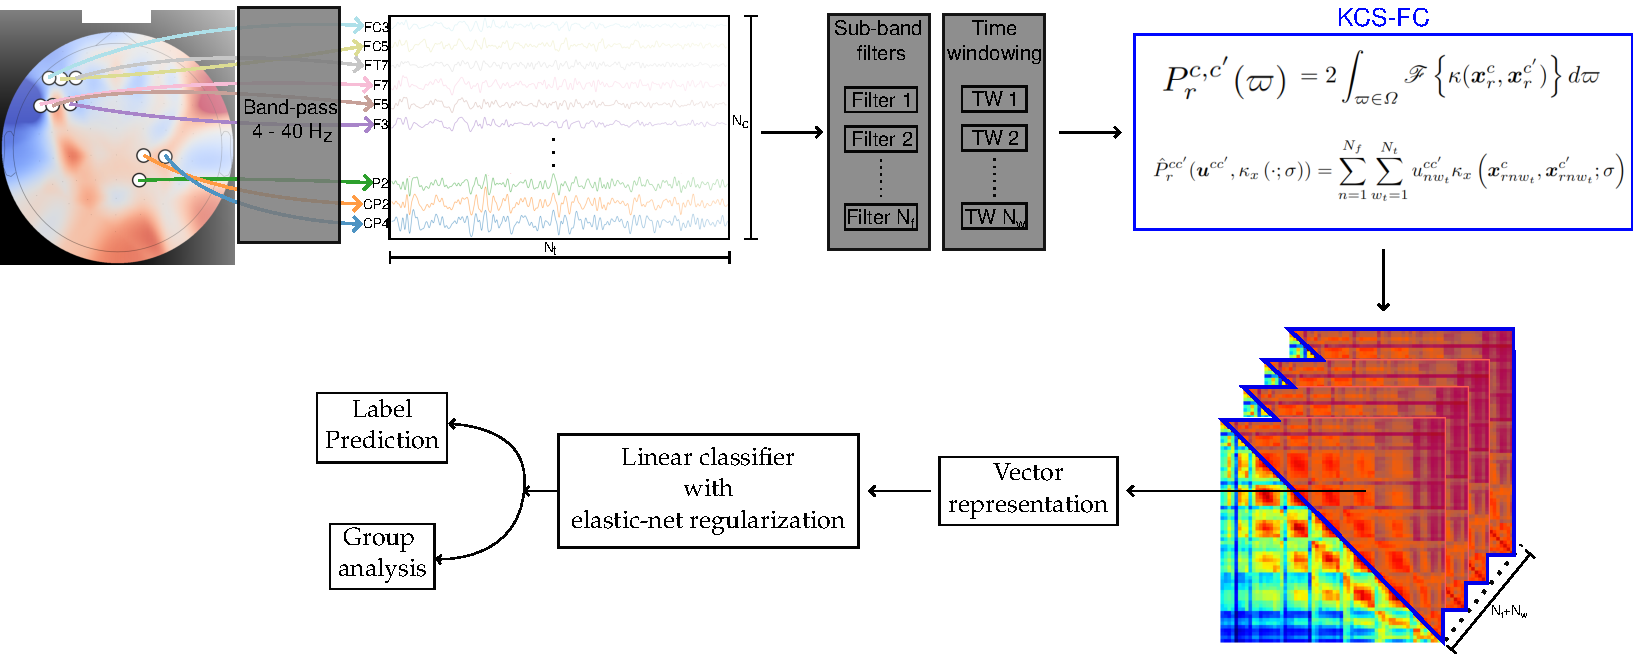
\includegraphics[scale=0.6]{Figures/outline_and_contributions/contribution1_C.pdf}
    \caption{Illustration of the proposed Kernel-based Cross-Spectral FC for enhancing the MI-BCI model's accuracy. Key features include robust FC estimators using a Gaussian kernel for non-linearity, short sliding windows for addressing non-stationarity, sub-band filtering for managing inter-subject variability, vectorization representation for FC extraction and elastic-net regularization to curb spurious connectivities \label{fig:contribution1}}
\end{figure}

\section{Kernel-based Covariance Function}
\changes{The Wiener-Khinchin's theorem states that a real-valued auto-correlation function, $R^{c}_{r}(\tau)$, of a weak-sense stationary stochastic process $x^{c}_{r}(\tau)$ can be defined as~\cite{cohen1998generalization}:
\begin{equation}\label{eq:wiener}
	R^{c}_{r}(\tau) = \int_{\varpi \in \Omega}\exp({j2\pi \tau \varpi})dP^{c}_{r}(\varpi) ,
\end{equation}
where $P^{c}_{r}(\varpi)\en\Real[0,1]$ is a monotonic spectral distribution function absolutely continuous and differentiable over frequency $\varpi \in \Omega$.
According to Bochner's theorem the univariable relationship in~Equation~\eqref{eq:wiener} a stationary positive-definite kernel \changes{$\kappa^{cc'}_{r}(\Delta_{x}) = \kappa(\ve{x}^{c}_{r},\ve{x}^{c'}_{r})$} can be related with its cross-spectral counterpart $S^{cc'}_{r}(\varpi)$ if and only if the following assumption holds between both spectral representations~\cite{bochner2020harmonic}:
\begin{equation}\label{eq:kCSD}
	\kappa^{cc'}_{r}(\Delta_{x}) = \int_{\varpi \in \Omega} \exp{(j2\pi {\Delta_{x}} \varpi)} S^{cc'}_{r}(\varpi)d\varpi,
\end{equation}
where $\Delta_{x} = \ve{x}^{c}_{r} - \ve{x}^{c'}_{r}$ is the vector delay, $\varpi\subseteq\varOmega$ is the frequency domain that contains the bandwidth set of analysis $\varOmega$, and $ S^{cc'}_{r}(\varpi)$ is the cross-spectral density that preserves the following equality: $ S^{cc'}_{r}(\varpi) = d {P}^{cc'}_{r}(\varpi)/d\varpi$, with $ P^{cc'}_{r}(\varpi)\en\Real[0,1]$ being the cross-spectral distribution that is related to the mapping kernel, $\kappa: \Real^{N_t} \times \Real^{N_t}\to \Real$.
As regards $\kappa(\ve{x}^{c}_{r},\ve{x}^{c'}_{r}) = \langle \phi(\ve{x}^{c}_{r}),\phi(\ve{x}^{c'}_{r}) \rangle_{\mathcal{H}}$, it is a positive-definite stationary kernel inducing the nonlinear feature mapping $\phi(\cdot)$ to a Reproducing Kernel Hilbert Space, $\mathcal{H}$. Notation $\langle \cdot,\cdot \rangle$ represents the dot product. 
Therefore, we compute the cross-spectral distribution $ P^{cc'}_{r}(\varpi)$ within a bandwidth $\varOmega$, as below:
\begin{equation}
	\begin{aligned}\label{eq:CSDist}
		P^{cc'}_{r}(\varpi) &= 2\int_{\varpi \in \varOmega} S^{cc'}_{r}(\varpi)d\varpi,\\
		&=2\int_{\varpi \in \varOmega} \mathscr{F}\left\{\kappa(\ve{x}^{c}_{r},\ve{x}^{c'}_{r}) \right\}d\varpi,
	\end{aligned}
\end{equation}
where notation $\mathscr{F}\{\cdot\}$ stands for the Fourier transform. 
}

As a result,~Equation~\eqref{eq:CSDist} preserves the frequency-based interpretation of the kernel-based pairwise dependencies that were estimated between vectors of random functions. Furthermore, the imposed stationary kernel favors the extraction of nonlinear data dependencies~\cite{bishop2006pattern}

\section{Gaussian Functional Connectivity from Kernel-based Spectral Distribution}
\changes{
Let $\ve{x}^{c}_{rnw_t}$ be an EEG channel $c$ at trial $r$ within filter $n$ and time window $w_t$, and $\{ \ve{x}^{c}_{rnw_t} \in \Real^{N_t}, {y}_r \in \Real[0,1]\}_{c,r,n,w_t=1}^{N_c,R,N_f,N_t}$ be an time segmented filtered EEG set holding all channels $N_c$, $R$ trials, $N_f$ frequency bandwidths, $N_t$ time windows , ${y}_r$ is the class or label assigned to the $r$-th trial, and the notation $|\cdot|$ stands for set cardinality. Since the Gaussian kernel is preferred in pattern classification because of its universal approximating ability and mathematical tractability~\cite{Alvarez-Meza2014}, we propose the Gaussian function to compute the pairwise kernel-based dependencies between channels $c$ and $c'$, without the case $c\neq c'$ in~Equation~\eqref{eq:kCSD}, termed Gaussian Functional Connectivity (KCS-FC), defined as follows:
\begin{equation}
		\kappa_x\left(\ve{x}^{c}_{rnw_t}, \ve{x}^{c'}_{rnw_t};\sigma\right) = \exp{\left( {-\|\ve{x}^{c}_{rnw_t}-\ve{x}^{c'}_{rnw_t}\|^2_2}/{2\sigma^2}\right)}, \label{eq:gkernel}
\end{equation}
where $\sigma\en\Real^+$ is the length scale hyperparameter. Notation $\|\cdot\|_q$ stands for $\ell_q$-norm.
}

With the aim to implement the single-trial extraction, \changes{we estimate the cross-spectral distribution $\hat{\mat{P}}^{cc'}_{r}$ between a pair of channels $c$ and $c'$ at trial $r$ as follows:}
\changes{
\begin{equation}\label{eq:fcc}
	\hat{P}^{cc'}_{r}(\ve{u}^{cc'},\kappa_x\left(\cdot;\sigma\right)) = \sum_{n=1}^{N_f}\sum_{w_t=1}^{N_t} u_{nw_t}^{cc'}\kappa_x\left(\ve{x}^{c}_{rnw_t},\ve{x}^{c'}_{rnw_t};\sigma\right),
\end{equation}
where $\ve{u}^{cc'} \in \Real^{N_f N_t}$ is the spatio-temporal-frequency (\textit{s-t-f}) relevance vector that codes the pairwise undirected dependency between channels and contains the values $u_{nw_t}^{cc'}$ holding the relevance value estimated at $n$-th frequency and $w_t$ window.
}

\changes{Using the single-trial kernel-based spectral distribution representation in~Equation~\eqref{eq:fcc}, we propose extracting the sparse functional connectivity, using the Elastic Net regularization \cite{tay2023elastic}, aiming to finding discriminative and interpretable brain activity patterns.
\begin{equation}\label{eq:SRC}
	\ve{u}^* = \arg \min_{\ve{u}} \promed{ \sum_{r=1}^{R} \left\|\sum_{c,c'=1}^{N_c}\hat{P}^{cc'}_{r}(\ve{u}^{cc'},\kappa_x(\cdot;\sigma))-y_r\right\|^2_2} + \alpha \sum_{c,c'=1}^{N_c}\|\ve{u}^{cc'}\|_1 + \frac{1-\alpha}{2} \sum_{c,c'=1}^{N_c}\|\ve{u}^{cc'}\|_2 \quad :  \forall c < c',
\end{equation}
where $\alpha \in \Real^+$ is the regularization hyperparameters, and $\| \cdot \|_q$ is the $\ell_q$-norm.
}

\changes{Without loss of generallity, equation~\eqref{eq:SRC} can be rewritten as:
\begin{equation}
	\ve{\tilde{u}}^* = \arg \min_{\ve{\tilde{u}}} \promed{\sum_{r=1}^{R} \|\ve{\tilde{u}}\ve{\tilde{p}_{r}}^{\top}-y_r\|^2_2} + \alpha \|\ve{\tilde{u}}\|_1 + \frac{1-\alpha}{2} \|\ve{\tilde{u}}\|_2, \label{eq:SRC_vec}
\end{equation}
where $\top$ is the vector transpose, $\ve{\tilde{u}}$ and $\ve{\tilde{\kappa}}$ stand for the spatio-temporal-frequency relevance matrix and cross-spectral distribution vector concatenation obtained as:
\begin{equation}
	\begin{aligned}
		\ve{\tilde{u}} &= \left[u_{11}^{12},u_{11}^{13},\cdots,u_{11}^{1N_c},u_{11}^{23},\cdots,u_{11}^{(N_c-1)N_c},u_{12}^{12},\cdots, u_{N_fN_t}^{(N_c-1)N_c} \right], \\
		\ve{\tilde{p}}_{r} &= \left[ \hat{P}_{r11}^{12},\hat{P}_{r11}^{13},\cdots,\hat{P}_{r11}^{1N_c},\hat{P}_{r11}^{23},\cdots,\hat{P}_{r11}^{(N_c-1)N_c},\hat{P}_{r12}^{12},\cdots, \hat{P}_{rN_fN_t}^{(N_c-1)N_c} \right] ,\\
	\end{aligned}
\end{equation}
Note that for simplicity the term $\hat{P}^{cc'}_{r}(\mat{U}^{cc'}_{r},\kappa_x\left(\cdot;\sigma\right))$ is rewritten as $\hat{P}^{cc'}_{rnw_t}$.
}

Consequently, the optimization framework in~Equation~\eqref{eq:SRC_vec} allows for computing the spectral combination weights from the extracted filter-bank representations that match the MI class-probability set, resulting in a sparse, relevant kernel-based functional connectivity between pairs of EEG channels.


\section{Experimental Set-Up}
The evaluation of the considered functional connectivity measures for enhanced feature extraction is performed according to the following stages: 

\changes{
({i}) Preprocessing and trial-based extraction of {s-t-f} representations. For extracting the subject EEG dynamics over time accurately, the sliding window length of feature extraction is fixed to the next values: $\tau=[0.5,1.0,1.5,2.0]$\,{s}, having an overlap of $75\%$. Additionally, similar to authors in \cite{ang2008filter} the frequency bands of interest are selected with the lower frequency limit set at 4 Hz, the upper limit set to 40 Hz, and an overlap of $50\%$.
}

\changes{
({ii}) The estimation of the single-trial functional connectivity from the extracted {s-t-f} features. For comparison, the proposed KCS-FC is contrasted with two commonly used single-trial FC measures. To facilitate this comparison, the KCS-FC in Equation~\eqref{eq:SRC} is interchanged with new single-trial FC measures. These measures can be estimated from a frequency $n$, a time window $w_t$, and a pair of channels ${cc'}$ (with $c \neq c'$, for all $cc'$ in $C$) as described in~\cite{rodrigue2019}.
\begin{equation}
			\rho(\ve{x}^{c}_{rnw_t},\ve{x}^{c'}_{rnw_t}) ={\left<\ve{x}^{c}_{rnw_t},\ve{x}^{c'}_{rnw_t}\right>}\label{Eq:Pearson}
\end{equation}
\begin{equation}		 
	{\Delta\phi(\ve{x}^{c}_{rnw_t},\ve{x}^{c}_{rnw_t})}  {= {|\exp(j(\ve{\phi}_{rnw_t}^{c}-\ve{\phi}_{rnw_t}^{c}))|}} \label{Eq:PLV} 
\end{equation}
}
where $\ve{x}^{c}_{rnw_t}$ and $\ve{x}^{c'}_{rnw_t}$ is the real-valued EEG data from the corresponding electrodes at trial $r$ (within temporal window $w_t$ and frequency band $n$) with instantaneous phases $\ve{\phi}_n^{ct}$ and $\ve{\phi}_n^{c't}$, respectively. The pairwise relationships in~Equations~\eqref{Eq:Pearson} and~\eqref{Eq:PLV} are referred as {Cross-Correlation Coefficient}(CCF) and {Phase Lag Value} (PLV), respectively.

{For feeding the classifier procedure, we evaluate two feature representation approaches that are extracted from each tested FC measure: Firstly, the feature representation is the CSP's pattern vector (linear projection of the sample covariance), computed as detailed in~\cite{velasquez2020dynamic}; in particular, the well-known CSP's eigendecomposition is applied by replacing the covariance matrix with the corresponding FC measure. Secondly,  the concatenated (vectorized) triangular representation of the symmetrical FC matrices is extracted, as detailed in~\cite{barachant2013classification}. Both of the approaches comprise a filter-bank-based concatenation strategy through a fixed sliding window size and overlap values; that is, the temporal dependencies between windows are not directly modeled.}

({iii}) Sparse feature selection and classifier performance computation. {Here, for implementation purposes, the optimizing problem is solved through the well-known Elastic-net algorithm to deal appropriately with redundant information. It is worth noting that we prefer Elastic-net over the Lasso-based regularization, because, when the number of features is greater than the number of training samples, Lasso behaves erratically~\cite{geron2022hands}.}

For comparative purposes, we also perform feature extraction using the baseline CSP-based spatial filtering that is widely used for filtering measures of synchronization~\cite{haddad2019early,kumar2018eeg}. To this end, we perform the CSP feature extraction, adjusting the sliding time window length at each evaluated value of $\tau$ and fixing the variance of the surrogate space to the first three eigenvectors of the spatial filtering matrix, as suggested in~\cite{lotte2018review}. It is worth mentioning that we evaluate the FC measures in~Equations~\eqref{Eq:Pearson} and \eqref{Eq:PLV}, as well the CSP-based feature extraction scheme, through the sparse model presented in~Equation~\eqref{eq:SRC} using a vector concatenation approach through temporal windows and frequency bands.

({iv}) Clustering of subject inefficiency and interpretation analysis. 
For enhancing the interpretive analysis, we cluster the differences in neural responses that depend on the users' motor skills. The intra/inter-subject variability affects the FC estimators' robustness properties, becoming stronger for the worst-performing individuals.

{Regarding the performance measure, the classifier accuracy $a_c\en[0,1]$ is computed, as follows:
$$a_c= \,(T_P \s{~+~} T_N )/ (T_P\s{~+~} T_N \s{~+~} F_P \s{~+~} F_N ),$$
 where $T_P$, $T_N$, $F_P$, and $F_N$ are true-positives, true-negatives, false-positives, and false-negatives, respectively. A stratified $10$-fold cross-validation strategy randomly partitions the training and testing sets.}

\section{Results and Discussion}

\subsection{Influencing FC Parameters on Accuracy Estimation}

\subsubsection{Impact of Prior CSP Filtering}

{\changes{For} interpretation purposes, Figure \ref{Fig:FCx} presents the subjects' accuracy in decreasing order by all evaluated EEG data collections. Each data set is tested in two configurations to feed the sparse feature selector: using feature concatenation (odd rows) and linearly mapping through CSP (even rows). The FC measures' accuracy is estimated at each $\tau$ ({PLV}---left column, {CCF}---middle column, {KCS-FC}---right column), adjusting the parameter $\sigma$ to the median averaged over the input distances for kernel-based functional connectivity computation.} 

{The top plots display the results that were performed by the databases with a similar amount of subjects: DMBI MI (first and second rows) and DB DBII ME (third and fourth rows). As seen, PLV yields the most scattered outcomes, with a significant portion accomplishing low accuracy.} {A similar situation holds for DBIII MI with a more visible subject variability: PLV discriminates the worst, followed by CCF, and KCS-FC performs a bit better, still outperforming the other FC when compared and having the accuracy values less spread throughout the subject set}. However, the accuracy estimates are significantly more dispersed across the individuals than in DBII ME, regardless of the FC measure. Several factors may account for the higher variability of MI data. The EEG montage of MI protocols is more complex ($64$ MI channels vs. $44$ ME channels). Besides, the ME signals are reported as having a higher degree of regularity than MI practicing, at least in terms of motor-related discriminability~\cite{shamsi2020early}. Consequently, even if the DBIII MI collection doubles the number of trials compared with DBII ME, the subject variability of MI data remains high enough to limit the CSP effectiveness (see the bottom row). Moreover, numerous subjects achieve accuracy values that are below $60\%$, which is, under the BCI-inefficiency level reported~\cite{Sanelli2019}. 

\subsubsection{Influence of Sliding Windows}

\Cref{Fig:AccTau} summarizes \changes{impact of the sliding window's length} on the classifier discrimination ability using each evaluated measure of FC. In the case of DBI MI, the first row shows that PLV and CCF both obtain very close performance if the CSP filtering is not involved at all tested window values. Otherwise, the latter measure notably improves in performance. Nevertheless, the proposed KCS-FC outperforms, and this behavior remains valid in the second row that presents the accuracy of DBII ME with more subject variability, as shown by the average bars. However, some fluctuations in the PLV and CCF performance are more evident after applying CSP, depending on the window. Instead, the KCS-FC measure presents performance nearly invariant across the range of considered sliding window lengths, being slightly enhanced by the CSP filtering algorithm.

\changes{Additionally}, the bottom row presents the classifier performance that is obtained by MI activity (DBIII MI) with the most challenging subject variability, showing that the accuracy of all FC measures drops, particularly in the case of PLV. As seen, the PLV and CCF accuracy values are more sensitive to the sliding window influence, while the proposed KCS-FC assessments remain constant over the range of $\tau$. One more aspect to highlight is that the CSP-based filtering effectiveness becomes more dependent on the specific sliding window selected. Furthermore, under increased subject variability, this spatial filtering method's application noticeably decreases the KCS-FC performance.

\subsection{Estimated Classifier Accuracy of Individuals}

The following consideration is linked to the quality of individual FC assessments because of their diverse variability. For this purpose, Figure \ref{Fig:IndividualAcc} illustrates the individual classifier performance at each window length, for which the subjects are displayed on the horizontal axis in decreasing order of the CCF accuracy achieved at $\tau=2$\,{s} (the continuous line outlined in blue color). The rationale for choosing this specific FC estimation case as the baseline is that the cross-correlation coefficient that is presented in~Equation~\eqref{Eq:Pearson} can be directly associated with the conventional Pearson estimate with the simplest interpretation regarding pairwise relationships~\cite{georgiadis2019connectivity}.

\def \kerrwidth {.2\linewidth}
\begin{figure}[h!]
\centering
	\hbox{\hspace{4.5cm} {PLV}\hspace{2.6cm} {CCF}\hspace{2.7cm} {KCS-FC}}
	\rotatebox{90}{ \quad\, \textbf{\tiny DBI MI}}
	\rotatebox{90}{\quad\,\tiny{Accuracy ($\%$)}}
	{\resizebox{\kerrwidth}{!}{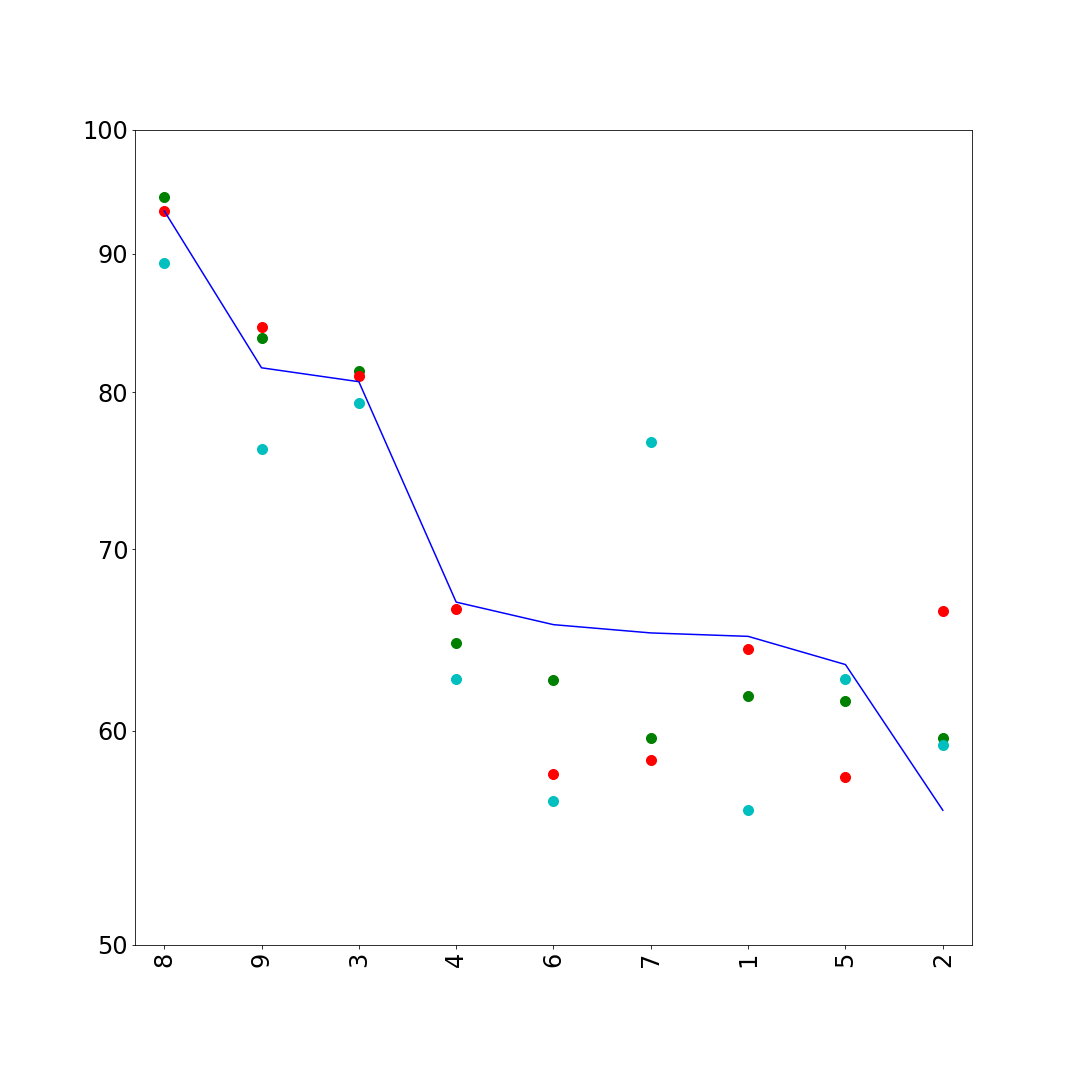
\includegraphics[trim=85 100 80 80, clip]{Figures/Objective_1/taus_plv_BCI_MI.png}}}
	{\resizebox{\kerrwidth}{!}{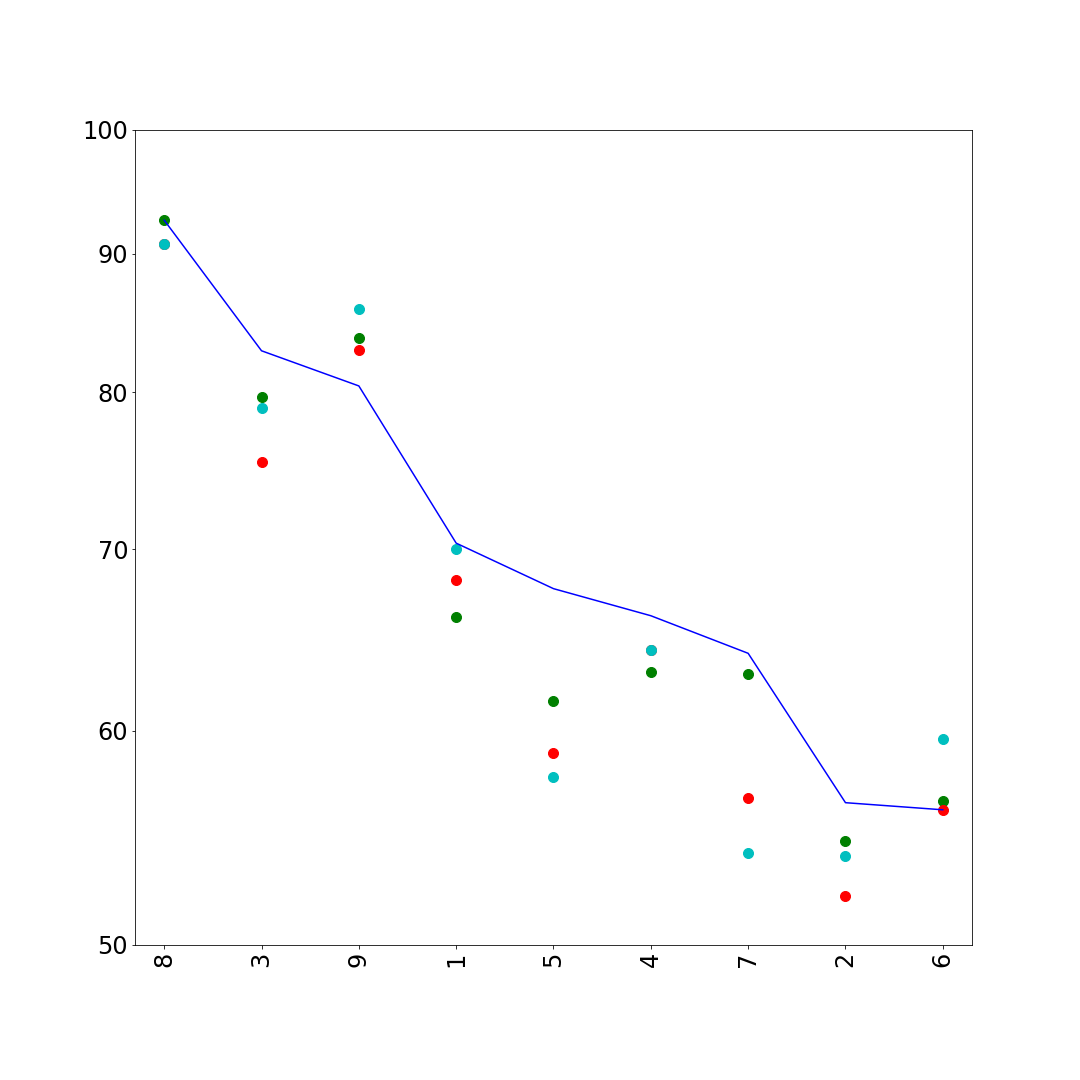
\includegraphics[trim=85 100 80 80, clip]{Figures/Objective_1/taus_pearson_BCI_MI.png}}}
	{\resizebox{\kerrwidth}{!}{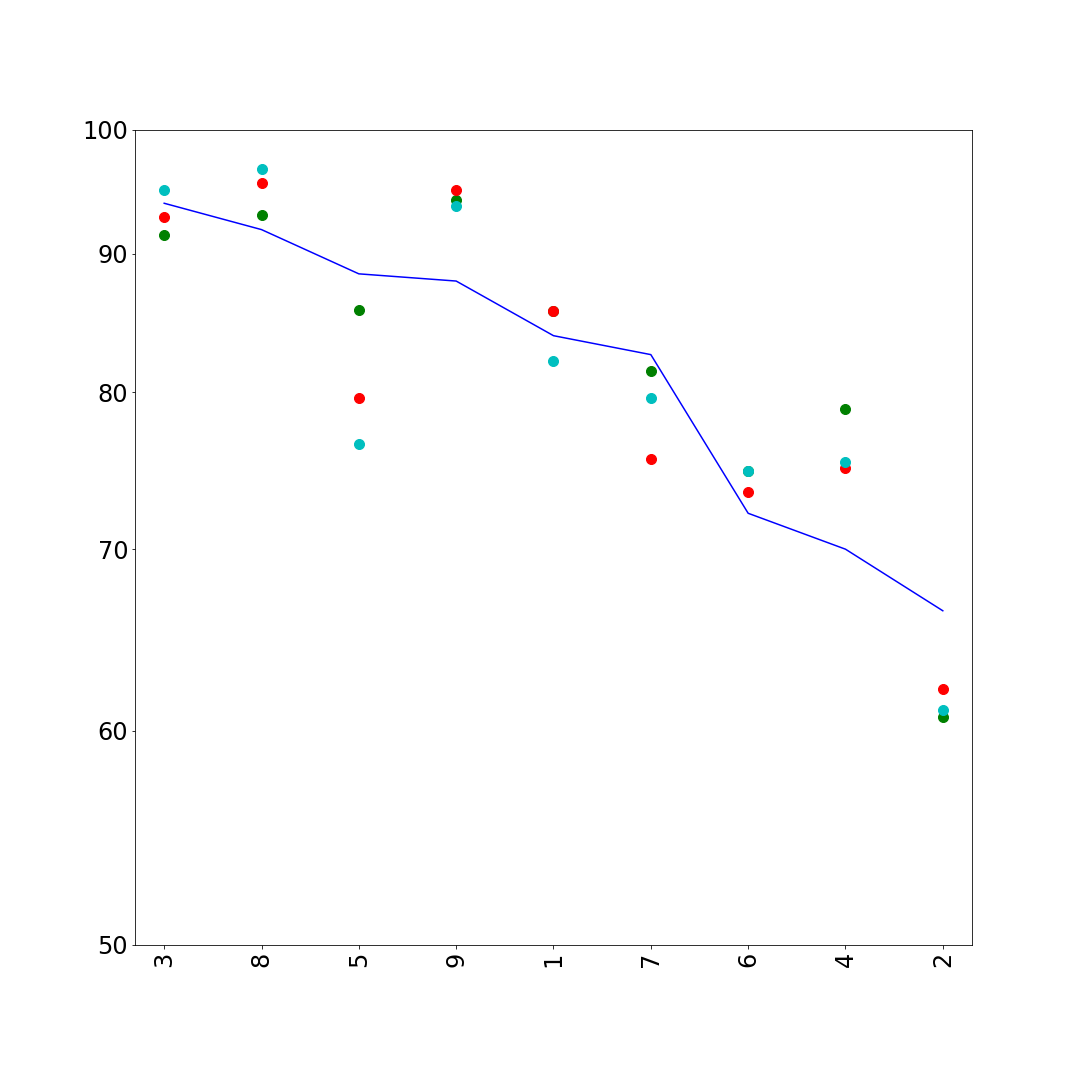
\includegraphics[trim=85 100 80 80, clip]{Figures/Objective_1/taus_gauss_BCI_MI.png}}}\\	
	\rotatebox{90}{ \quad\, \textbf{\tiny DBI MI-CSP} }
	\rotatebox{90}{\quad\,\tiny{Accuracy ($\%$)}}
	{\resizebox{\kerrwidth}{!}{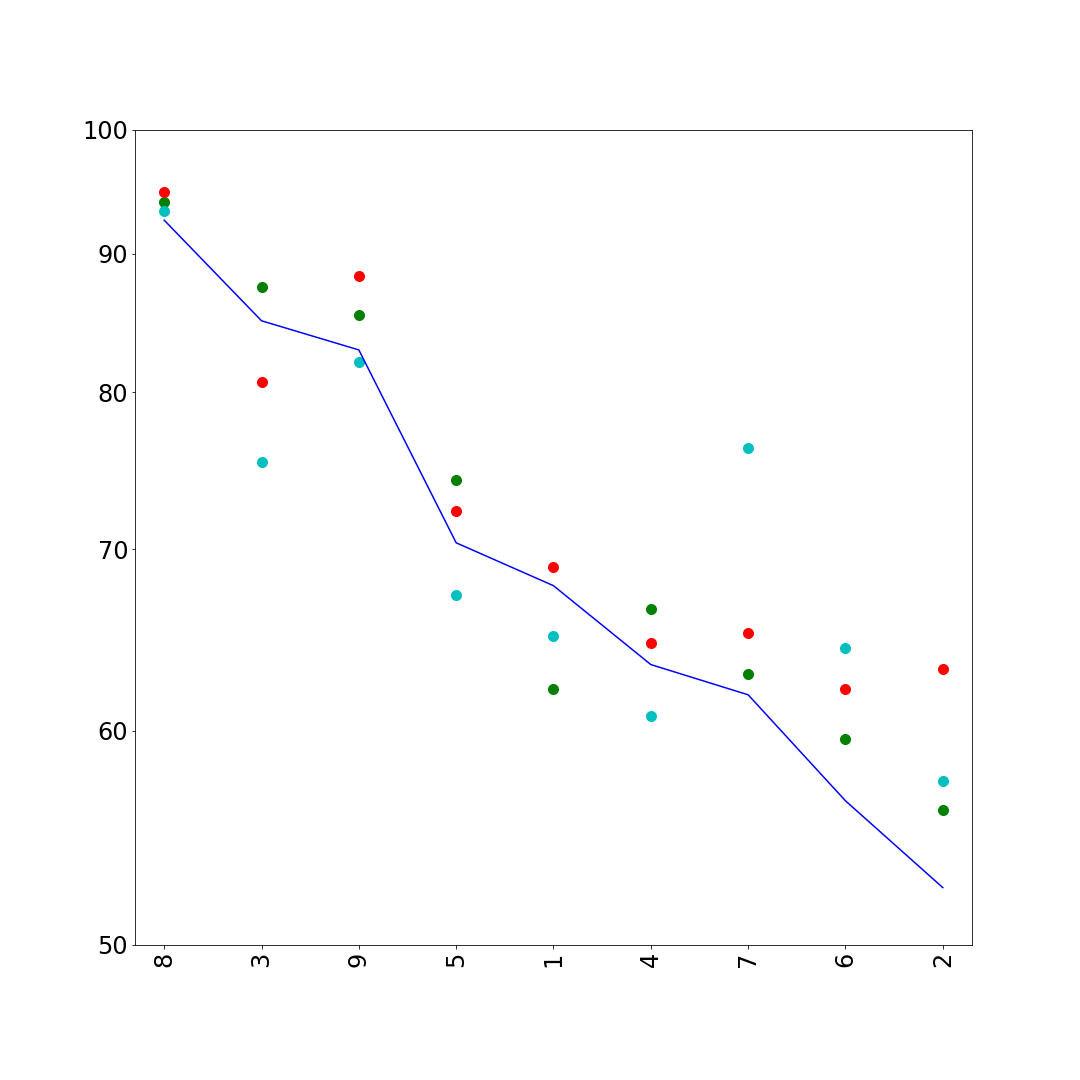
\includegraphics[trim=85 100 80 80, clip]{Figures/Objective_1/taus_csp_plv_BCI_MI.png}}}
	{\resizebox{\kerrwidth}{!}{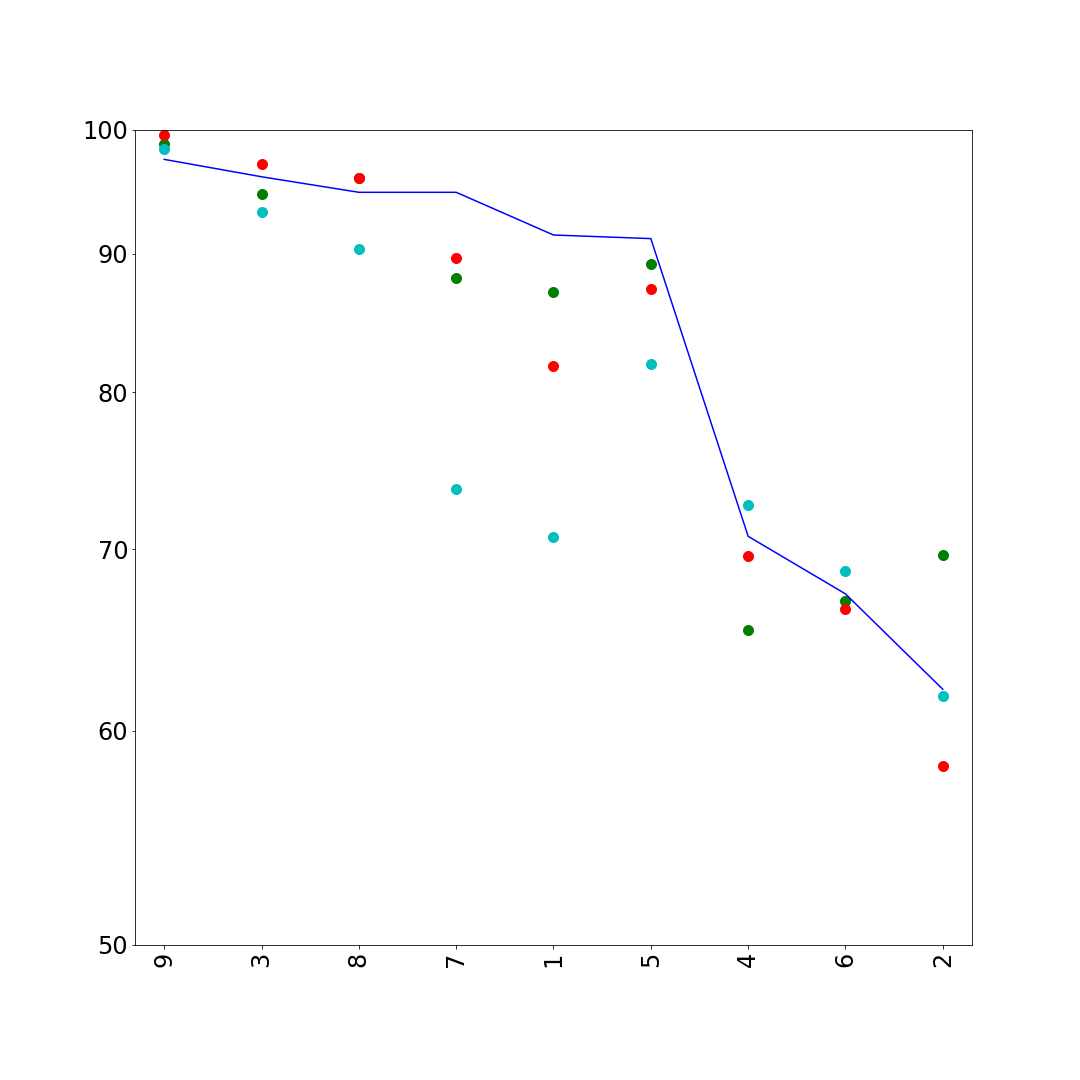
\includegraphics[trim=85 100 80 80, clip]{Figures/Objective_1/taus_csp_pearson_BCI_MI.png}}}
	{\resizebox{\kerrwidth}{!}{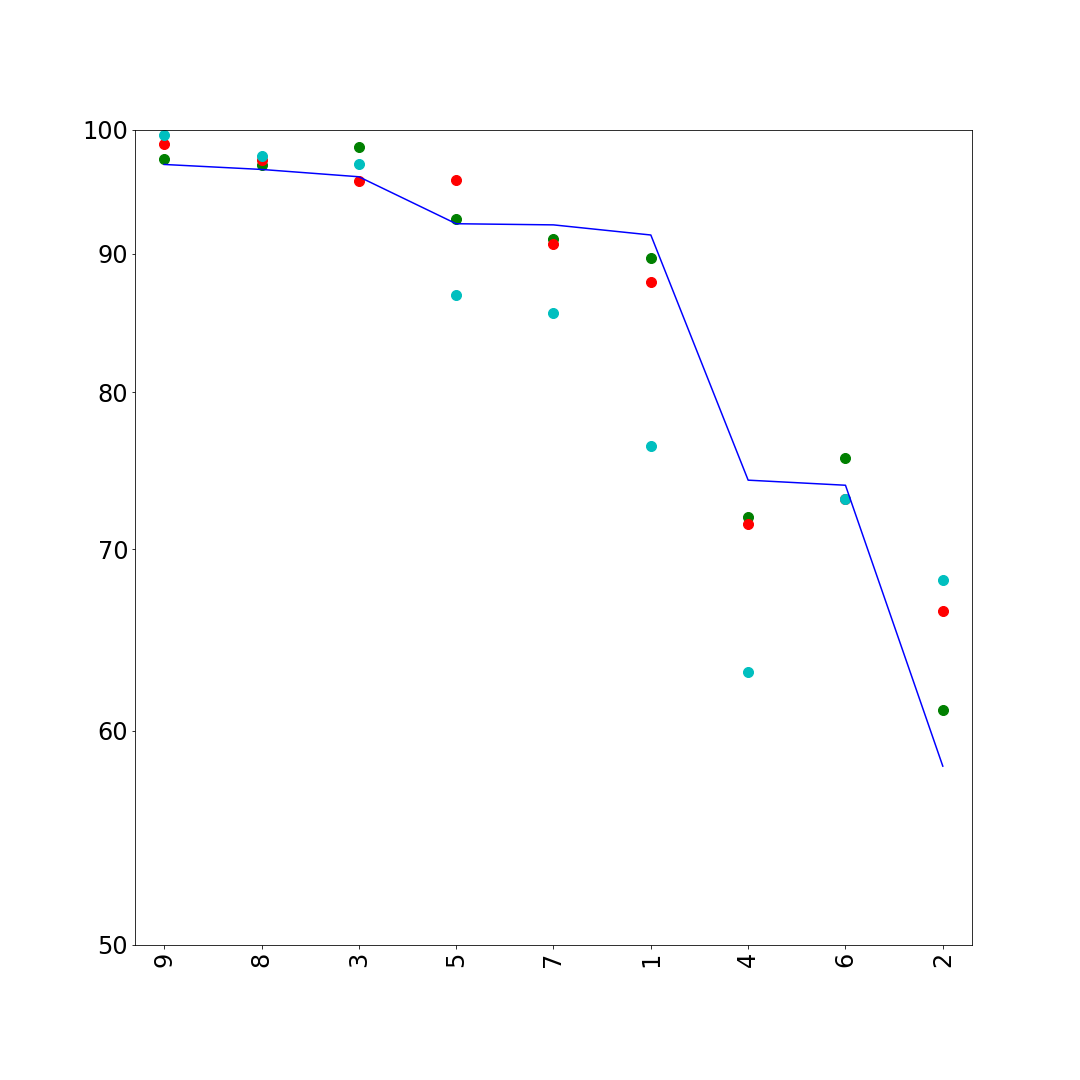
\includegraphics[trim=85 100 80 80, clip]{Figures/Objective_1/taus_csp_gauss_BCI_MI.png}}}\\	
	\rotatebox{90}{ \quad\, \textbf{\tiny DBII ME}}
	\rotatebox{90}{\quad\,\tiny{Accuracy ($\%$)}}
	{\resizebox{\kerrwidth}{!}{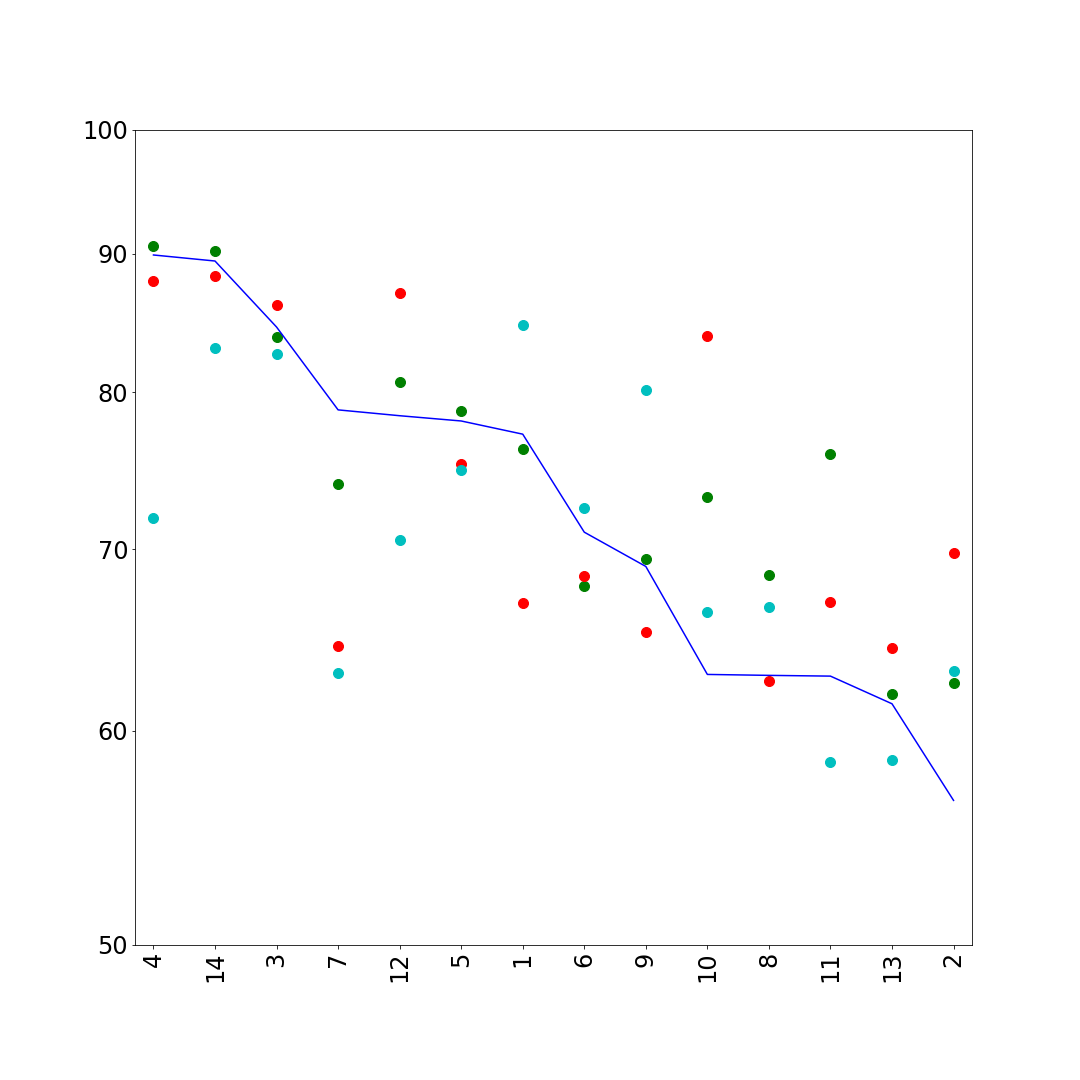
\includegraphics[trim=85 100 80 80, clip]{Figures/Objective_1/taus_plv_HG_ME.png}}}
	{\resizebox{\kerrwidth}{!}{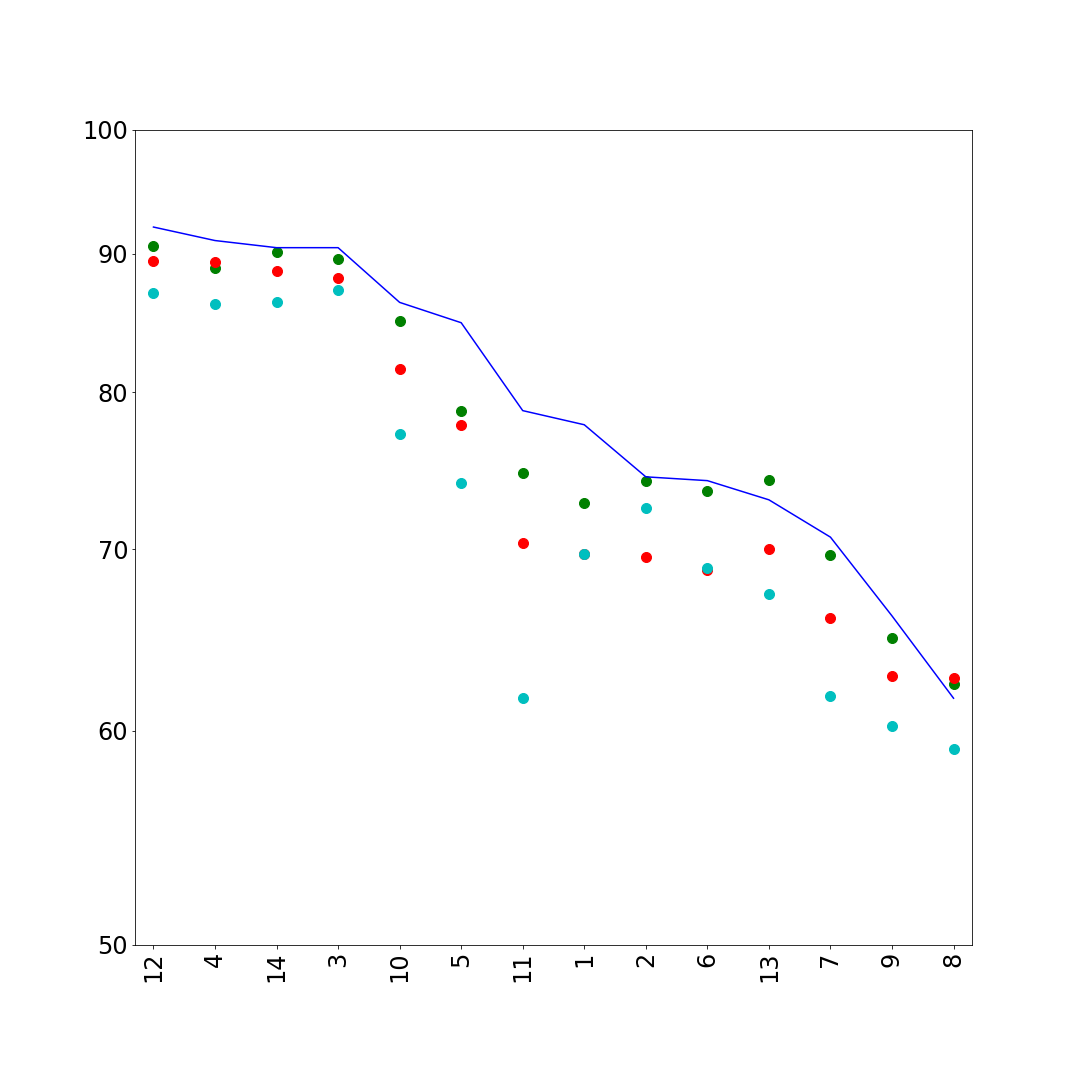
\includegraphics[trim=85 100 80 80, clip]{Figures/Objective_1/taus_pearson_HG_ME.png}}}
	{\resizebox{\kerrwidth}{!}{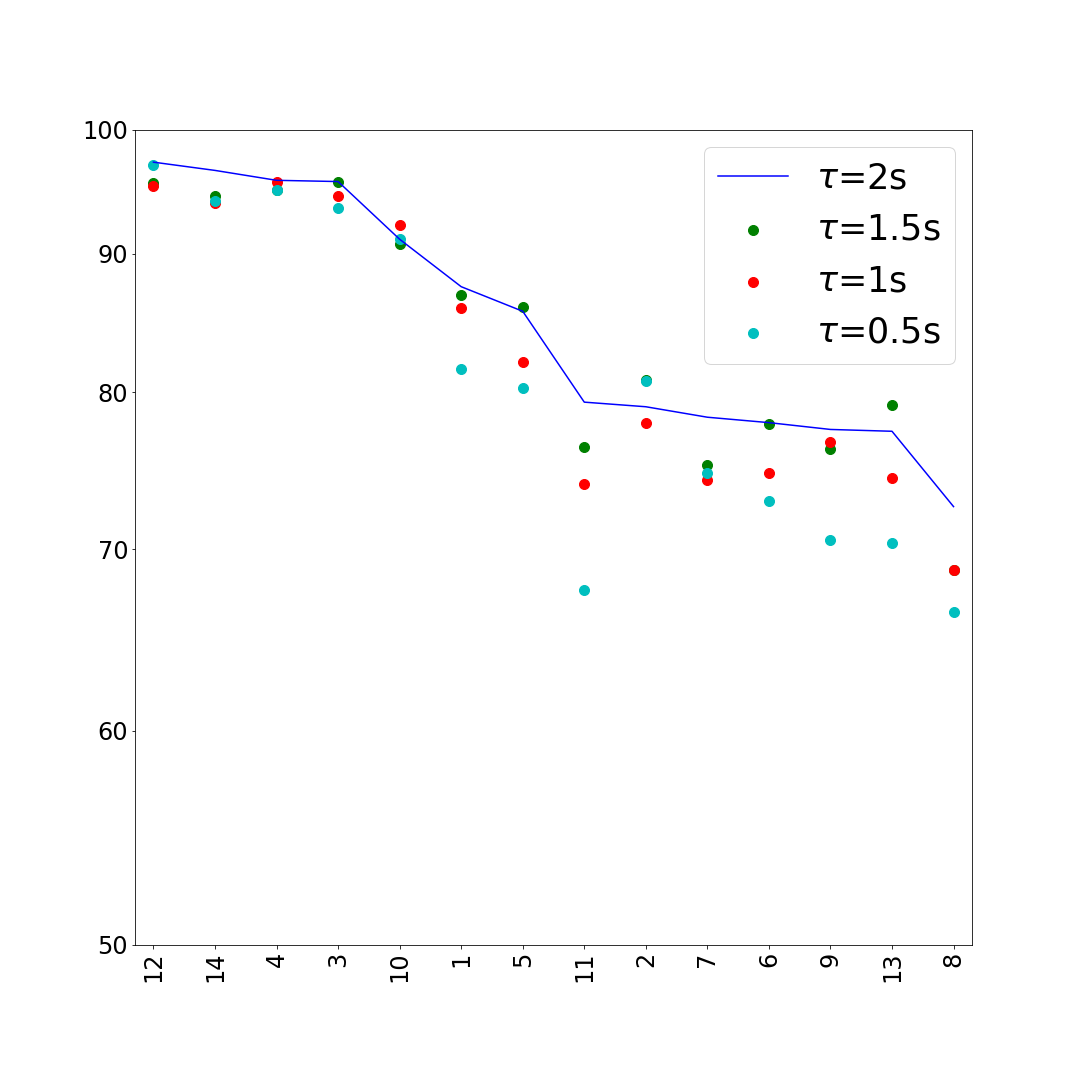
\includegraphics[trim=85 100 80 80, clip]{Figures/Objective_1/taus_gauss_HG_ME.png}}}\\
	\rotatebox{90}{ \quad\, \textbf{\tiny DBII ME-CSP}}
	\rotatebox{90}{ \quad\,\tiny{Accuracy ($\%$)}}
	{\resizebox{\kerrwidth}{!}{\includegraphics[trim=85 100 80 80, clip]{Figures/Objective_1/taus_CSP_plv_HG_ME.png}}}
	{\resizebox{\kerrwidth}{!}{\includegraphics[trim=85 100 80 80, clip]{Figures/Objective_1/taus_CSP_pearson_HG_ME.png}}}
	{\resizebox{\kerrwidth}{!}{\includegraphics[trim=85 100 80 80, clip]{Figures/Objective_1/taus_CSP_gauss_HG_ME.png}}}\\
	\rotatebox{90}{ \quad\, \textbf{\tiny DBIII MI}}
	\rotatebox{90}{ \quad\,\tiny{Accuracy ($\%$)}}
	{\resizebox{\kerrwidth}{!}{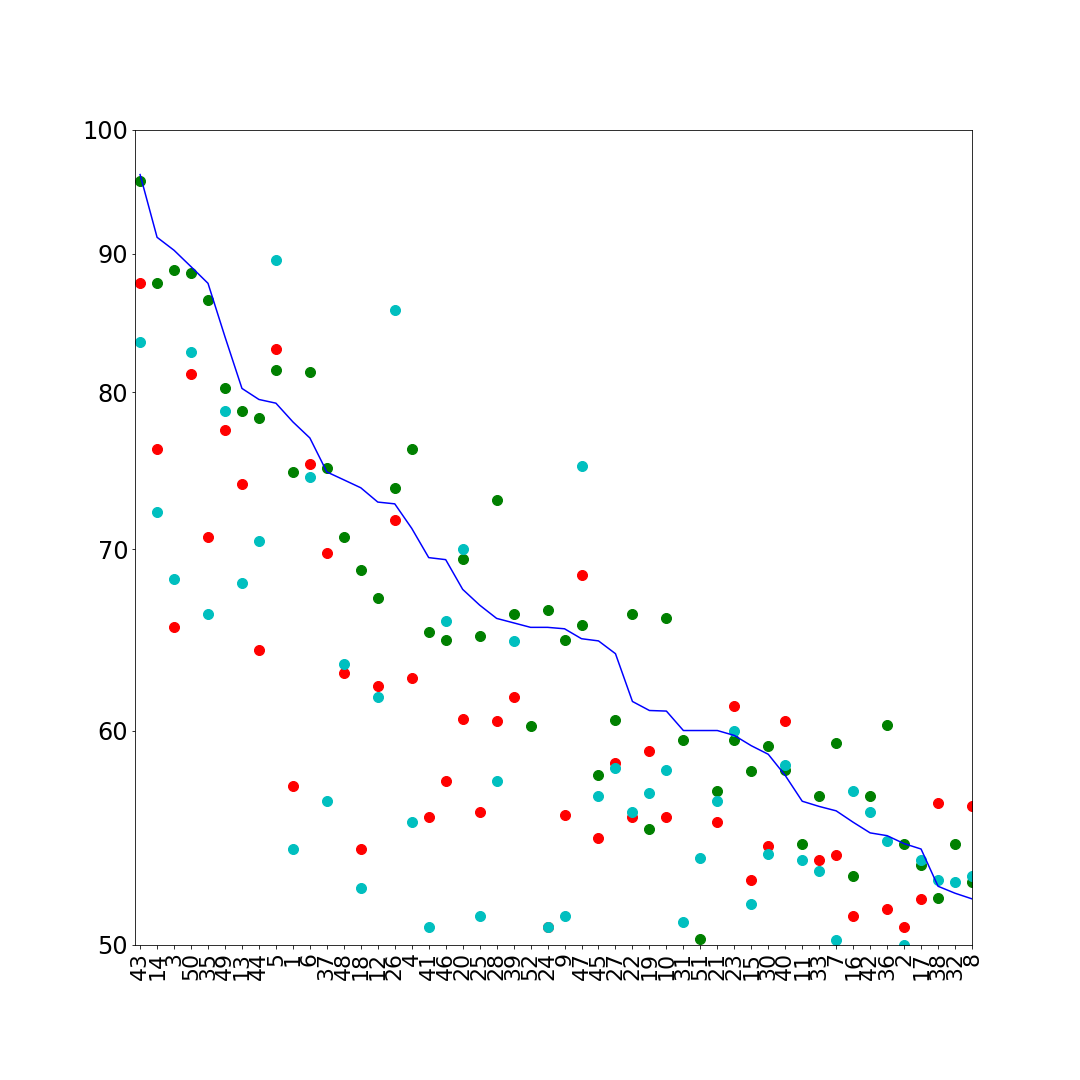
\includegraphics[trim=85 100 80 80, clip]{Figures/Objective_1/taus_plv_giga_MI.png}}}
	{\resizebox{\kerrwidth}{!}{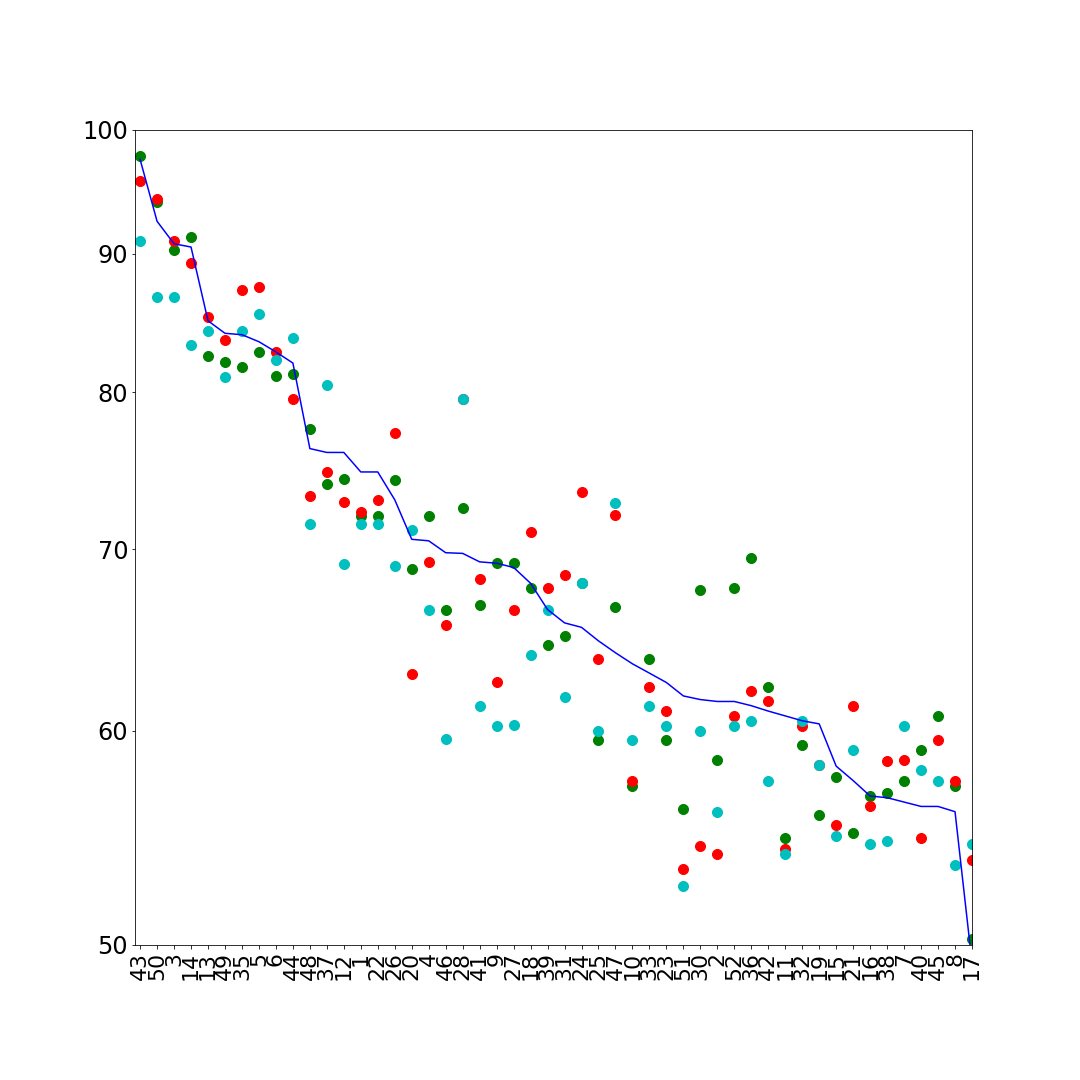
\includegraphics[trim=85 100 80 80, clip]{Figures/Objective_1/taus_pearson_giga_MI.png}}}
	{\resizebox{\kerrwidth}{!}{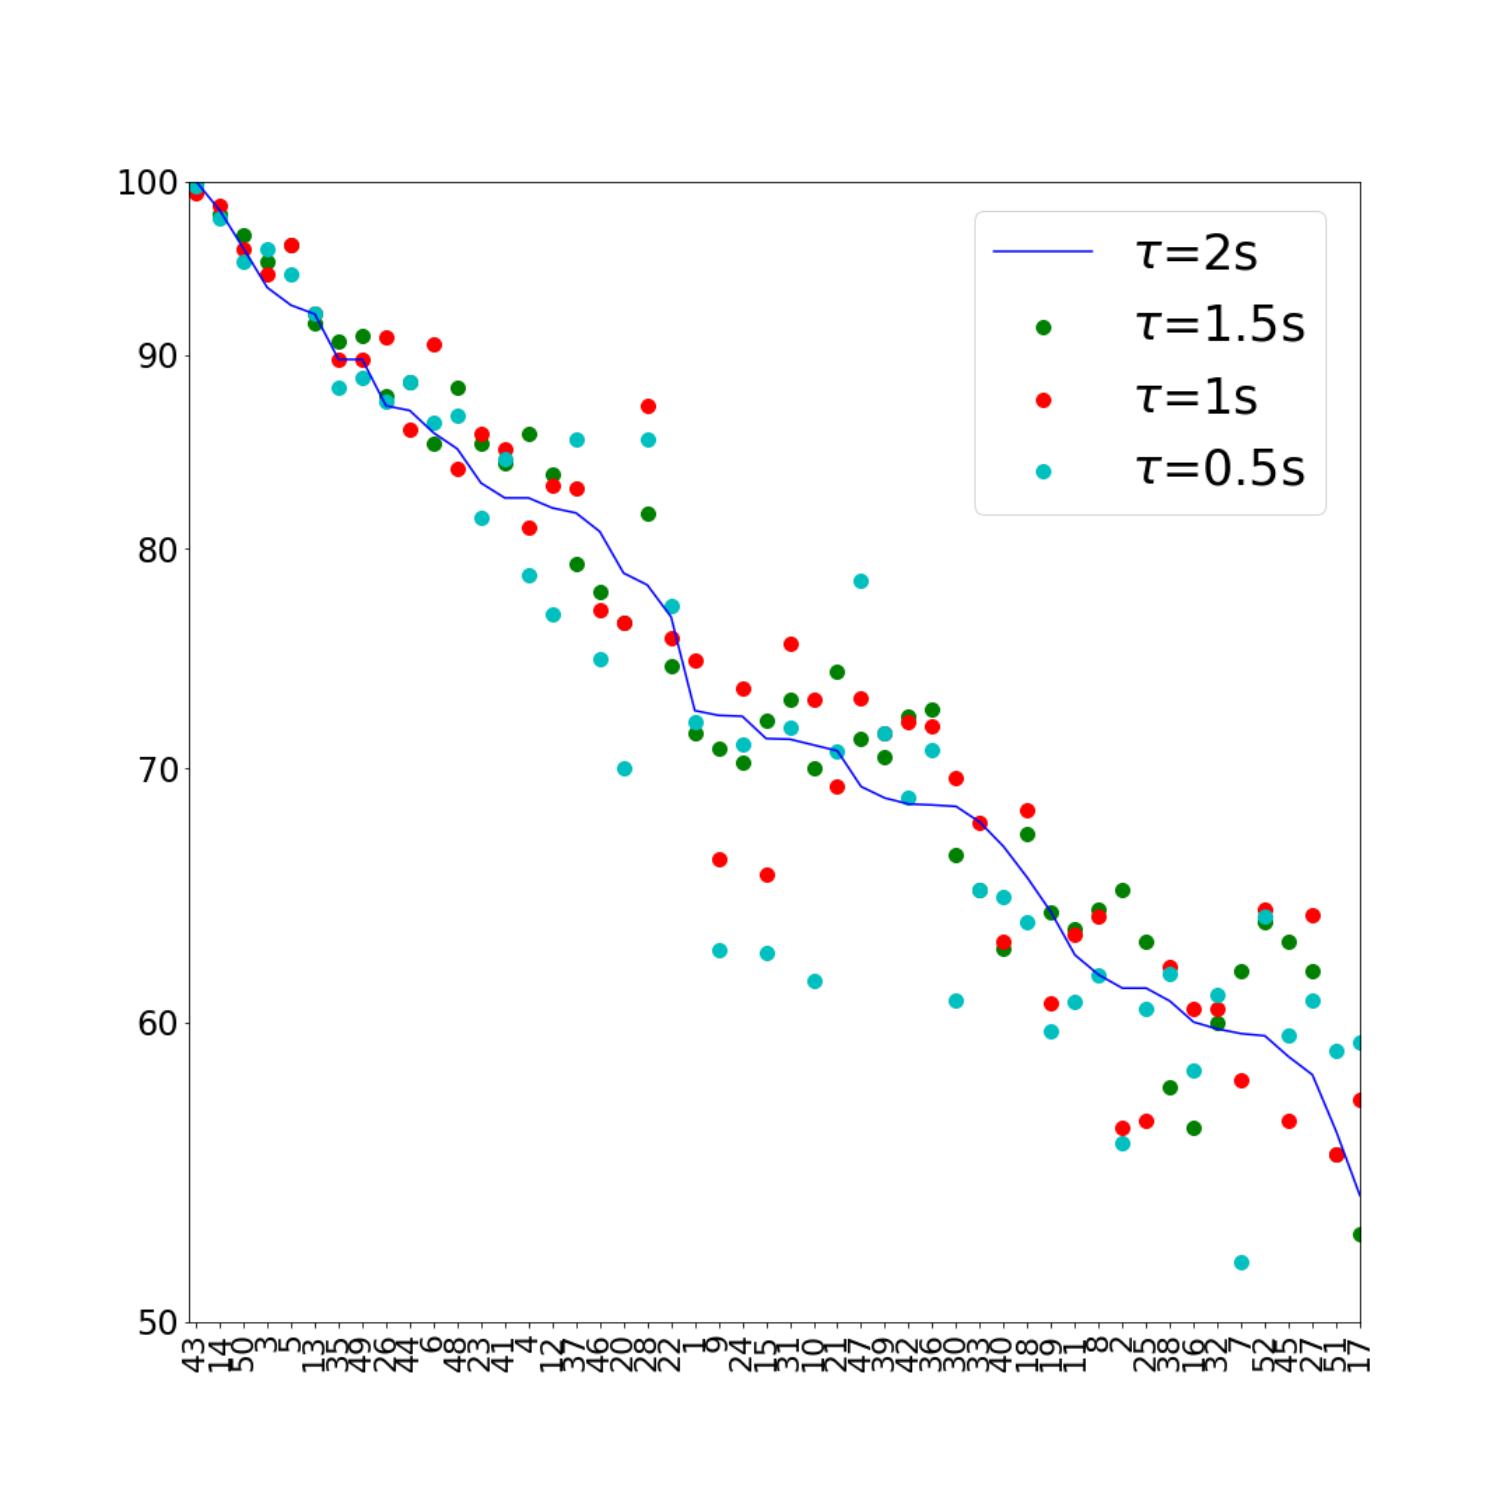
\includegraphics[trim=85 100 80 80, clip]{Figures/Objective_1/taus_gauss_giga_MI.png}}}\\
	\rotatebox{90}{\quad \textbf{\tiny DBIII MI-CSP}}
	\rotatebox{90}{ \quad\,\tiny{Accuracy ($\%$)}}
	{\resizebox{\kerrwidth}{!}{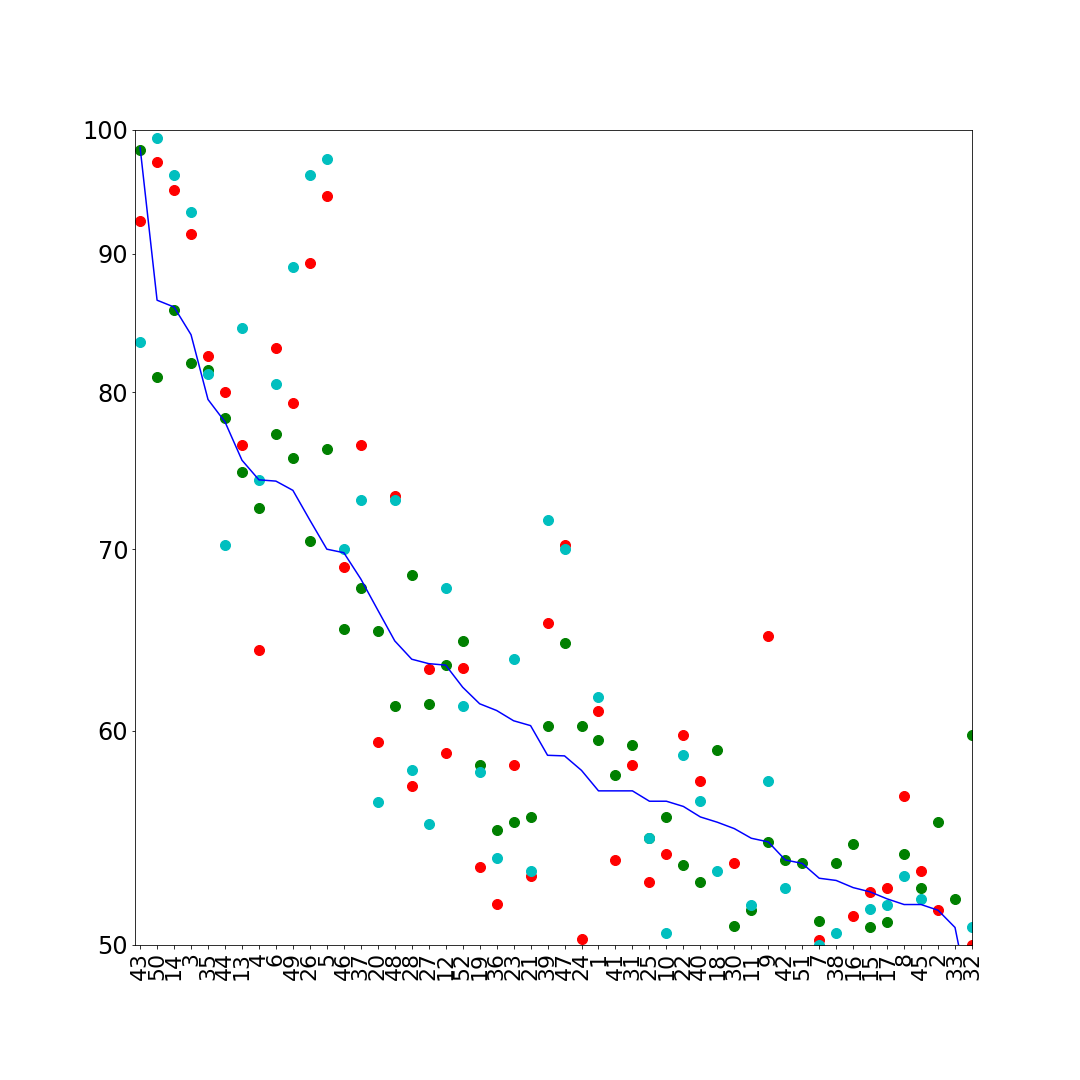
\includegraphics[trim=85 100 80 80, clip]{Figures/Objective_1/taus_csp_plv_giga_MI.png}}}
	{\resizebox{\kerrwidth}{!}{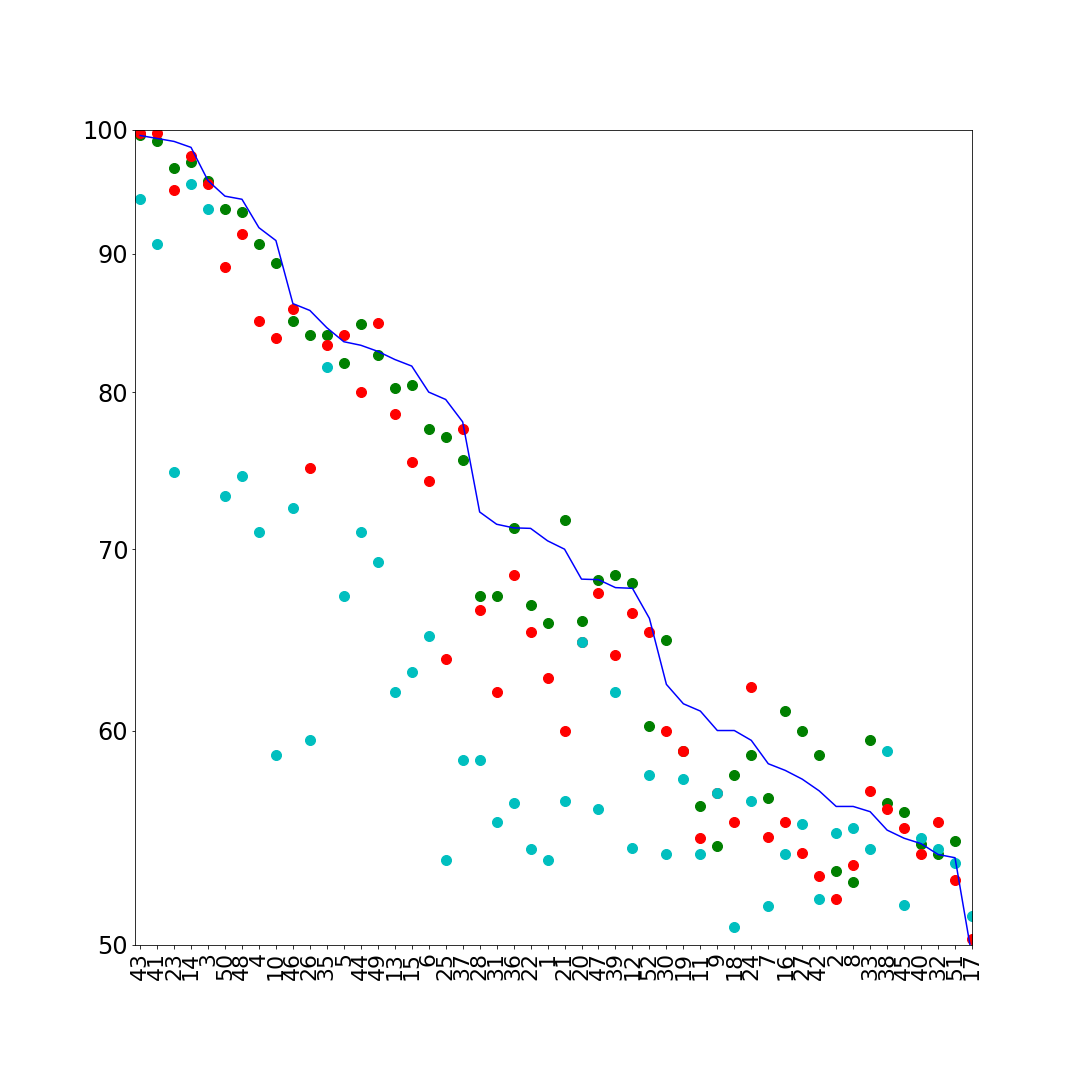
\includegraphics[trim=85 100 80 80, clip]{Figures/Objective_1/taus_csp_pearson_giga_MI.png}}}
	{\resizebox{\kerrwidth}{!}{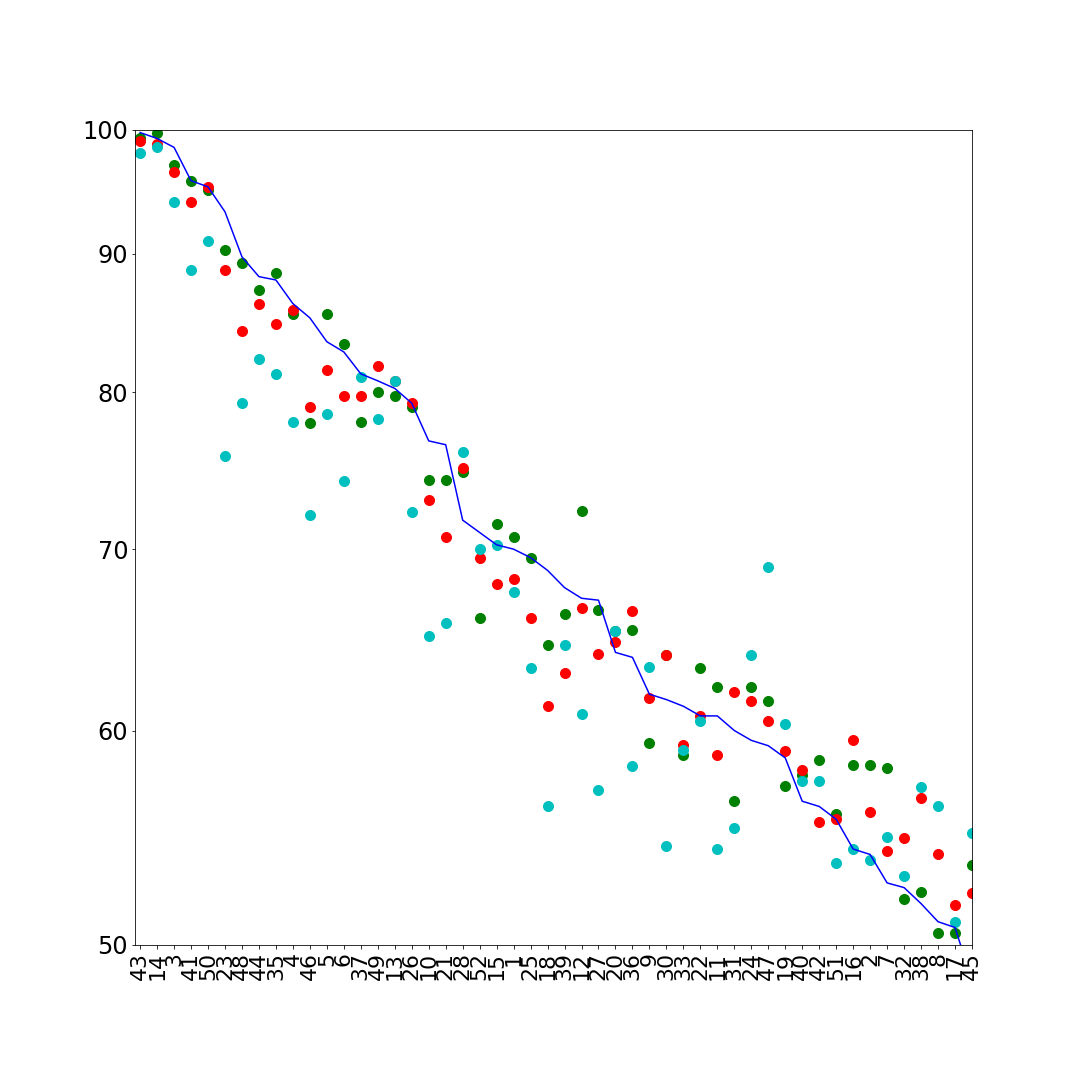
\includegraphics[trim=85 100 80 80, clip]{Figures/Objective_1/taus_csp_gauss_giga_MI.png}}}\\
	\hbox{\hspace{1.9cm} \tiny{Subject id}\hspace{2.8cm} \tiny{Subject id}\hspace{2.9cm} \tiny{Subject id}}
	\caption{{Subject accuracy at each window length $\tau$ performed by the evaluated FC measures: PLV,~CCF, and KCS-FC. Subjects are displayed on the horizontal axis in decreasing order of each FC accuracy at $\tau=2$\,{s}. Notation CSP stands for the accuracy estimated after the spatial CSP filtering.} }\label{Fig:FCx}
\end{figure}

\def \kerrwidth {0.93\linewidth} 
\begin{figure}[h!]
\centering
	\rotatebox{90}{\qquad \quad\, \textbf{DBI-MI}}
	\rotatebox{90}{\qquad \quad\, \footnotesize{Accuracy ($\%$)}}
	{\resizebox{\kerrwidth}{!}{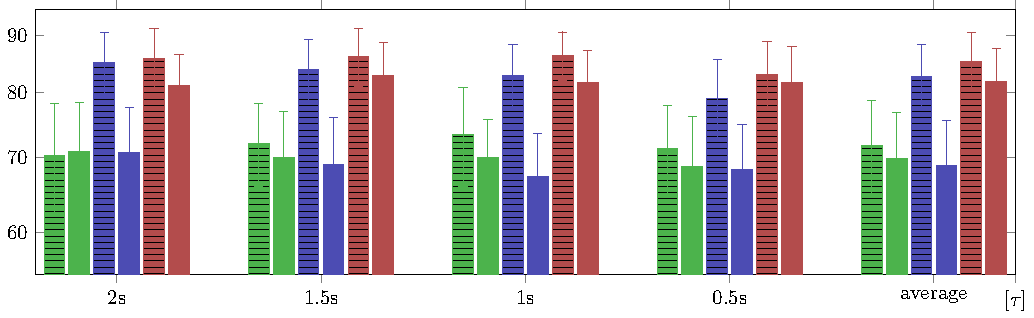
\includegraphics{Figures/Objective_1/acc_regularizacionDBII}}}\\
	\rotatebox{90}{\qquad \quad\, \textbf{DBII-ME}}
	\rotatebox{90}{\qquad \quad\,\footnotesize{Accuracy ($\%$)}}
	{\resizebox{\kerrwidth}{!}{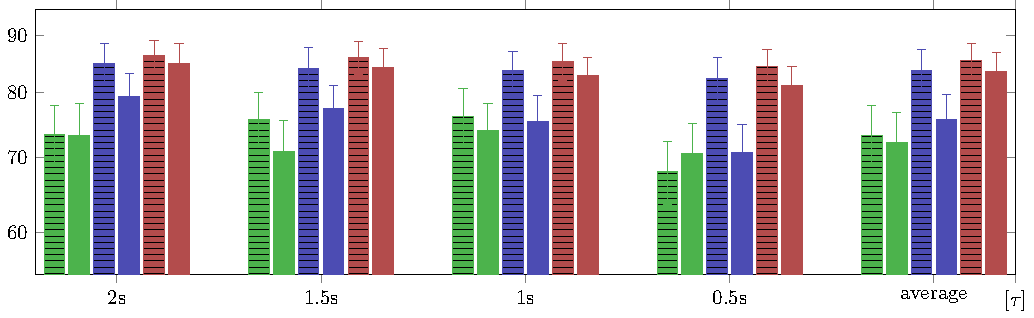
\includegraphics{Figures/Objective_1/acc_regularizacionHG_ME}}}\\
	\rotatebox{90}{\qquad \quad\, \textbf{DBIII-MI}}
	\rotatebox{90}{\qquad \quad\, \footnotesize{Accuracy ($\%$)}}
	{\resizebox{\kerrwidth}{!}{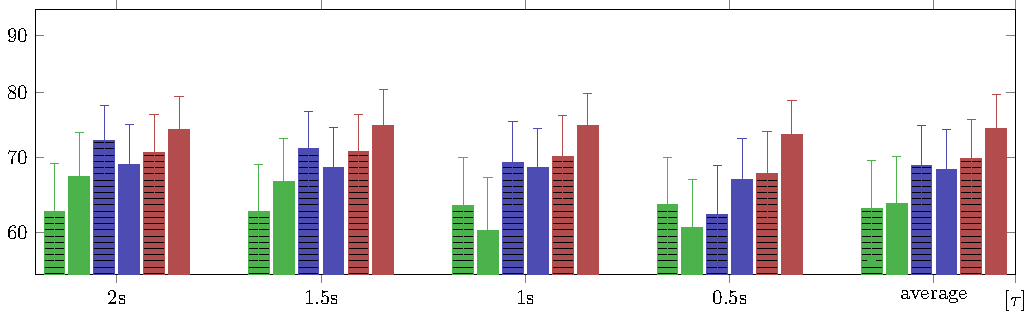
\includegraphics{Figures/Objective_1/acc_regularizacion}}} \\
	\hbox{\hspace{6cm} \textbf{Window length}}
	\caption{Accuracy performed at each $\tau$ by the evaluated measures of FC: PLV(\legend{green!40!gray}),~CCF(\legend{blue!40!gray}), and KCS-FC (\legend{red!40!gray}). {The full-filled colored bars stand for concatenate representation, while the bars with horizontal lines present the results after CSP filtering.}}\label{Fig:AccTau}
\end{figure}

At first sight, besides being distinctive from the CCF and GCF, the variability of accuracy estimates that are achieved by PLV (green line) becomes visible across the subject set of DBII ME: the shorter the window length, the more variable the subject estimates. Rather, the CCF and KCS-FC measures produce accuracy values following a similar order of subjects, for which the enhancing effect of CSP-based filtering can be observed. In the case of DBIII MI, the variability in classifier performance that is provided by the FC metrics grows noticeably, regardless of applying the CSP filtering. Thus, the order of subjects provided by each FC measure is particular and dissimilar to each other. Nevertheless, when compared with the baseline CCF-based accuracy (blue line), the proposed GCF measure without CSP allows for enhancing almost every single subject's discrimination ability, regardless of the window length applied. Moreover, the kernel-based FC measure ensures that several subjects exceed the BCI-inefficiency level, as previously assessed using CCF. It is noteworthy that using the CSP algorithm appreciably reduces the KCS-FC effectiveness for dealing with the subject variability of DBIII MI. 

\def \kerrwidth {0.44\linewidth} 
\begin{figure}[h!]
	\hbox{\hspace{3.3cm} \textbf{DBII-ME}\hspace{4.7cm} \textbf{DBIII-MI}}
	\rotatebox{90}{\qquad \,\footnotesize{Window size}}
	\rotatebox{90}{\qquad \, \footnotesize{$\tau= 2.0$\,{s}}}
	\rotatebox{90}{\qquad \,\tiny{Accuracy ($\%$)}}
	{\resizebox{\kerrwidth }{!}{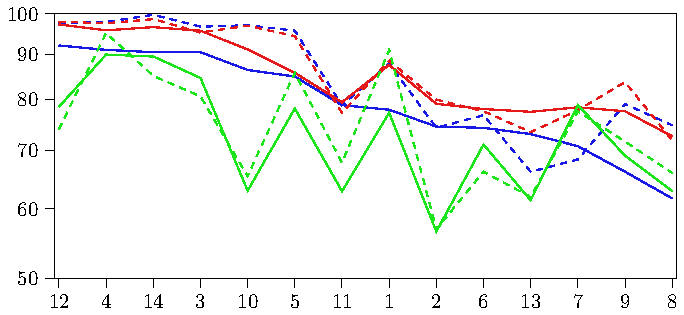
\includegraphics{Figures/Objective_1/ptau2-hg-Me}}}
	{\resizebox{\kerrwidth }{!}{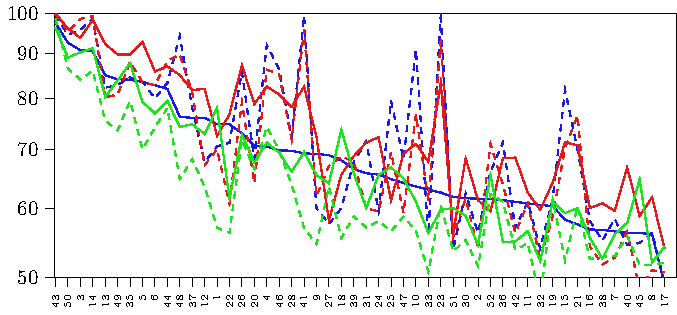
\includegraphics{Figures/Objective_1/ptau2-giga-Mi}}} \\
	\rotatebox{90}{\qquad \,\footnotesize{Window size}}	
	\rotatebox{90}{\qquad \, \footnotesize{$\tau= 1.5$\,{s}}}
	\rotatebox{90}{\qquad \,\tiny{Accuracy ($\%$)}}
	{\resizebox{\kerrwidth }{!}{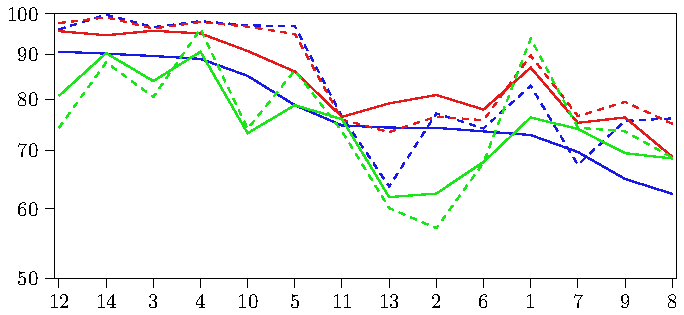
\includegraphics{Figures/Objective_1/ptau1_5-hg-Me}}}
	{\resizebox{\kerrwidth }{!}{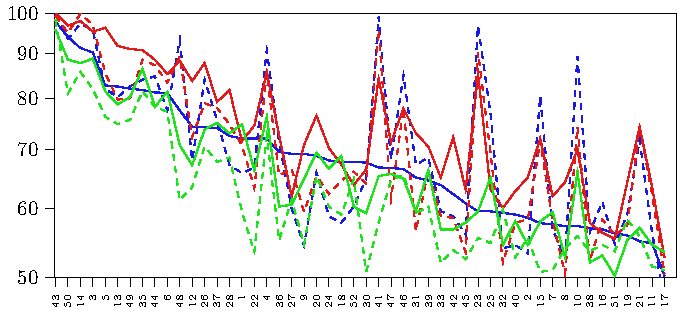
\includegraphics{Figures/Objective_1/ptau1_5-giga-Mi}}}\\
	\rotatebox{90}{\qquad \,\footnotesize{Window size}}	
	\rotatebox{90}{\qquad \, \footnotesize{$\tau= 1.0$\,{s}}}
	\rotatebox{90}{\qquad \,\tiny{Accuracy ($\%$)}}
	{\resizebox{\kerrwidth }{!}{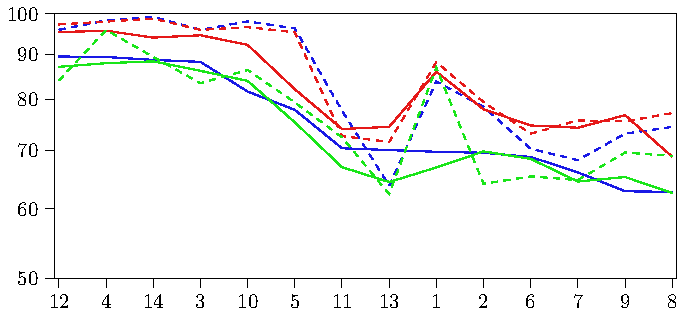
\includegraphics{Figures/Objective_1/ptau1-hg-Me}}}
	{\resizebox{\kerrwidth }{!}{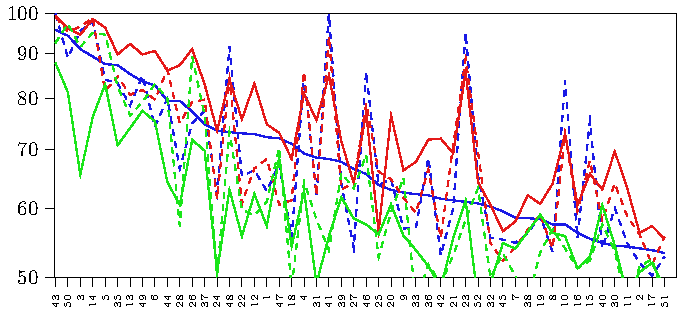
\includegraphics{Figures/Objective_1/ptau1-giga-Mi}}}\\
	\rotatebox{90}{\qquad \,\footnotesize{Window size}}	
	\rotatebox{90}{\qquad \, \footnotesize{$\tau= 0.5$\,{s}}}
	\rotatebox{90}{\qquad \,\tiny{Accuracy ($\%$)}}
	{\resizebox{\kerrwidth }{!}{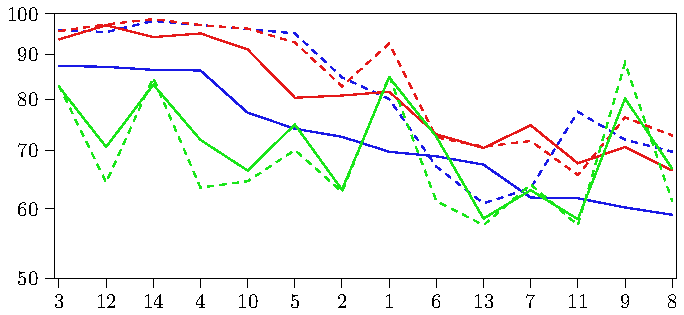
\includegraphics{Figures/Objective_1/ptau0_5-hg-Me}}}
	{\resizebox{\kerrwidth }{!}{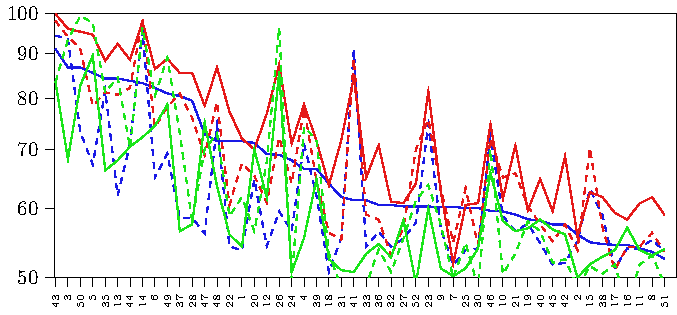
\includegraphics{Figures/Objective_1/ptau0_5-giga-Mi}}} \\
	\hbox{\hspace{3.3cm} \footnotesize{Subject id}\hspace{5.1cm} \footnotesize{Subject id}}
	\caption{Individual classifier performance at different window lengths using FC: PLV (${\lineplot{color5}}$), CCF (${\lineplot{color1}}$), and KCS-FC (${\lineplot{color3}}$). The accuracy assessments performed without CSP are outlined with a continuous line, after CSP filtering---with a dashed line. The subjects are displayed on the horizontal axis in decreasing order of their CCF-based accuracy.}
	\label{Fig:IndividualAcc}
\end{figure}

\subsection{Interpretation of Subject Clusters Using Functional Connectivity Patterns}

The main goal can be framed as the grouping of subjects having similar spatial networks involved in the motor-related tasks under consideration, aiming to properly interpret the evaluated functional connectivity measures. {To this end, we cluster the extracted FC sets into partitions, each one with resembling subjects in terms of FC dynamics, being coded in the relevance vector $\ve{v}$ of Equation~\eqref{eq:SRC}, and the motor-related accuracy. However, because of the poor clustering performance in high dimensional spaces, we accomplish a previous dimensional reduction stage on the normalized subject's relevance vector set (fixing a 2D low-dimensionality) through t-Distributed Stochastic Neighbor Embedding (t-SNE), which preserves the spatial relationships in the higher space (nearest-neighbors)~\cite{linderman2019clustering}. Subsequently, we concatenate the t-SNE low-dimensional representation with the corresponding individual accuracy to perform a {k}-means-based clustering. At each window length, the latter approach is carried out, as proposed in~\cite{Kim2019}.}

One concern is how a subject may switch between the assigned clusters when accounting for the influence of extracted FC measures at each window length. To clarify this aspect, Figure \ref{Fig:clust} displays the clustering results achieved by each functional connectivity measure using a matrix that illustrates the cells colored according to the individual group assessed, ranking the assessed groups in decreasing order of accuracy averaged over the corresponding subset. The three groups are colored, as follows: Group I, giving the best accuracy I (in yellow), Group II with regular accuracy (purple), and Group III, performing the worst accuracy (Turquoise).

\def \kerrwidthME {.32\linewidth}
\def \kerrwidthMI {.55\linewidth}
\begin{figure}[h!]	
\centering
	\hbox{\hspace{2.1cm} \textbf{DBII~ME}\hspace{5cm} \textbf{DBIII~MI}}
	\rotatebox{90}{\qquad {PLV}} 
	\rotatebox{90}{\quad \,\footnotesize{Window size}}	
	{\resizebox{\kerrwidthME}{!}{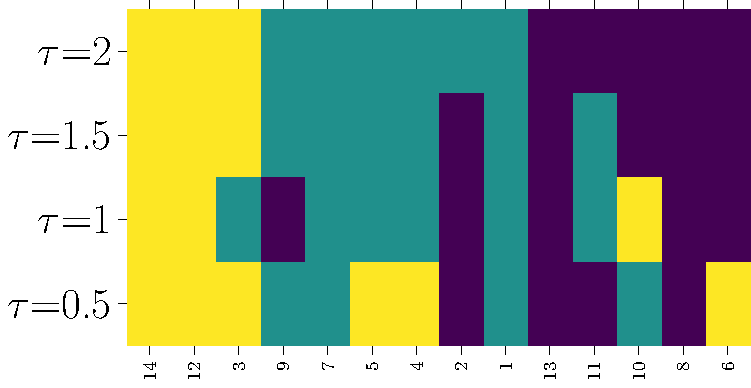
\includegraphics{Figures/Objective_1/plv_hg}}}
	{\resizebox{\kerrwidthMI}{!}{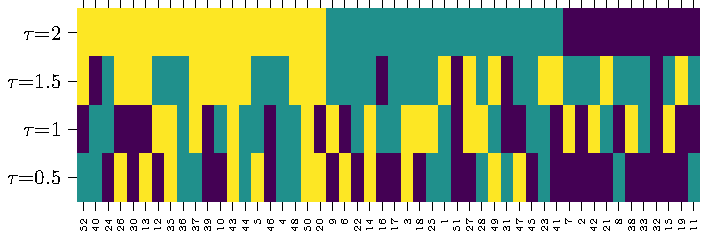
\includegraphics{Figures/Objective_1/plv_giga}}}\\
	\rotatebox{90}{\qquad {CCF}} 
	\rotatebox{90}{\quad \,\footnotesize{Window size}}		
	{\resizebox{\kerrwidthME}{!}{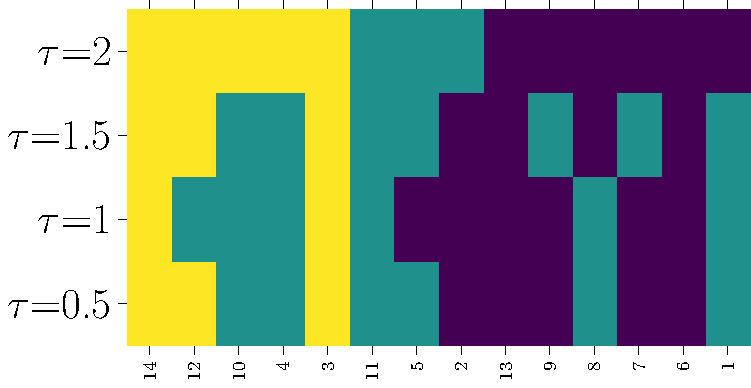
\includegraphics{Figures/Objective_1/pearson_hg}}}
	{\resizebox{\kerrwidthMI}{!}{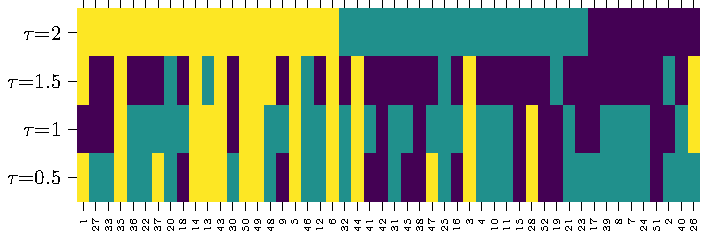
\includegraphics{Figures/Objective_1/pearson_giga}}}\\
	\rotatebox{90}{\qquad {KCS-FC}} 
	\rotatebox{90}{\quad \,\footnotesize{Window size}}		
	{\resizebox{\kerrwidthME}{!}{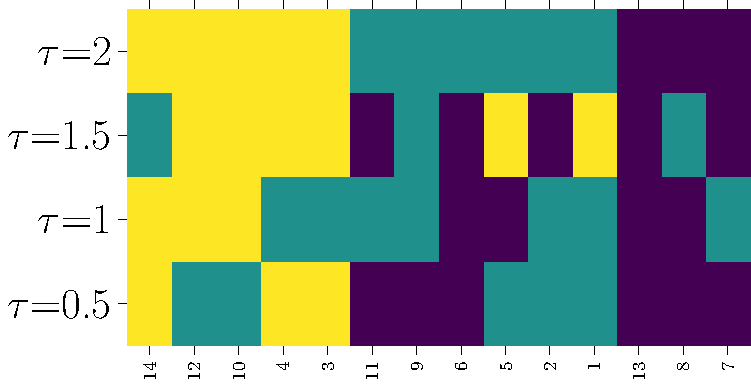
\includegraphics{Figures/Objective_1/gauss_hg}}}
	{\resizebox{\kerrwidthMI}{!}{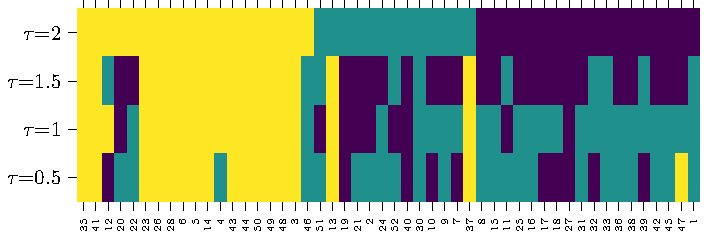
\includegraphics{Figures/Objective_1/gauss_giga}}}\\
	\hbox{\hspace{2.1cm} \footnotesize{Subject id}\hspace{5cm} \footnotesize{Subject id}}
	\caption{Clustering variability of individuals that belong to Group I (cells in yellow), {Group II (Turquoise), and Group III (purple)}, depending on the extracting window length $\tau$.} \label{Fig:clust}	
\end{figure} 

{As seen for DBII ME, the intragroup similarity remains comparable in groups I and III over the values of $\tau$, while Group II has noticeable volatile behavior}. This result may be explained because of the low number of database subjects (only 14), making any exchange seriously affect the intergroup distribution. In DBIII MI, the high subject variability that is reflected by the functional connectivity extracted yields high changeability between groups, at least for the PLV and CCF measures. Rather, the proposed KCS-FC measure is less affected, as seen at window values of $2$ and $1.5$\,{s}. Further, groups II and III become scrambled, meaning that the subject variability extracted at the shorter window lengths remains hard to overcome. 

The last aspect of the study is the interpretability of motor-related tasks as reliable sources of neural responses in the assessed clusters of dynamic behavior (the groups are denoted as I, II, and III).

{\Cref{Fig:Topograms} presents the topographic channel plots (topoplots) that contain the relevant activated scalp areas that are inferred from the extracted FC measures, principally contributing to the discriminability between labeled motor-related tasks. We also include the most relevant pairwise functional connectivity links between electrodes that are estimated to fulfill the $99$ percentile of the normalized relevance weights values (between 0 to 1) computed from Equation~\eqref{eq:SRC}. The background stands for the accumulated relevance that is mapped to the channel positions.} In DBII ME, only the SMR area is depicted according to the electrode set configuration above-described. 

PLV performs in DBII ME the first three plots in the top row. The topoplots reflect high evoked response amplitudes that are densely spread over the SMR area, which means that the PLV variability hampers the sparse feature selection framework to obtain a reduced set of extracted FC features. Still, a few links surpass the $99$ percentile, which enables some information regarding the relevant electrodes. Contrary to this, the three topoplots that are delivered by CCF (middle row) and KCS-FC (bottom row) show low amplitudes of neural activity in Group I, slightly increased activity of Group II, and increased amplitudes of the worst-performing group of individuals (III). However, the latter FC measure clearly shows two foci that are symmetrically located over each hemisphere, as expected in motor-related tasks, at least for GI and, to a less extent, for GII. Besides, the amount of relevant links estimated is low. Consequently, the sparse-based $\ell_2$-norm framework enables the effective dimensionality reduction of the extracted KCS-FC features. Moreover, the accuracy using KCS-FC assessed by every group of individuals outperforms the other compared functional connectivity metrics: PLV and CCF. 

\nointerlineskip
\def \kerrwidth {0.15\linewidth}
\def \kerrwidthc {0.022\linewidth}
\def \kerrg {0.12\linewidth}
\def \kerrgg {0.05\linewidth}
\def \kerrggg {0.04\linewidth}
%\begingroup
\tabcolsep = 2.0pt
\def\arraystretch{1.0}
\begin{figure}[h!]
%\widefigure
\scalebox{0.95}[0.95]{\begin{tabular}{cccccccc}
\centering
& & \textbf{DBII~ME}& & & \textbf{DBIII~MI}&\\
\cmidrule{2-7}
& {I} & {II}&{III}&{I} & {II}&{III}&
\multirow{6}{*}{{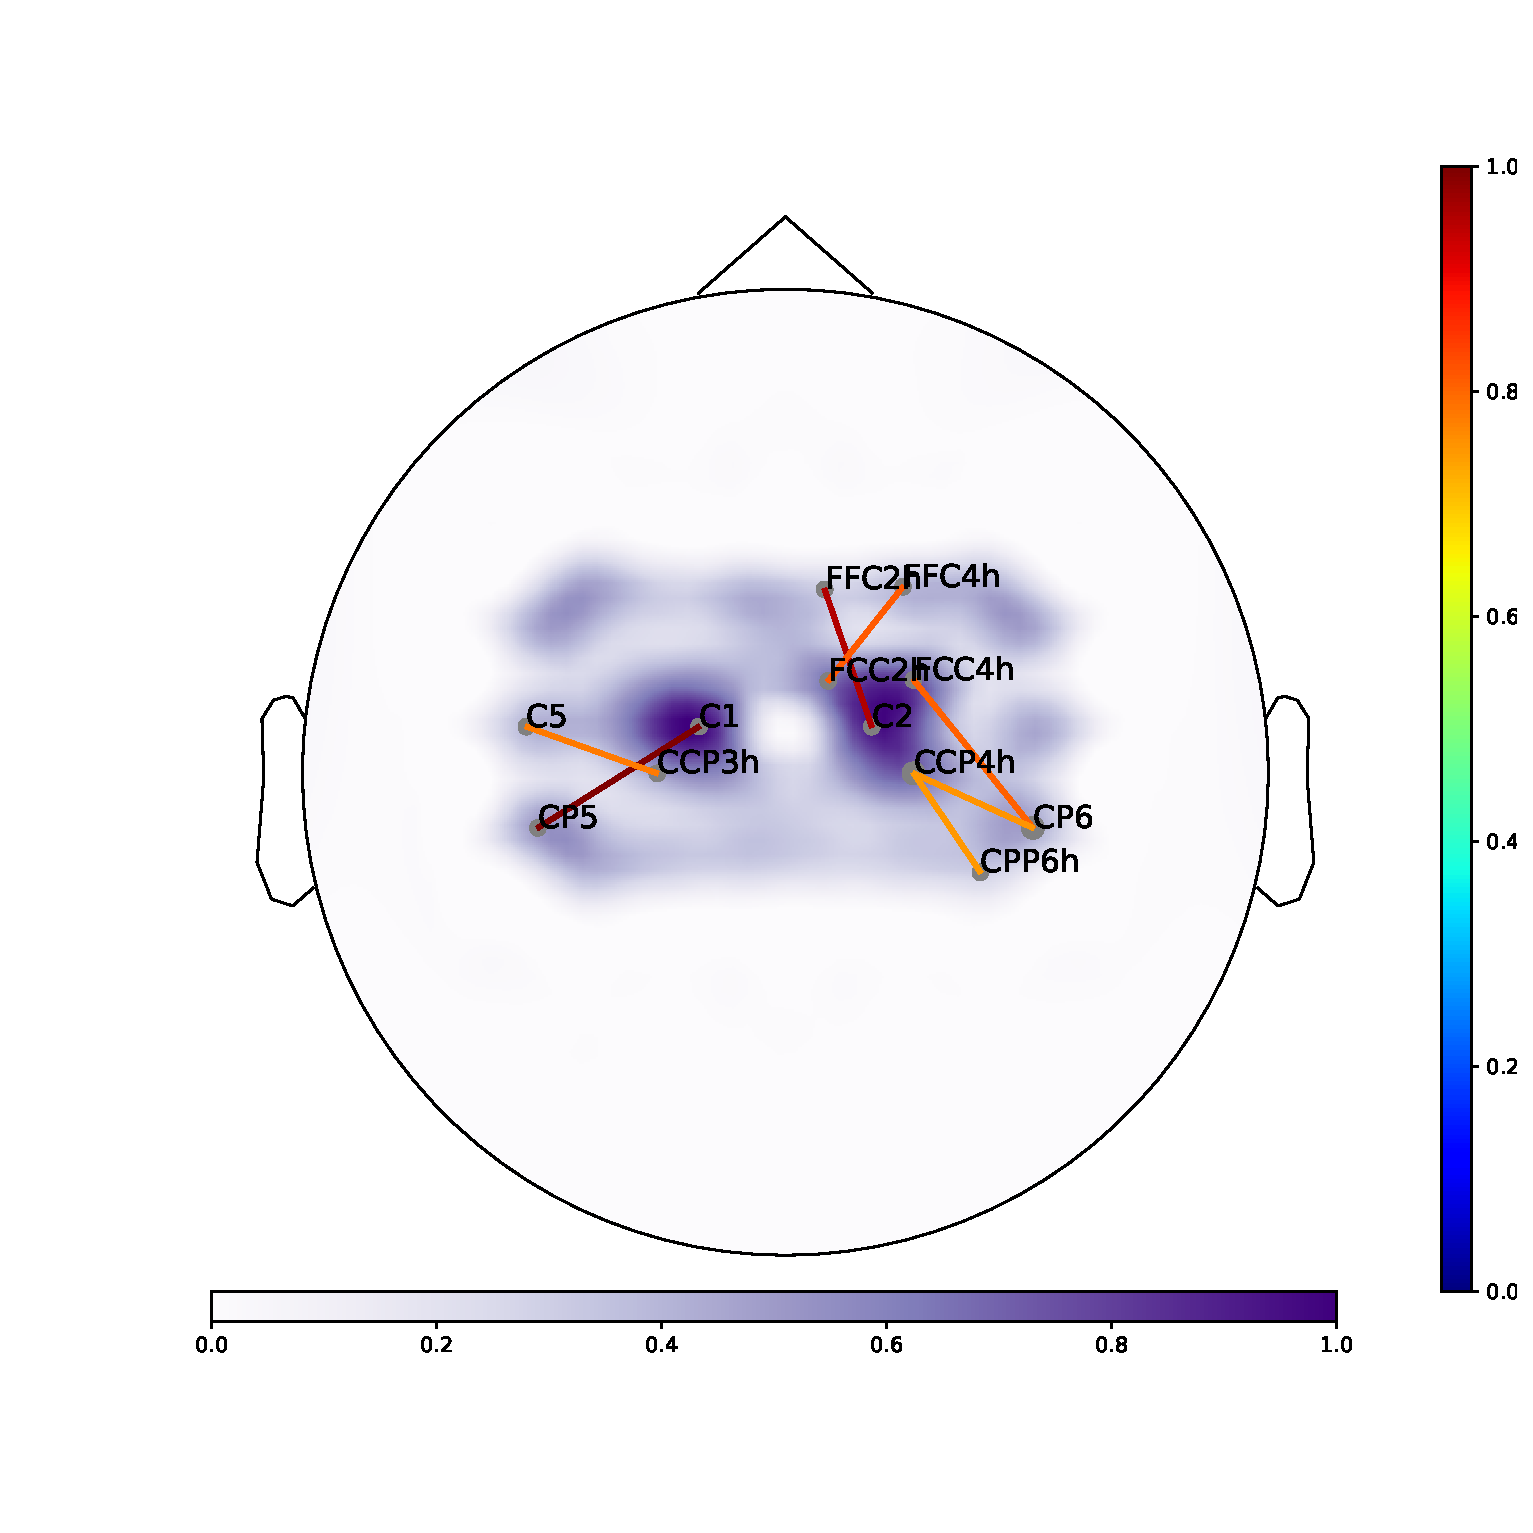
\includegraphics[trim=660 0 0 0, clip,scale=0.35]{Figures/Objective_1/Cxsbj1hg-gaussacc95.28.eps}}}\\
\cmidrule{2-7}
& \textbf{$84.13\%$}& \textbf{$74.91\%$} & \textbf{$64.21\%$} & \textbf{$72.2\%$} & \textbf{$68.76\%$} & \textbf{$55.94\%$}&\\
{\rotatebox{90}{\hspace{7mm} {PLV}}}&{\resizebox{\kerrwidth}{!}{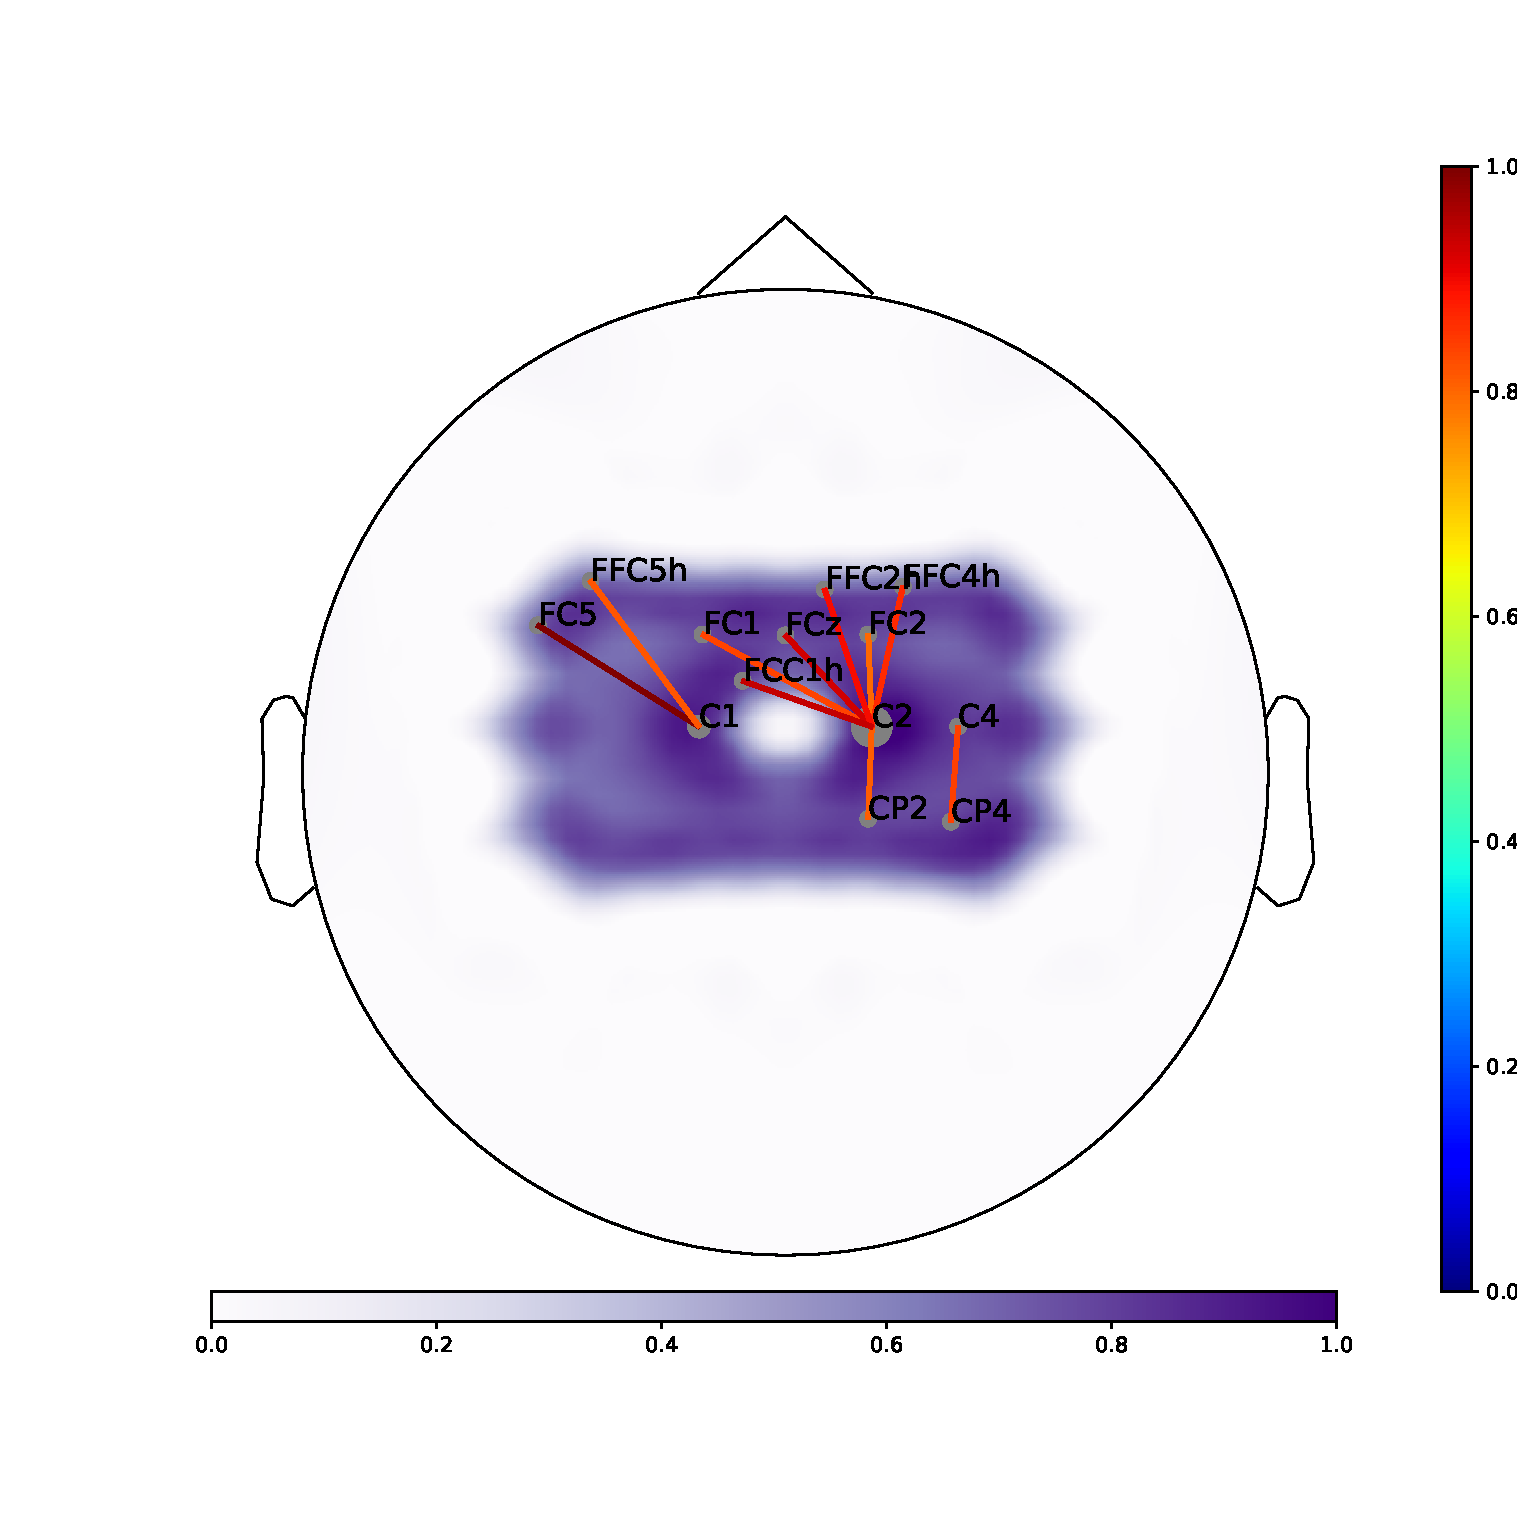
\includegraphics[trim=100 120 90 90, clip]{Figures/Objective_1/Cxsbj1hg-plvacc84.13.eps}}}&
	{\resizebox{\kerrwidth}{!}{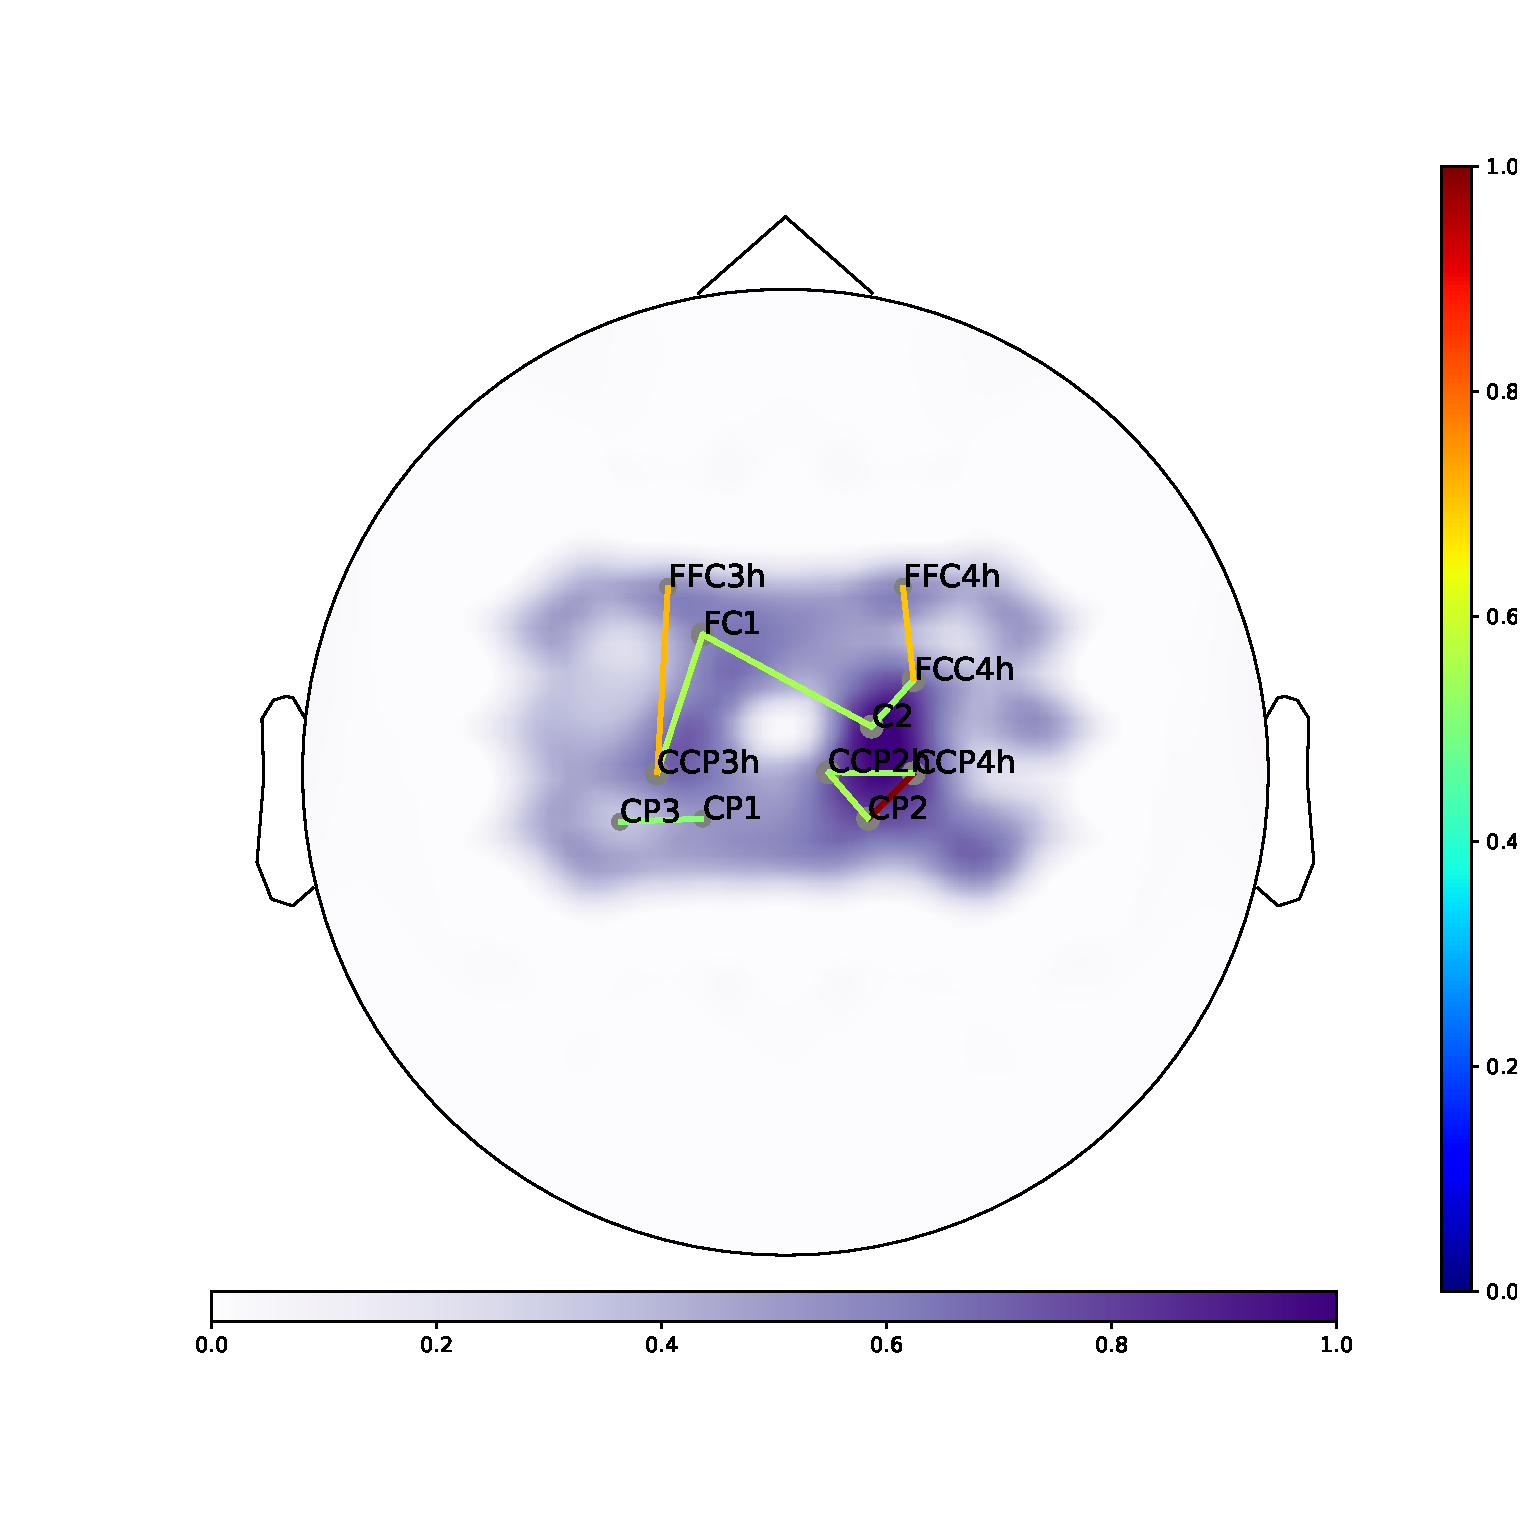
\includegraphics[trim=100 120 90 90, clip]{Figures/Objective_1/Cxsbj2hg-plvacc74.91.eps}}}&
	{\resizebox{\kerrwidth}{!}{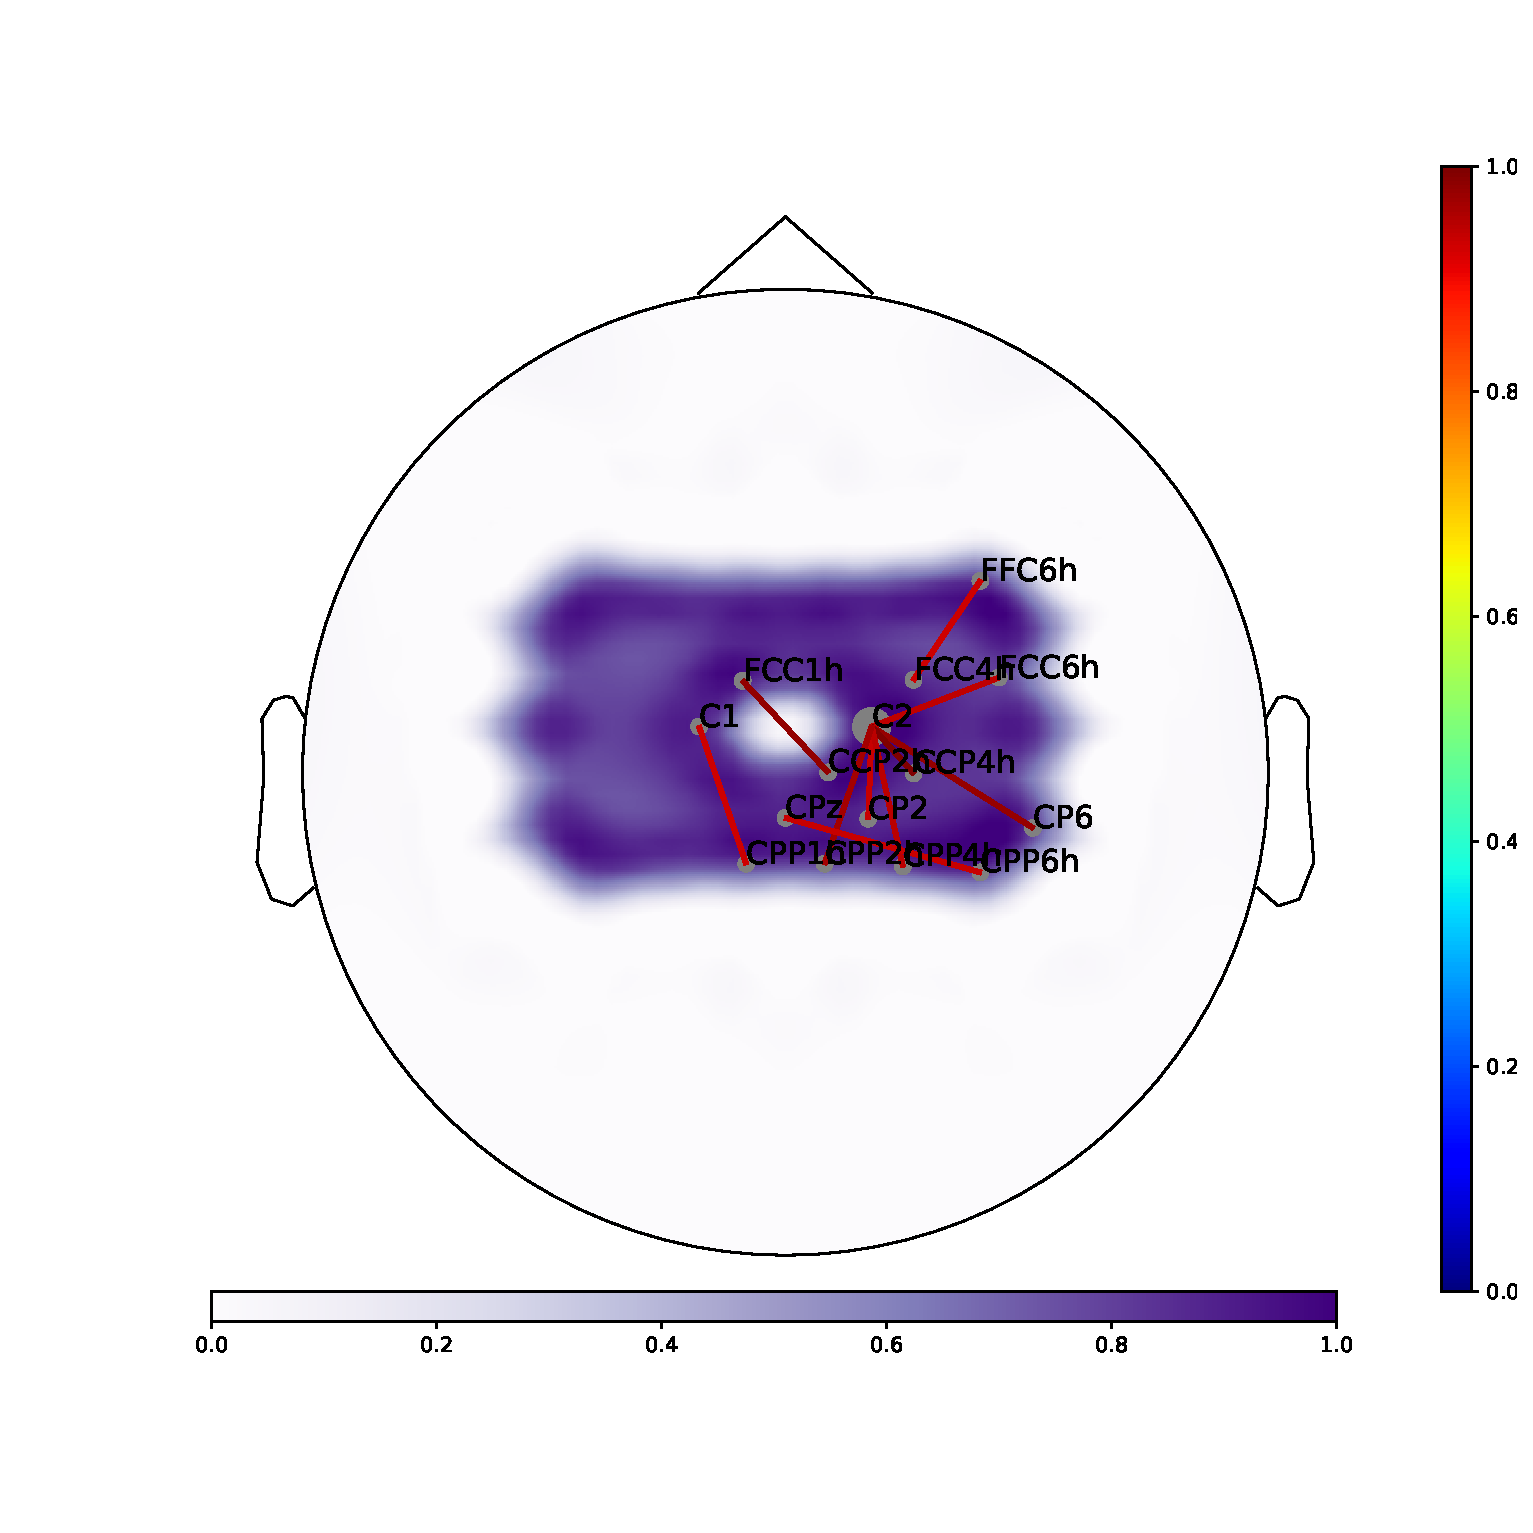
\includegraphics[trim=100 120 90 90, clip]{Figures/Objective_1/Cxsbj3hg-plvacc64.21.eps}}}&
	{\resizebox{\kerrwidth}{!}{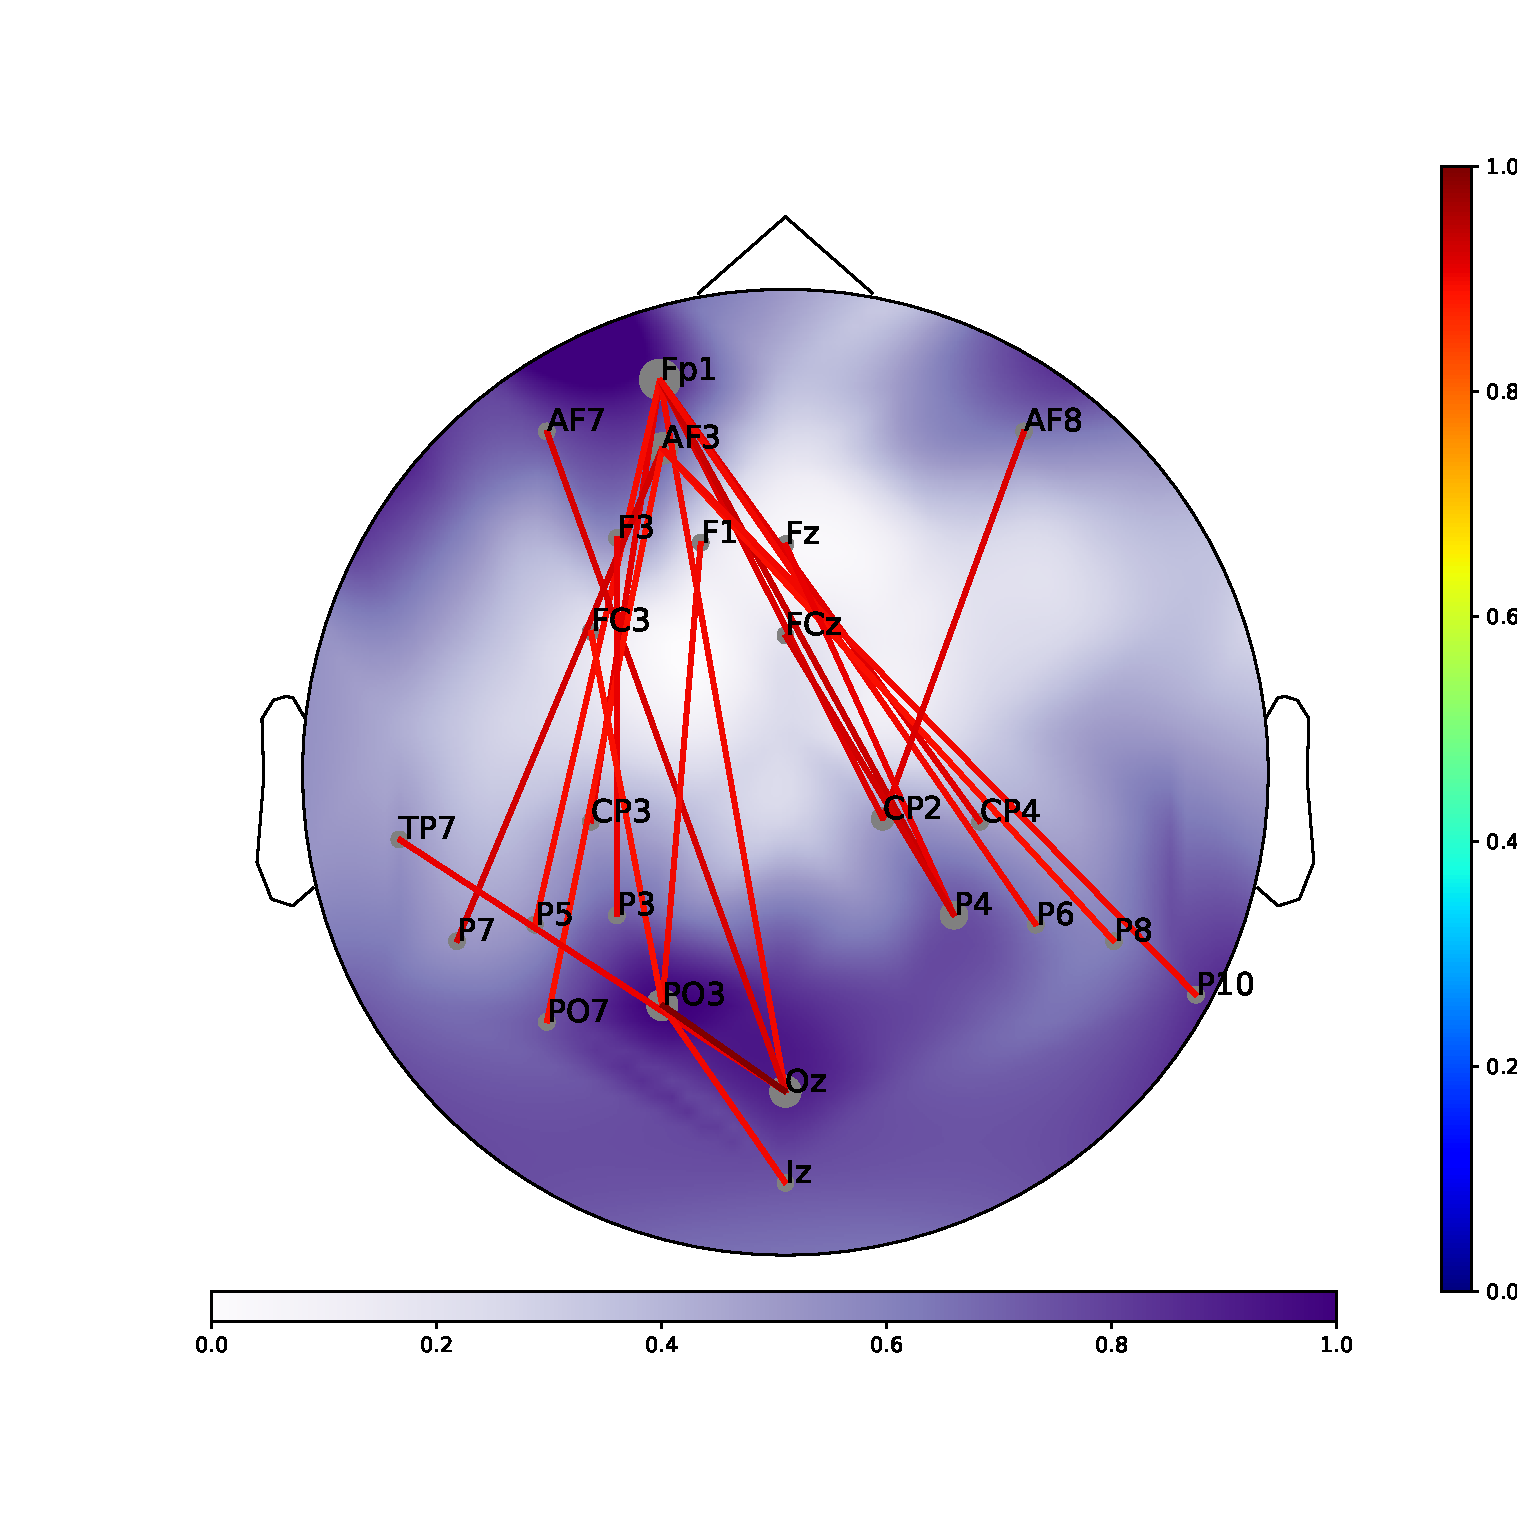
\includegraphics[trim=100 120 90 90, clip]{Figures/Objective_1/Cxsbj1plvacc72.2.eps}}}&
	{\resizebox{\kerrwidth}{!}{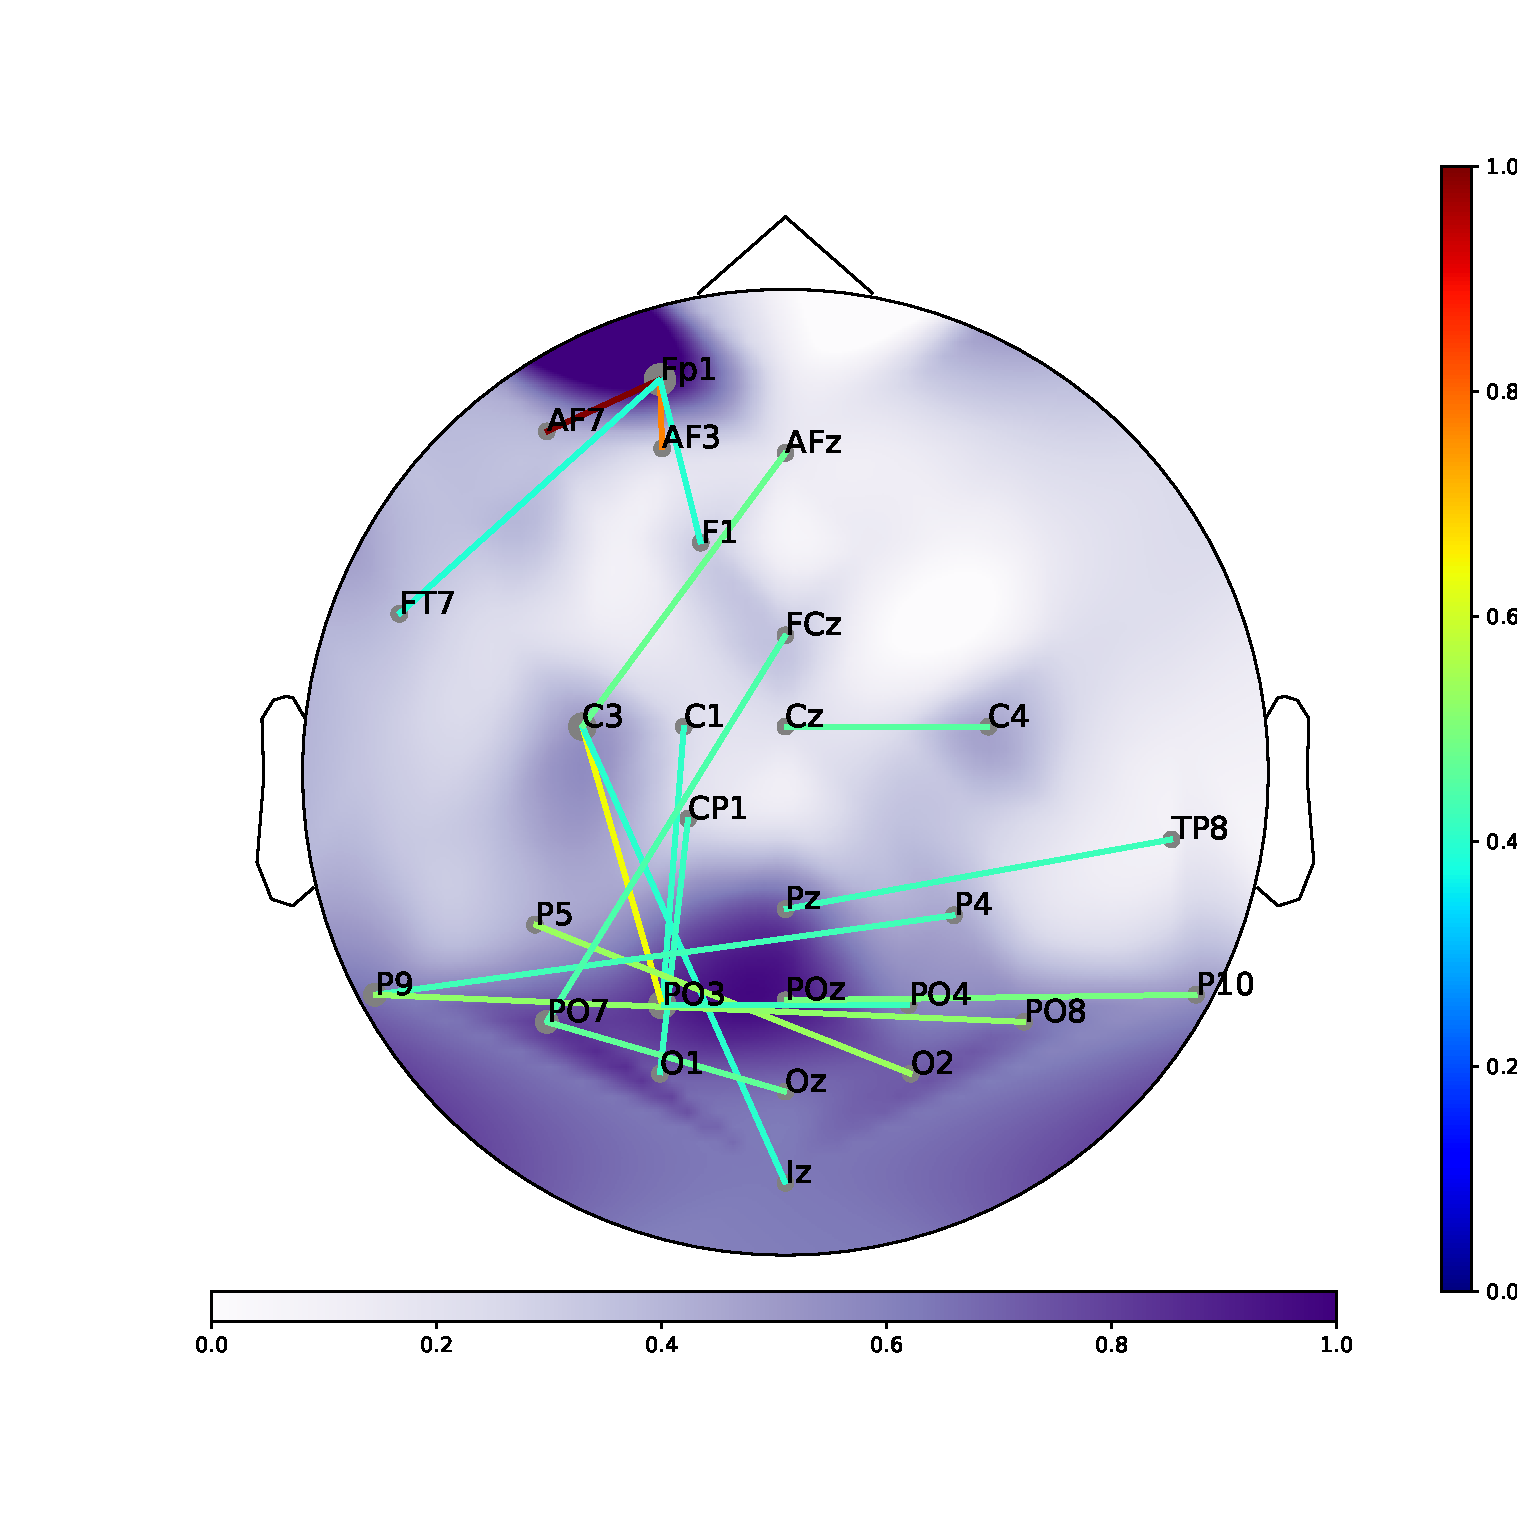
\includegraphics[trim=100 120 90 90, clip]{Figures/Objective_1/Cxsbj2plvacc68.76.eps}}}&
	{\resizebox{\kerrwidth}{!}{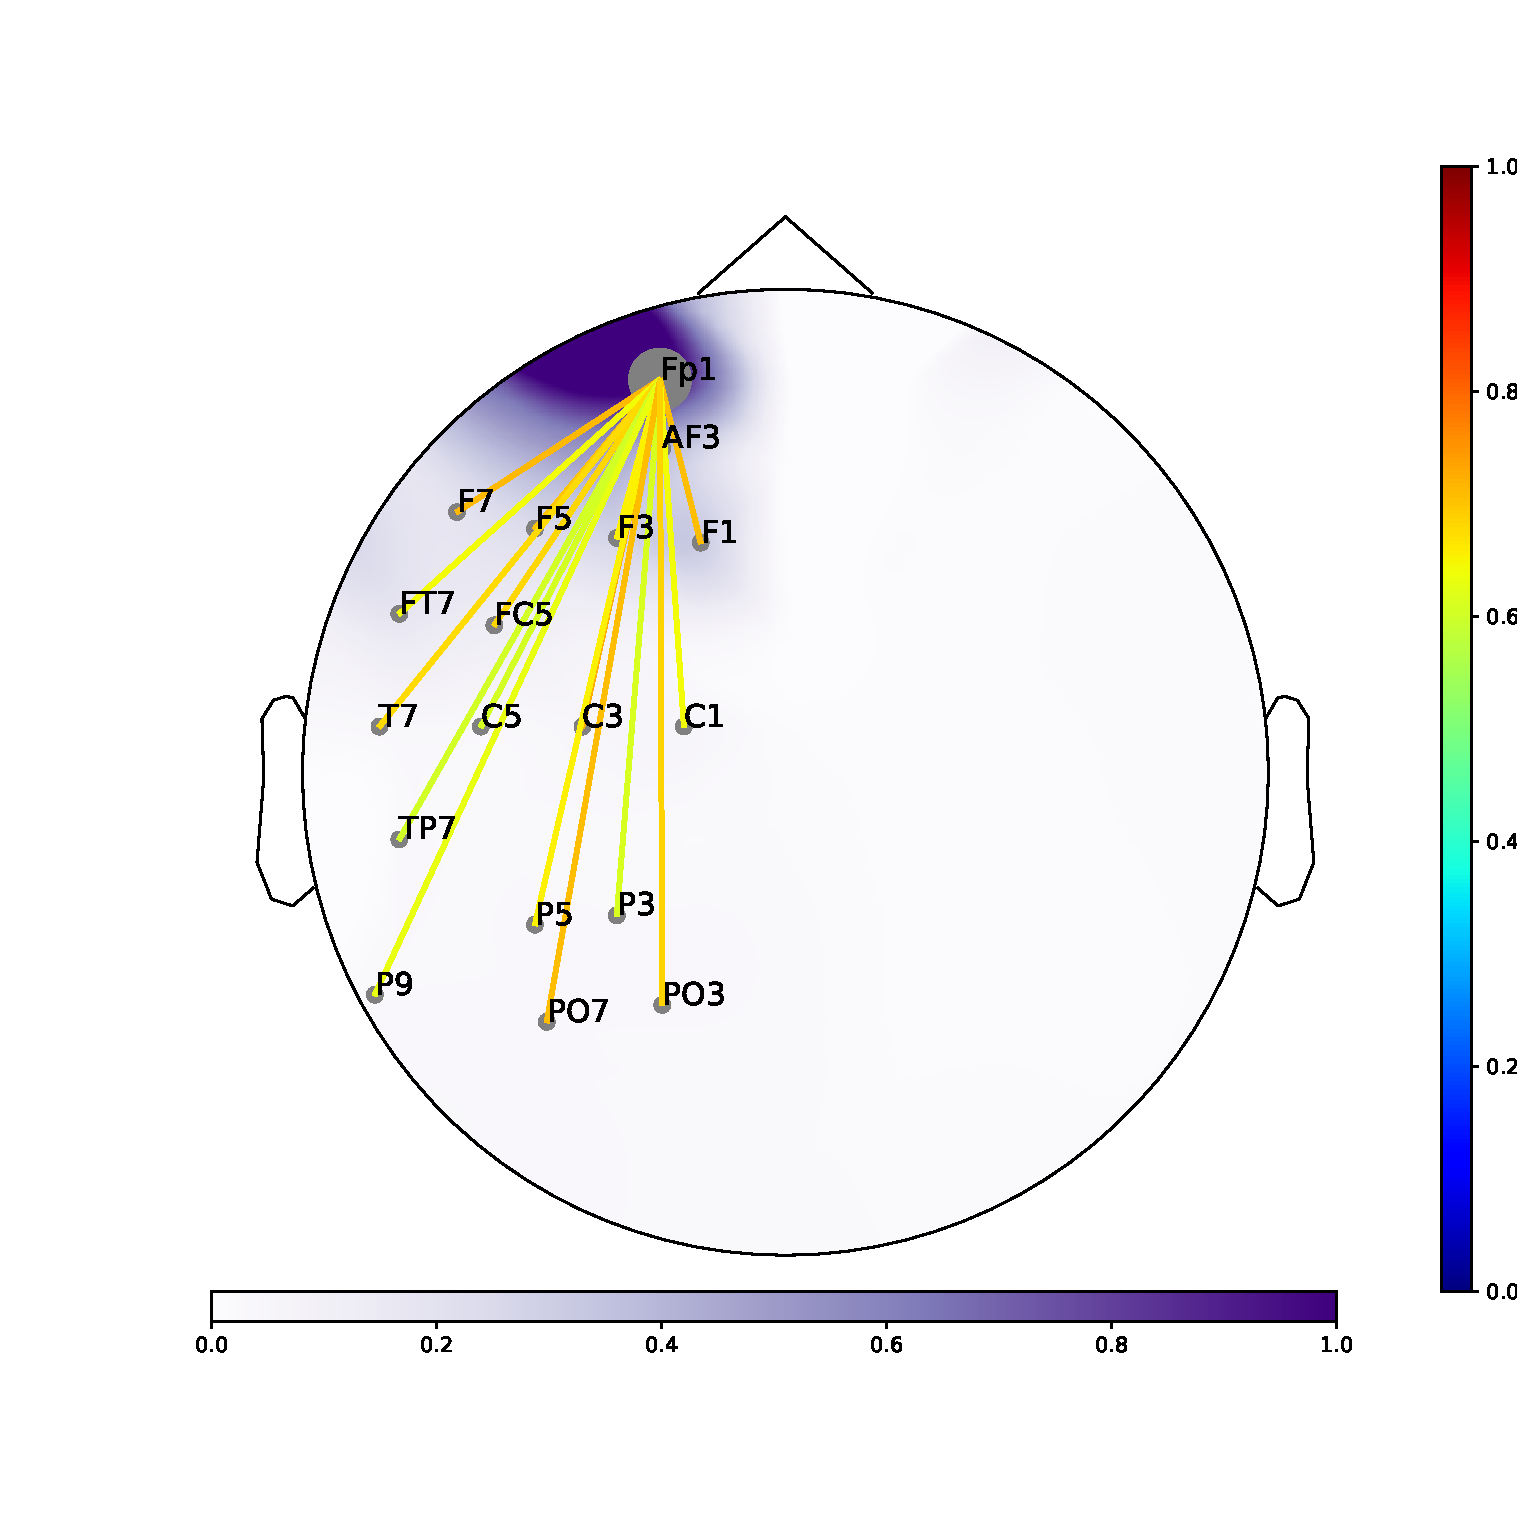
\includegraphics[trim=100 120 90 90, clip]{Figures/Objective_1/Cxsbj3plvacc55.94.eps}}}&\\
	& \textbf{$90.06\%$} & \textbf{$79.35\%$} & \textbf{$70.59\%$} &  \textbf{$76.67\%$} & \textbf{$64.62\%$} & \textbf{$60.69\%$}&\\
	\rotatebox{90}{\hspace{7mm} {CCF}}&
	{\resizebox{\kerrwidth}{!}{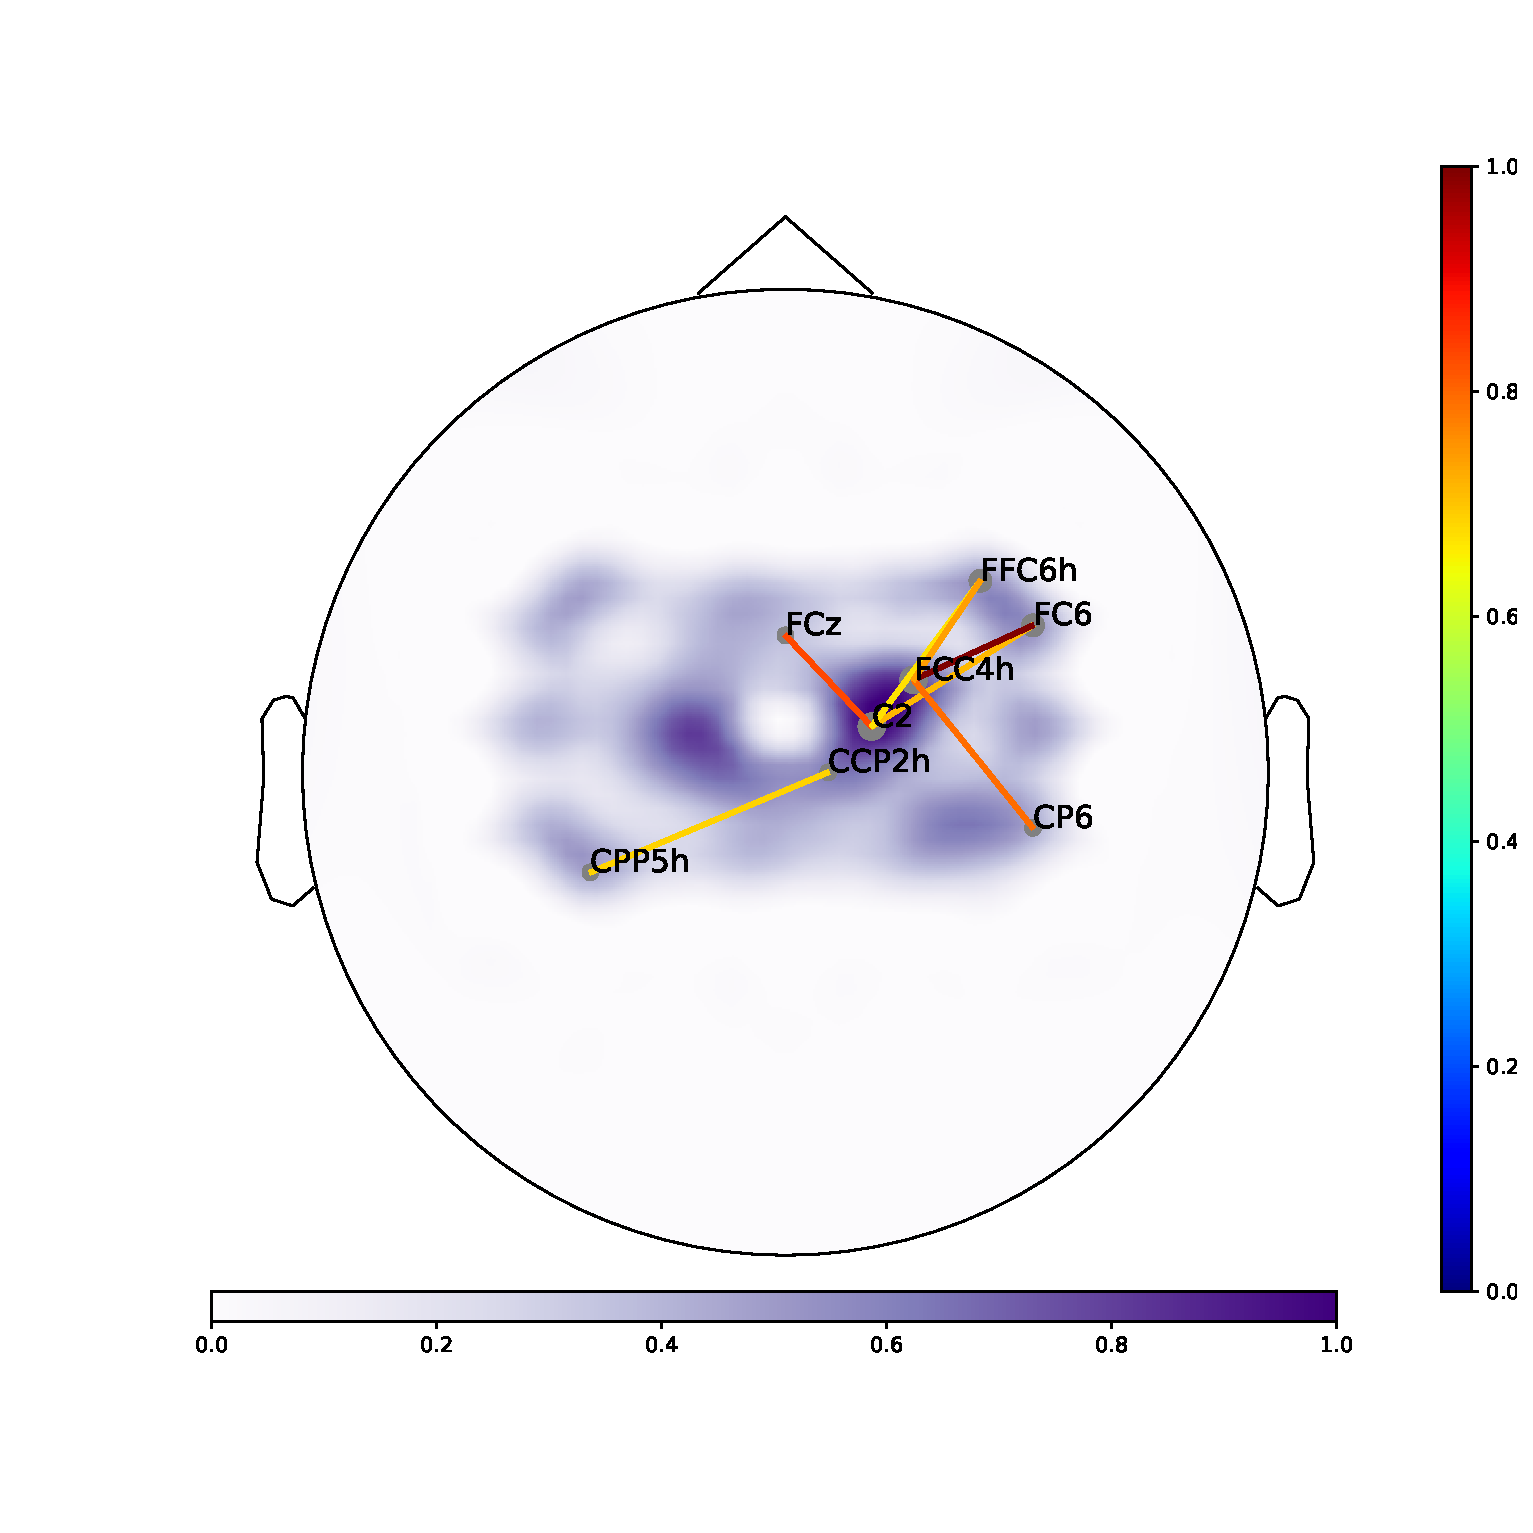
\includegraphics[trim=100 120 90 90, clip]{Figures/Objective_1/Cxsbj1hg-pearsonacc90.06.eps}}}&
	{\resizebox{\kerrwidth}{!}{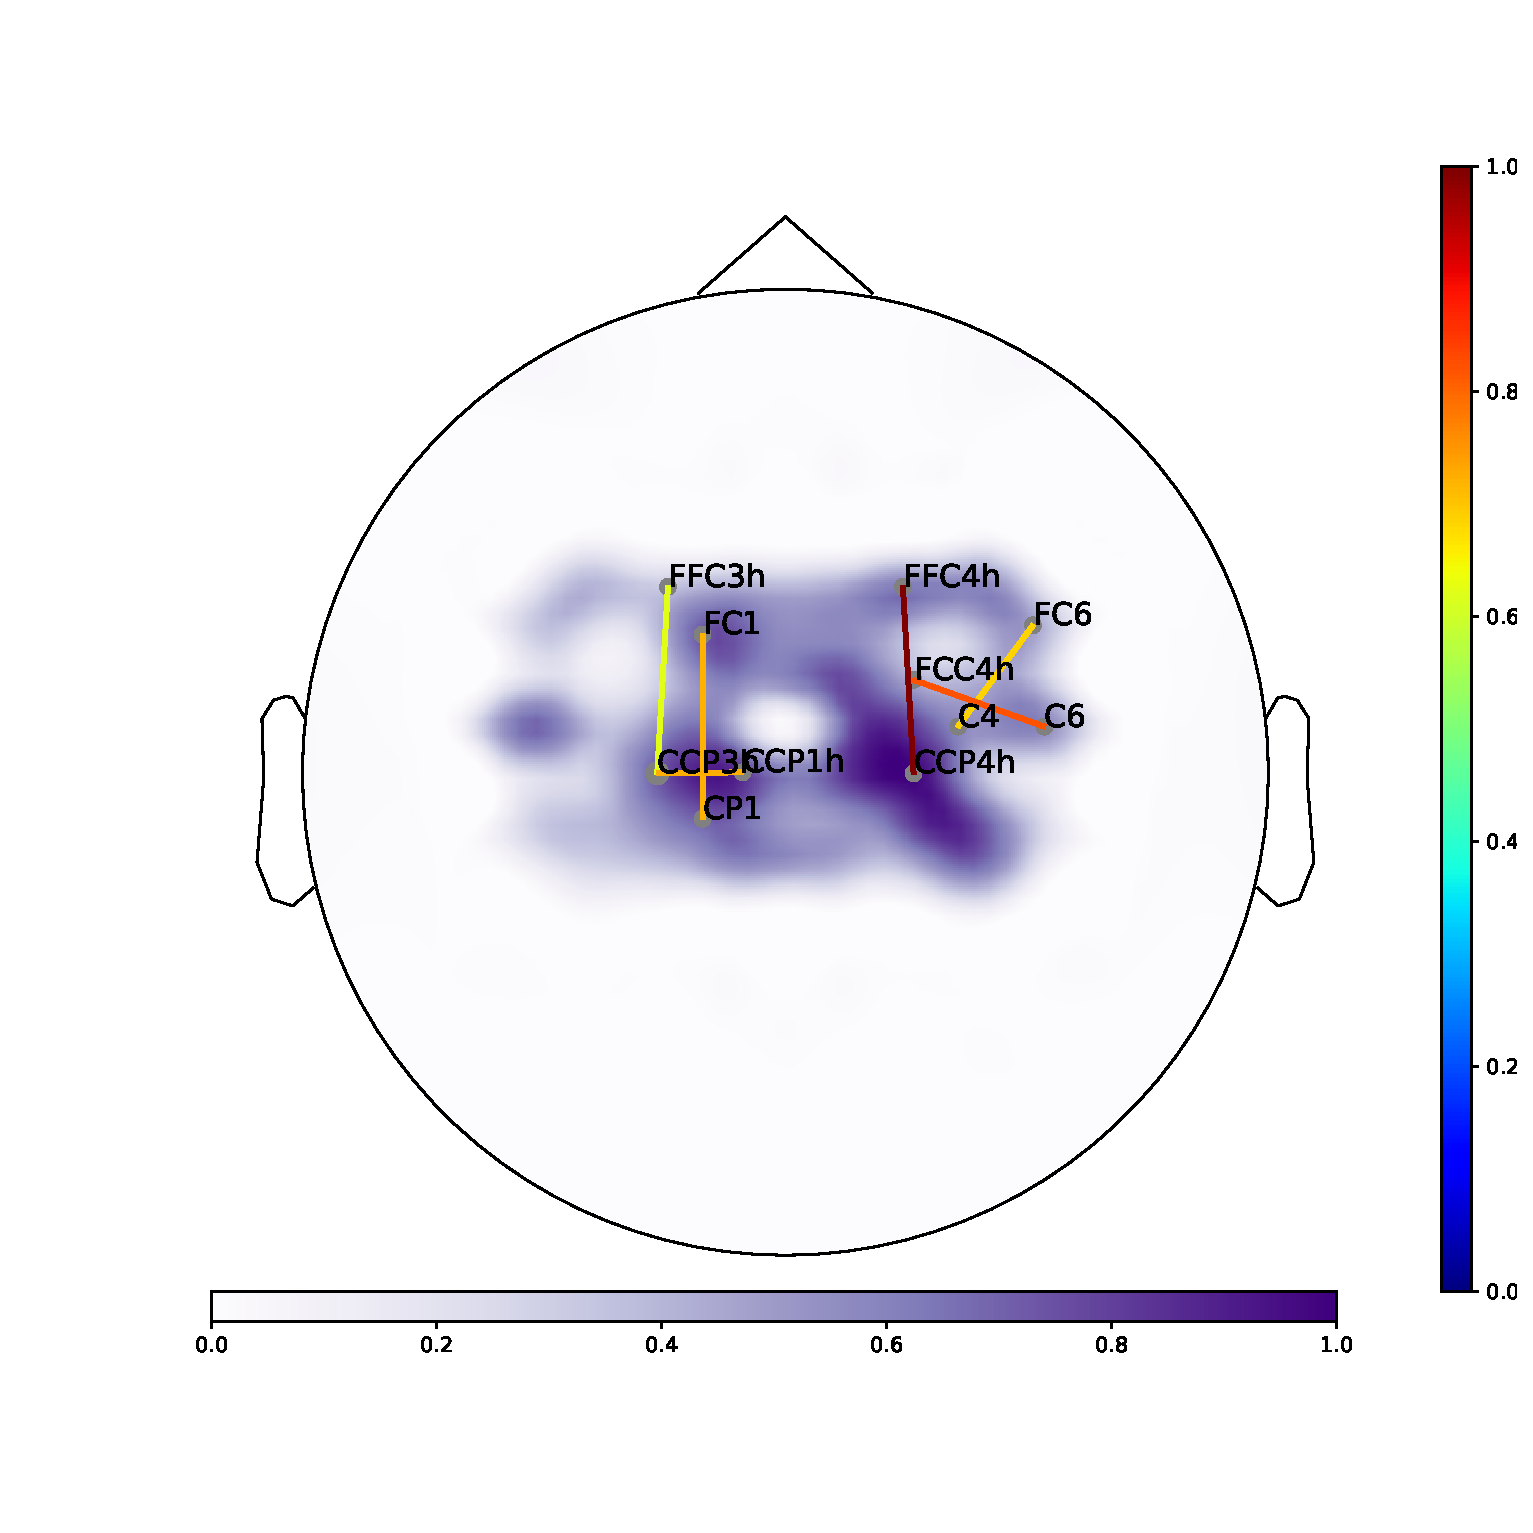
\includegraphics[trim=100 120 90 90, clip]{Figures/Objective_1/Cxsbj2hg-pearsonacc79.35.eps}}}&
	{\resizebox{\kerrwidth}{!}{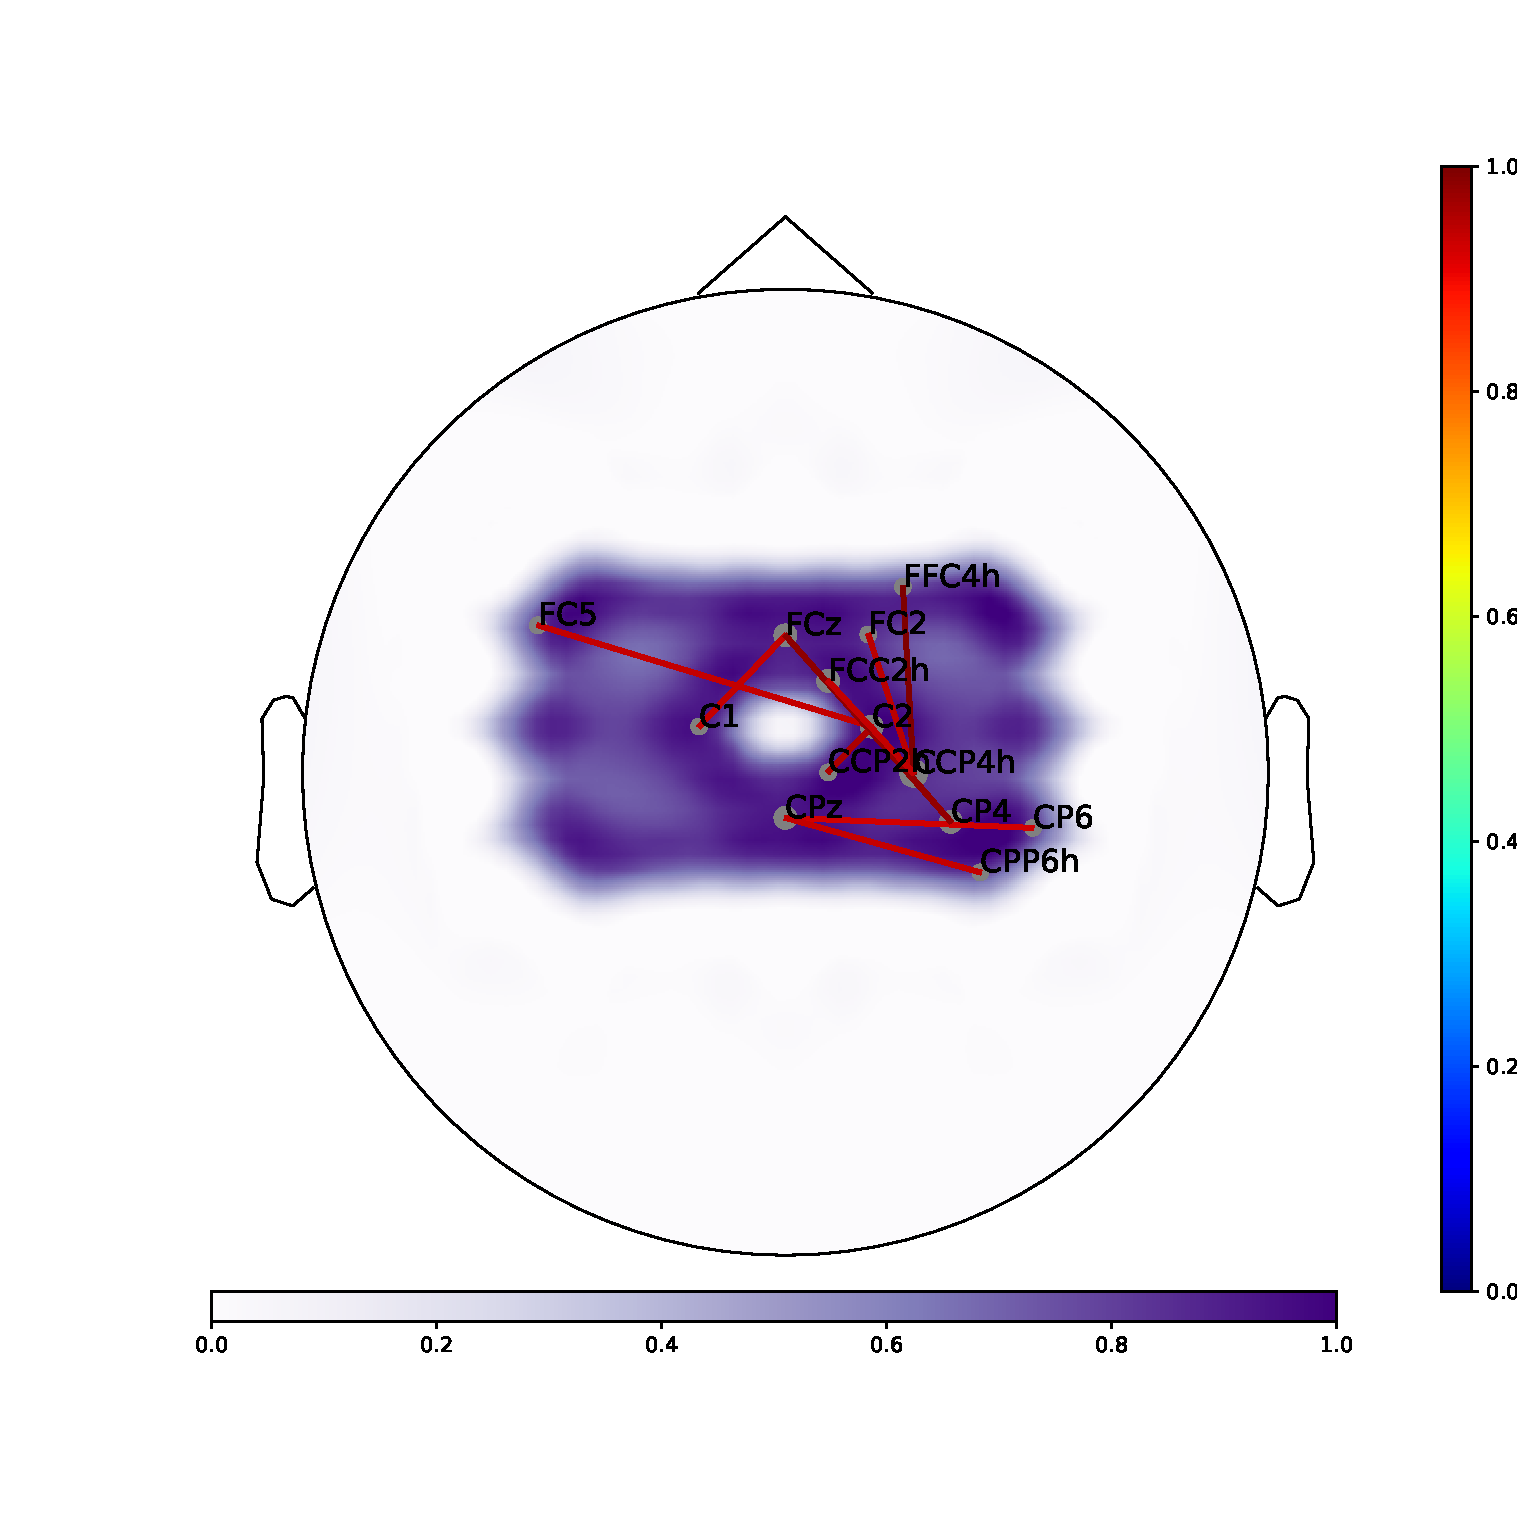
\includegraphics[trim=100 120 90 90, clip]{Figures/Objective_1/Cxsbj3hg-pearsonacc70.59.eps}}}&
	{\resizebox{\kerrwidth}{!}{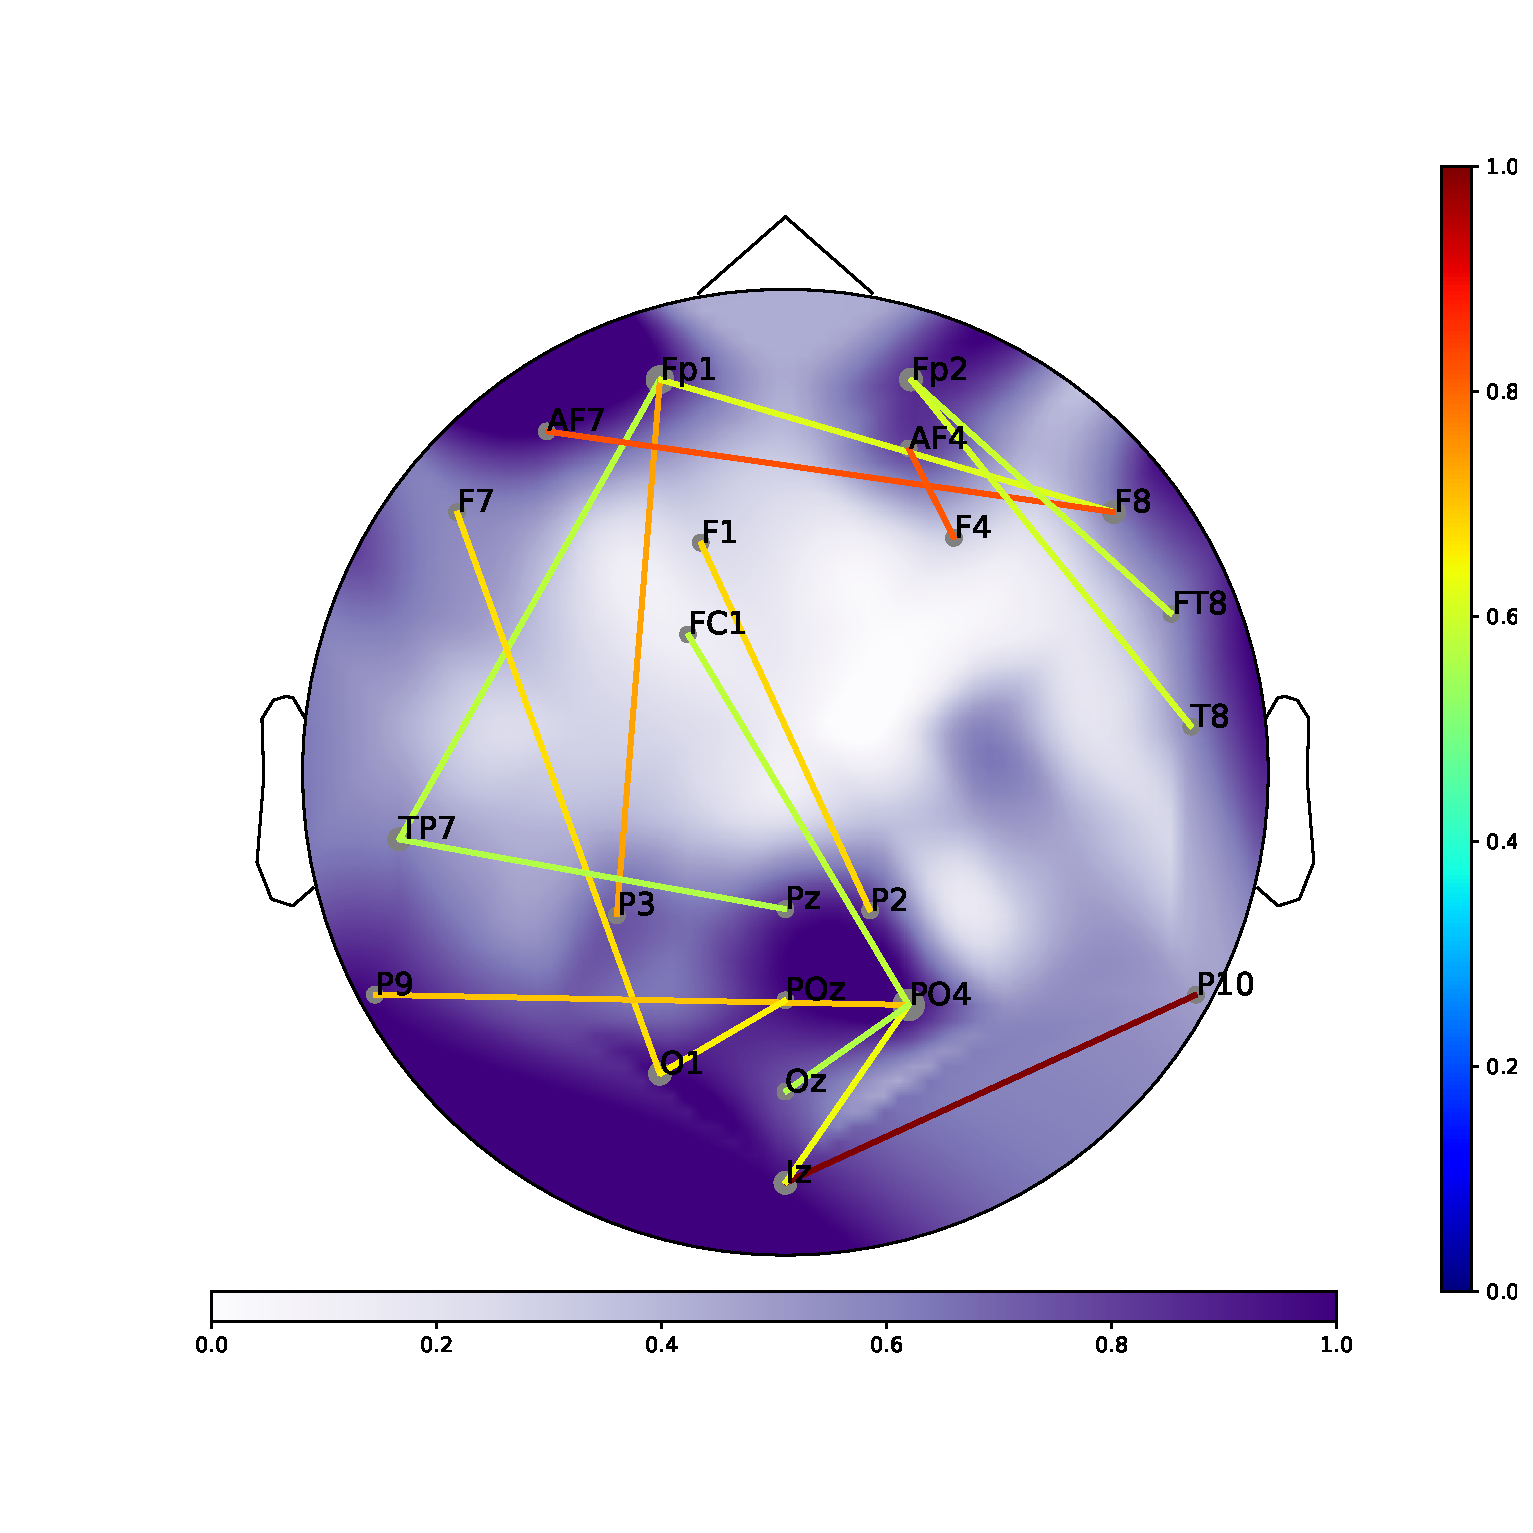
\includegraphics[trim=100 120 90 90, clip]{Figures/Objective_1/Cxsbj1pearsonacc76.67.eps}}}&
	{\resizebox{\kerrwidth}{!}{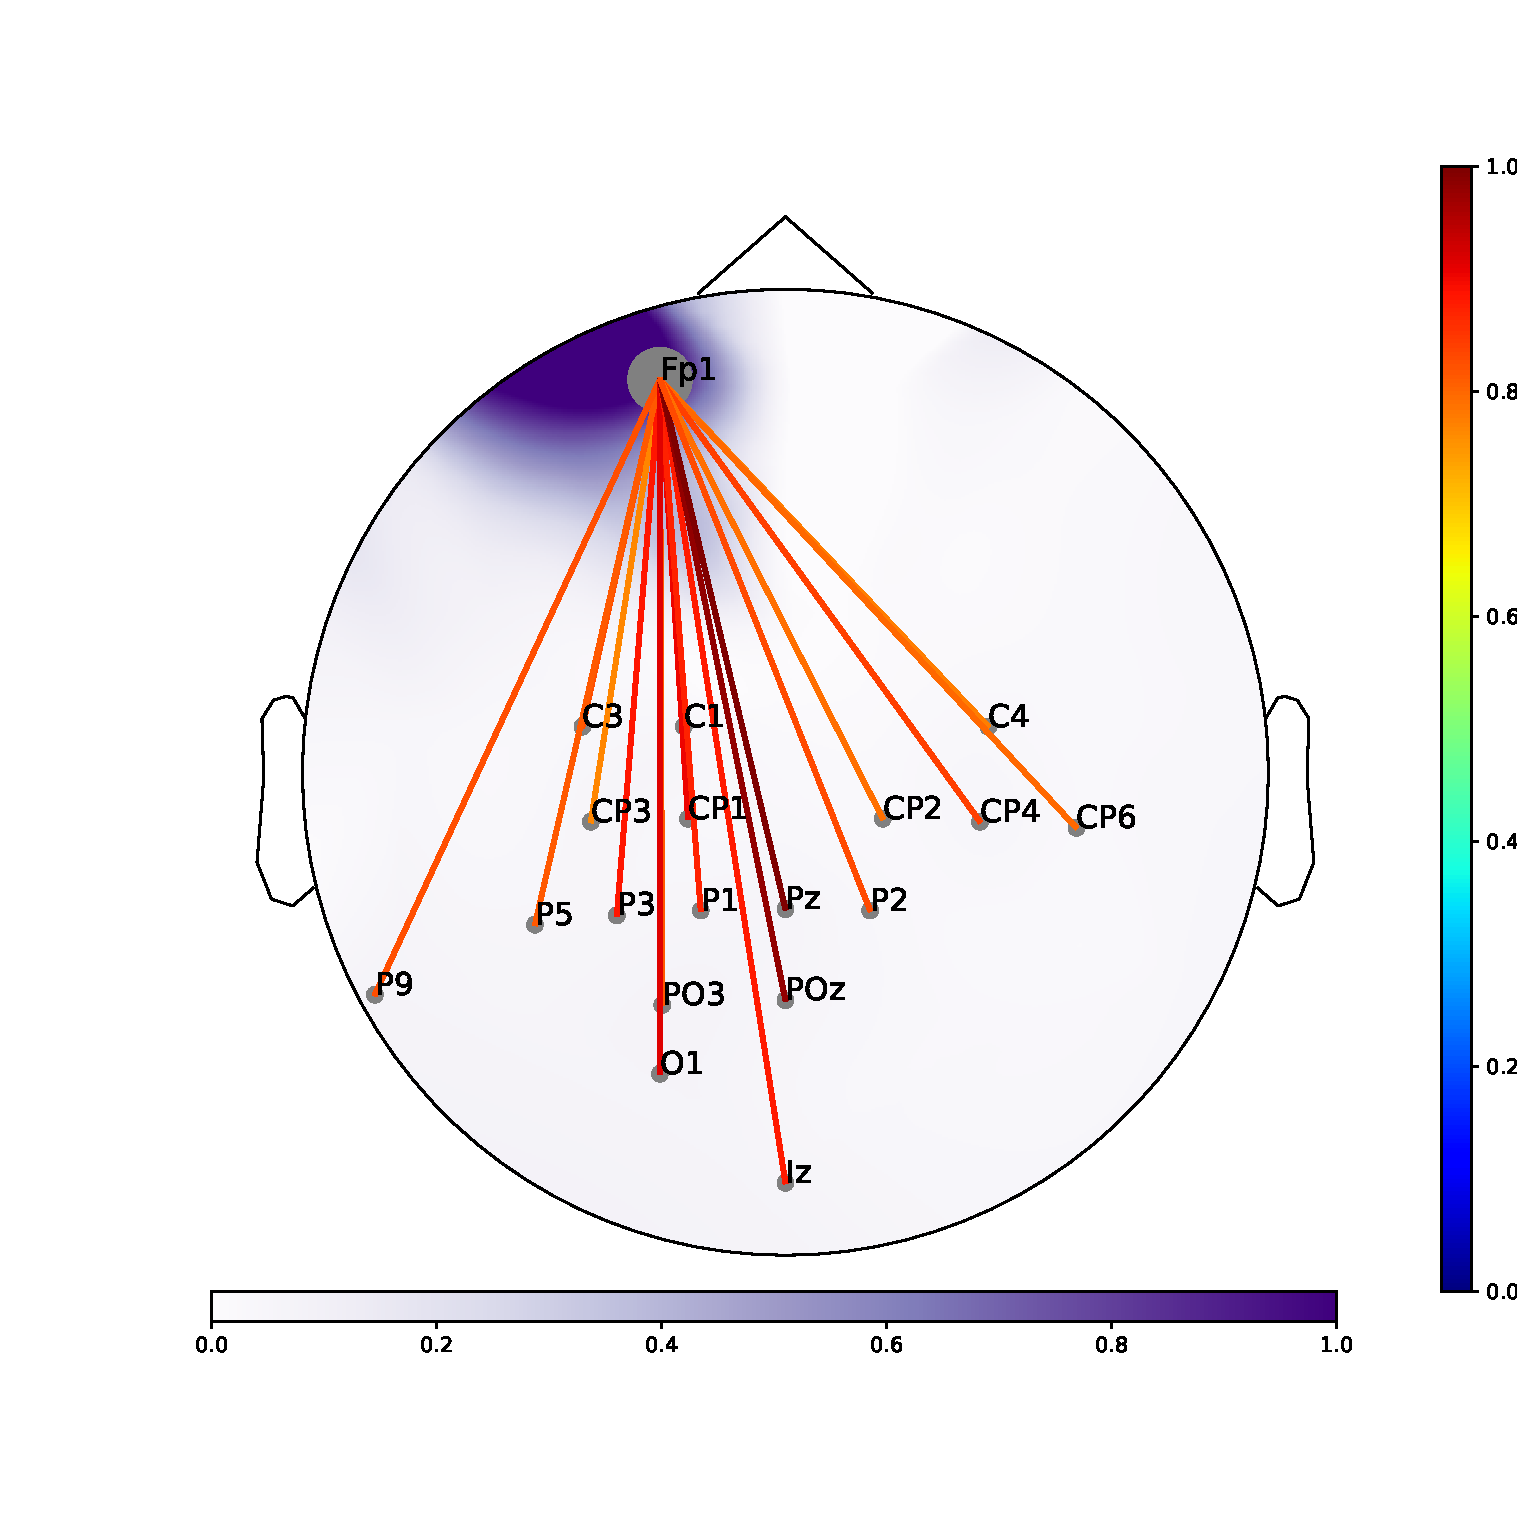
\includegraphics[trim=100 120 90 90, clip]{Figures/Objective_1/Cxsbj2pearsonacc64.62.eps}}}&
	{\resizebox{\kerrwidth}{!}{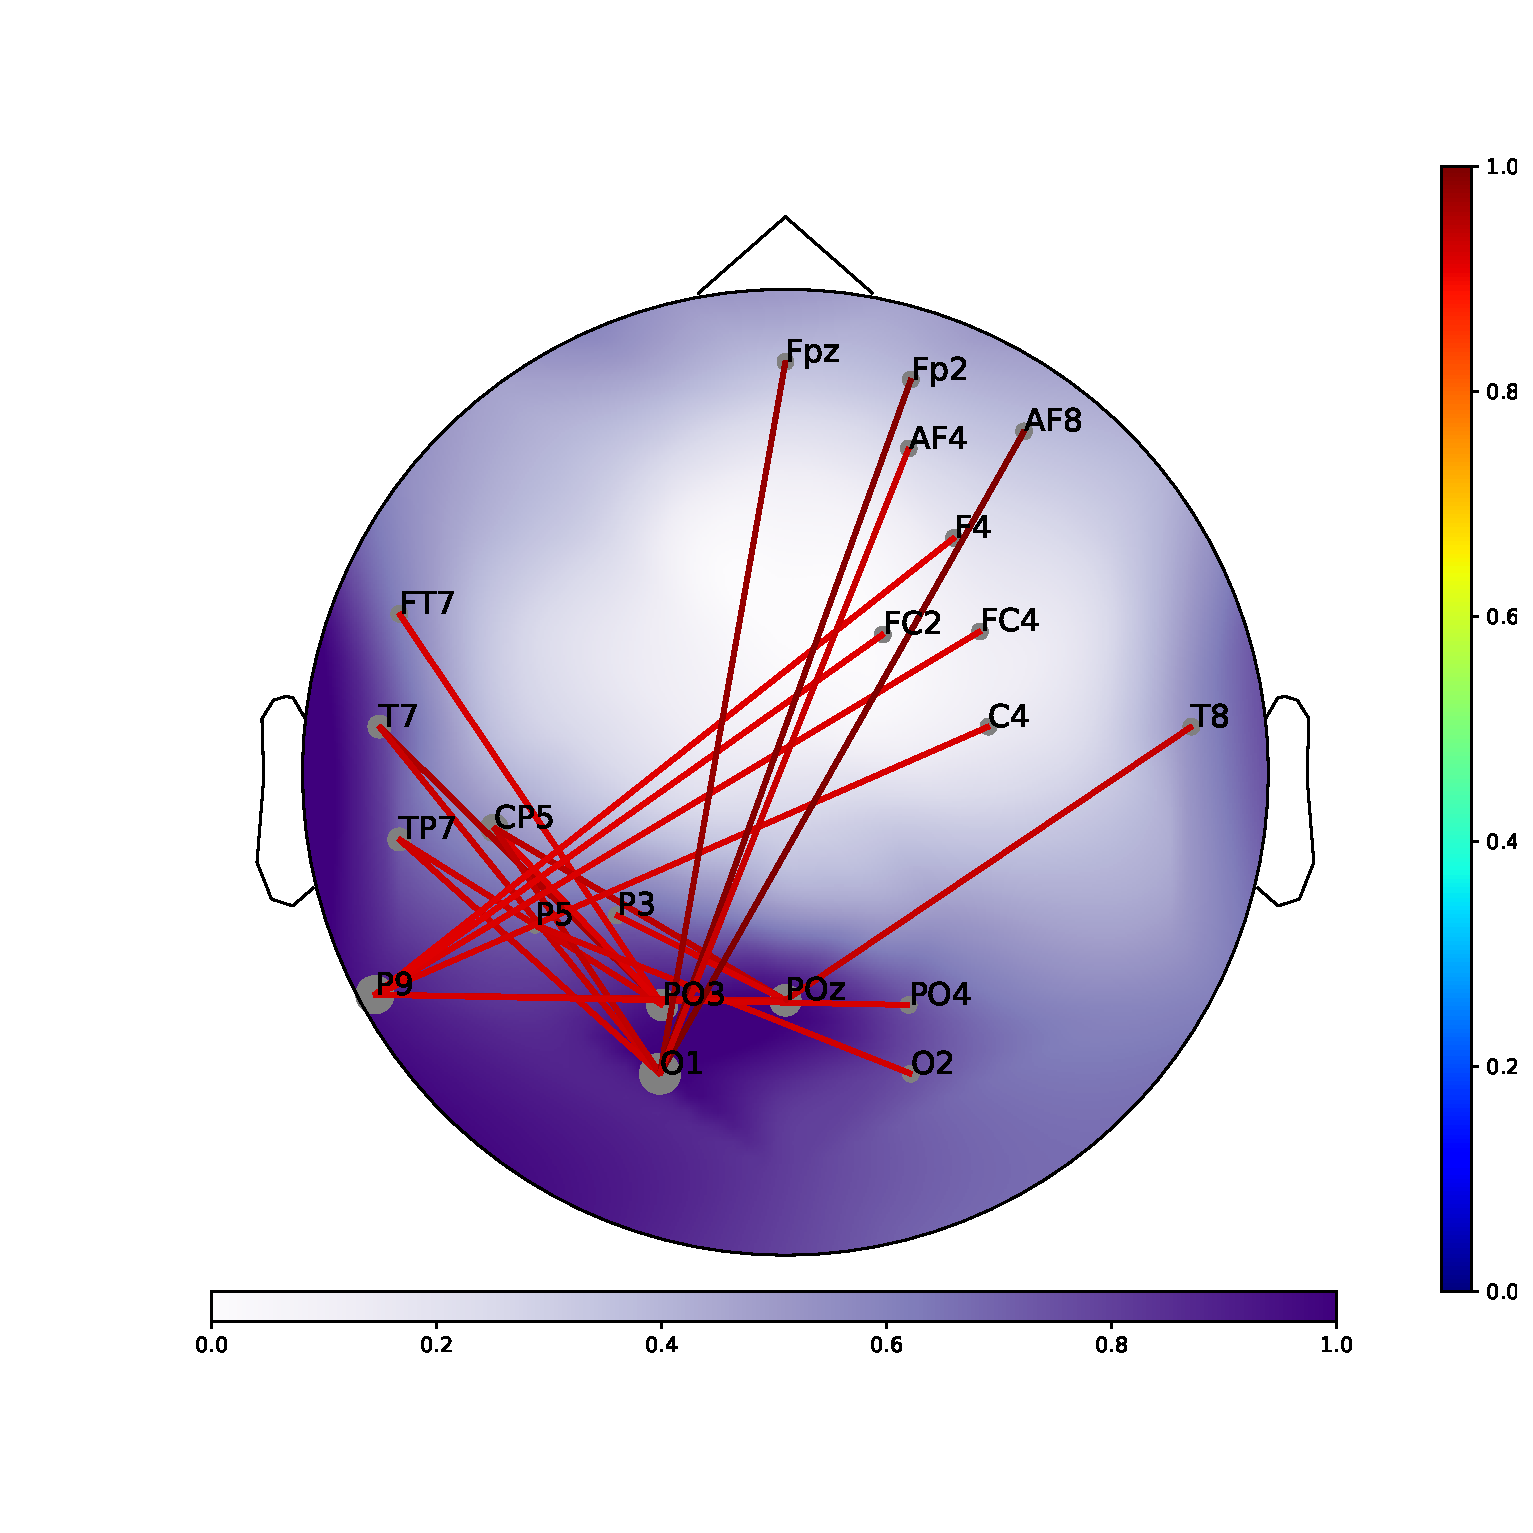
\includegraphics[trim=100 120 90 90, clip]{Figures/Objective_1/Cxsbj3pearsonacc60.69.eps}}}&\\
	& \textbf{$\mathbf{95.28}\%$}& \textbf{$\mathbf{81.16}\%$}& \textbf{$\mathbf{76.09}\%$}& \textbf{$\mathbf{86.85}\%$}& \textbf{$\mathbf{68.93}\%$}& \textbf{$\mathbf{64.4}5\%$}&\\
	\rotatebox{90}{\hspace{7mm} {KCS-FC}}&
	{\resizebox{\kerrwidth}{!}{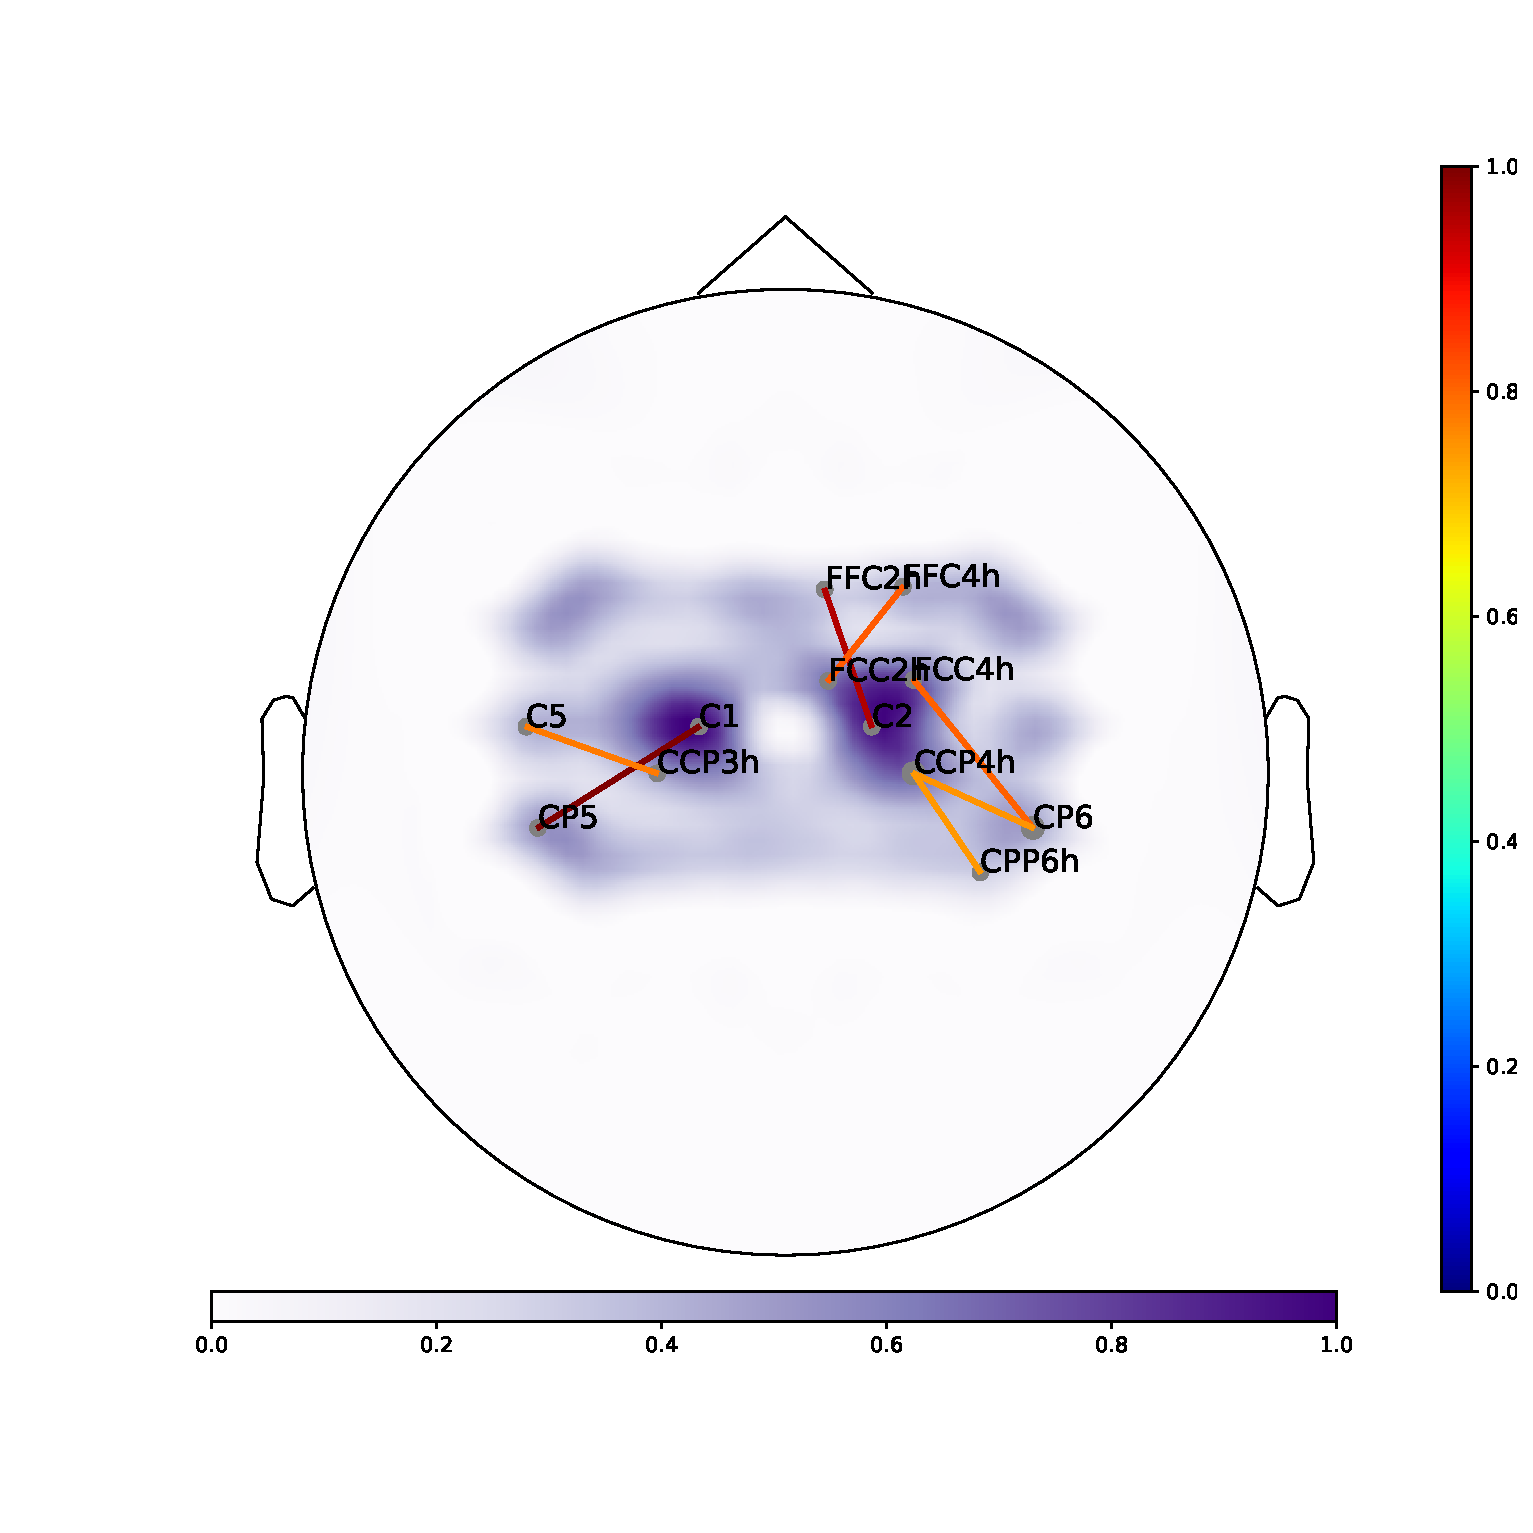
\includegraphics[trim=100 120 90 90, clip]{Figures/Objective_1/Cxsbj1hg-gaussacc95.28.eps}}}&
	{\resizebox{\kerrwidth}{!}{\includegraphics[trim=100 120 90 90, clip]{Figures/Objective_1/Cxsbj2hg-gaussacc81.16.eps}}}&
	{\resizebox{\kerrwidth}{!}{\includegraphics[trim=100 120 90 90, clip]{Figures/Objective_1/Cxsbj3hg-gaussacc76.09.eps}}}&
	{\resizebox{\kerrwidth}{!}{\includegraphics[trim=100 120 90 90, clip]{Figures/Objective_1/Cxsbj1gaussacc86.85.eps}}}&
	{\resizebox{\kerrwidth}{!}{\includegraphics[trim=100 120 90 90, clip]{Figures/Objective_1/Cxsbj2gaussacc68.93.eps}}}&
	{\resizebox{\kerrwidth}{!}{\includegraphics[trim=100 120 90 90, clip]{Figures/Objective_1/Cxsbj3gaussacc64.45.eps}}}&\\
	&\multicolumn{6}{c}{\resizebox{0.85\linewidth}{!}{\includegraphics[trim=0 0 50 600, clip]{Figures/Objective_1/Cxsbj1hg-gaussacc95.28.eps}}}&
\end{tabular}}
\vspace{-42pt}
\caption{Spatial
 relevance mapped to topoplots estimated for each group of individuals from the FC measures (regarding the relevance weights $\ve{v}$ and the classification accuracy). The normalized relevance weights values (between 0 to 1) are computed from Equation~\eqref{eq:SRC}. The background stands for the accumulated spatial relevance mapped to the EEG channel positions. The colored links represent the normalized FC relevance weights that hold a value higher than the $99$ percentile of vector $\ve{v}$. Above each plot, the average accuracy is shown over the corresponding group.}\label{Fig:Topograms}
\end{figure}

In DBIII~ME, the full electrode montage is employed and, thus, the estimated neural responses are all spread over the scalp, as seen in the three last topoplots of every row. Likewise, the number of relevant links increases. Nonetheless, the compared FC measures' performance has some similarities with DBII MI: PLV presents high background activity, CCF has amplitudes with fewer amplitudes, and GCF achieves a very focalized activity over the SMR hemispheres, which play a critical role in MI tasks. Once again, the proposed KCS-FC measure outperforms the values of accuracy attained by other compared FC metrics. However, G III produces highly increased response amplitudes abnormally confined over the frontal zone (outside the SMR zone) and numerous links going to different electrodes. This issue may be explained because of acquisition artifacts, which may introduce noise and distortions, severely damaging the EEG data quality.

\subsection{Selecting the Sliding Time Window} 

The window length selected for extracting the EEG dynamics over time is a pivotal parameter. From the results obtained, both contrasted single-trial FC measures (Cross-Correlation Coefficient and Phase Lag Value) show several fluctuations over the evaluated values of $\tau$ that diminish the performed accuracy, becoming worse in databases with increased subject variability, as is the case of DBIII MI. On the other hand, the proposed Gaussian Functional Connectivity measure enables accuracy estimates that are less affected by the sliding time window and, thus, KCS-FC allows for extracting the subject's dynamics more accurately within wider ranges of $\tau$. 

\subsection{Prior Spatial Filtering Versus to Feed the Concatenation of FC Feature Sets} 

\begin{table}[h!]
	\caption{Classifier accuracy comparison of approaches using functional connectivity features recently reported against the Gaussian FC performance in discriminating MI tasks. Notation TSGSP is temporally constrained sparse group spatial pattern, STR is space-time recurrence, and OPTICAL is Optimized CSP with long short term memory (LSTM). The best value performed for each database is marked in bold.} \label{Tab:Acc}
	\setlength{\tabcolsep}{4.9mm}

\resizebox{\columnwidth}{!}{
\begin{tabular}{cccccc}
	\toprule
		\textbf{Data}& \textbf{Time Window} & \textbf{Filter Band} & \textbf{Interpretation} & \textbf{Feature Extraction}  & \textbf{Accuracy} (\%)\\
		\midrule
		{\multirow{4}{*}{\rotatebox[origin=c]{90}{{DBI-MI}%MDPI: please confirm the text direction. We confirm.
}}} &
		\checkmark&\checkmark&\checkmark&TSGSP~\cite{Zhang2018}&\textbf{82.50} $\pm$ \textbf{12.2}\\
		&-&-&\checkmark&STR connectivity~\cite{rodrigue2019}&69.56$\pm$15.02\\
		& \checkmark & - & \checkmark & Renyi's $\alpha$-entropy~\cite{de2019data} & 72.40 $\pm$ 6.50\\					
		&\checkmark&\checkmark&\checkmark&{Proposed KCS-FC}& {81.92} $\pm$ {9.44}\\
		\midrule	
		{\multirow{4}{*}{\rotatebox[origin=c]{90}{DBIII-MI}}} &		
		- &\checkmark&\checkmark & CSP~\cite{cho2017eeg}&67.60 $\pm$ 13.17\\
		&\checkmark&\checkmark&-&OPTICAL~\cite{kumar2019brain}&68.19 $\pm$ 9.36\\
		&-&-&\checkmark&STR connectivity~\cite{rodrigue2019}&62.00 $\pm$ 13.00\\	
		&\checkmark&\checkmark&\checkmark&{Proposed KCS-FC}&\textbf{74.12} $\pm$ \textbf{12.13} \\\bottomrule
	\end{tabular}
 }
\end{table}

Because of the poor signal-to-noise ratio of scalp EEG measurements, the baseline CSP-based spatial filtering is very frequently accomplished. Meanwhile, the evaluating results indicate that the CSP effectiveness degrades noticeably as the inter/intrasubject variability increases. Thus, a big partition of subjects in DBIII MI turns out to be below the BCI-inefficiency level. These findings are according to the reported CSP variability from trial-to-trial~\cite{Gaur2021}, and the subject-dependent choice of its extraction window~\cite{Velasquez-Martinez2020}. 

One more restriction is that CSP is more oriented to power-based features~\cite{kumar2018eeg}, so that its validity of the combination with PLV is questionable, as the achieved results definitely indicate. The combination of CSP with CCF and KCS-FC allows for enhancing the performed accuracy, but in DBI~MI and DBII~ME with a relatively moderate number of subjects. The testing of DBIII~MI with the largest considered intra/inter-subject variability tends to nullify CSP filtering before CCF feature extraction. Moreover, the proposed KCS-FC measures' performance improves if avoiding using the spatial filtering algorithm, which means that FC feature sets' straightforward concatenation is enough to feed the sparse-based $\ell_2$-norm feature selection framework. Table \ref{Tab:Acc} displays the evaluated MI data's accuracy (i.e.,~DBI MI, and DBIII MI) using functional connectivity measures that have been reported recently, noting that the proposed KCS-FC approach provides very competitive classifier performance values.



\section{Summary}

We have introduced a novel method for single-trial kernel cross-spectral functional connectivity, known as KCS-FC, which addresses prevalent challenges inherent to EEG-based MI-BCI systems, identified in \cref{sec:singlefc}. These include issues related to non-stationarity, non-linearity, inter-subject variability, and spurious connectivities. To achieve this, we applied an extension of Bochner's theorem to approximate the cross-spectral distribution as a weighted sum of Gaussian-kernel-based pairwise relationships between channels, considering various time windows and frequency sub-bands. This weighted sum is managed by a linear regression model combined with an elastic net regularization that aligneds the value with the MI label and differentiates spurious connectivities. In testing our method, we compared it with two prevalent single-trial FC estimators and respective CSP versions using two publicly available MI datasets. The results reveal that our KCS-FC strategy shows competitive accuracy in performance while maintaining interpretable FC matrices.

However, our approach heavily relies on handcrafted feature extraction processes, including time windowing and sub-band selection. This reliance on handcrafted features, as discussed in \cref{sec:problem2}, does not significantly assist in artifact removal and only marginally increases accuracy for lower-performing individuals. Future research, as suggested in \cref{sec:sota2}, should focus on adopting end-to-end DL models that can autonomously extract EEG representations. This would potentially be more effective in removing artifacts and could potentially enhance the performance of low-performing individuals.
